\section{Implementación}\label{implementacionPosta}
Un sistema de captura de movimiento con las características necesarias para cumplir el objetivo de este proyecto debe implementar cuatro bloques generales: \emph{calibración}, \emph{detección de marcadores}, \emph{reconstrucción} y \emph{seguimiento}. En la Figura \ref{bloquesSist} se muestra un esquema del sistema a implementar, cada bloque verde indica la salida de una etapa siendo  a su vez la entrada del bloque siguiente.
%\vspace{-0.6cm}
\begin{figure}[ht!]
	\centering
	\hspace{-0.5cm}
	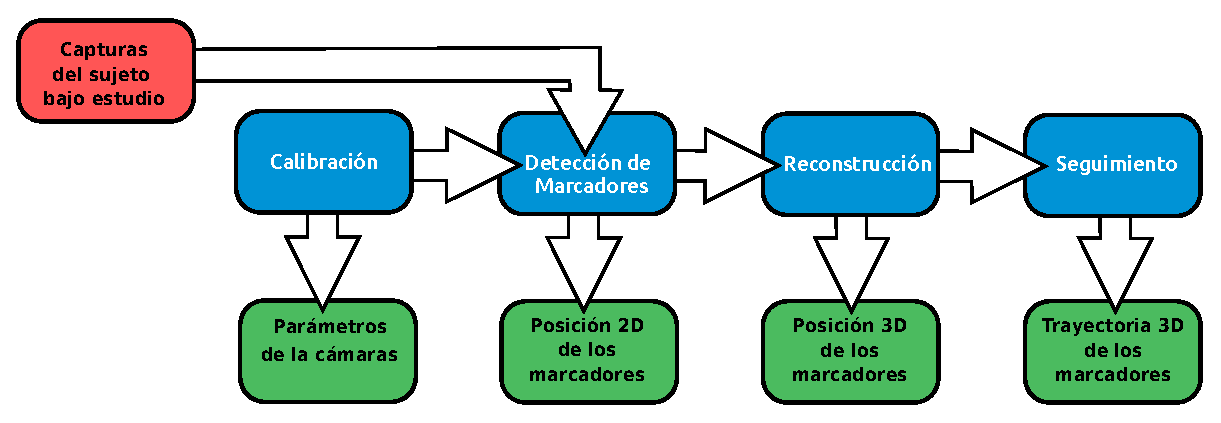
\includegraphics[scale=0.55]{imagenes/Sistema_completo/Diagrama_de_bloques.eps}
	\caption{Diagrama de bloques del sistema completo.}
	\label{bloquesSist}
\end{figure}
%\vspace{-0.7cm}
%Es importante destacar el hecho de poder separar el sistema en bloques independientes,

Es importante destacar la independencia entre bloques, permitiendo modificar u optimizar fácilmente el sistema en etapas futuras.
A continuación se describe el funcionamiento de cada etapa del proceso de captura de movimiento, asi como su implementación.
\chapter{Calibración}\label{calibracion}


\section{Introducción}
Para poder obtener la posición en tres dimensiones de los marcadores a partir de las imágenes capturadas es necesario que las cámaras estén previamente calibradas. El objetivo de la calibración consiste en determinar un conjunto de parámetros tal que pueda establecerse una relación entre el espacio 3D y las coordenadas 2D de las imágenes.\\
\vspace{-0.1cm}


Los puntos en el espacio pueden ubicarse respecto a un sistema de coordenadas 3D. A su vez, los puntos capturados en las imágenes pueden referenciarse respecto a un sistema de coordenadas 2D en píxeles. Si se quiere determinar la posición de un punto en el espacio en función de las correspondientes proyecciones de dicho punto en las imágenes capturadas por las cámaras, es necesario determinar las ecuaciones que vinculan al sistema de coordenadas del espacio con el sistema de coordenadas en píxeles de las cámaras.\\

De la relación entre estos sistemas de coordenadas se obtienen los parámetros de las cámaras. Dichos parámetros se clasifican en intrínsecos y extrínsecos. Los primeros son aquellos que describen las propiedades geométricas y ópticas de la cámara, es decir, las características internas de la cámara. Por otra parte, los parámetros extrínsecos son los que describen la posición y orientación de la cámara respecto al sistema de coordenadas del espacio.\\

Para realizar esto es necesario establecer un modelo que describa el sistema óptico de las cámaras. Esto es, el modelo por el cual una cámara es capaz de transformar el espacio 3D en imágenes de dos dimensiones. Un modelo simple y que describe estos sistemas adecuadamente es el modelo \textit{pinhole} de las cámaras. 
El modelo \textit{pinhole} se basa en la implementación mas simple de una cámara real, la cámara estenopeica. En dicha cámara la imagen capturada esta conformada por la proyección del espacio 3D a través de un punto situado delante de la retina de la cámara como se muestra en la figura \ref{pinhole_camara}. El modelo de esta cámara se describe en la figura \ref{pinhole_modelo}.\\

\begin{figure}[ht!]
\begin{center}
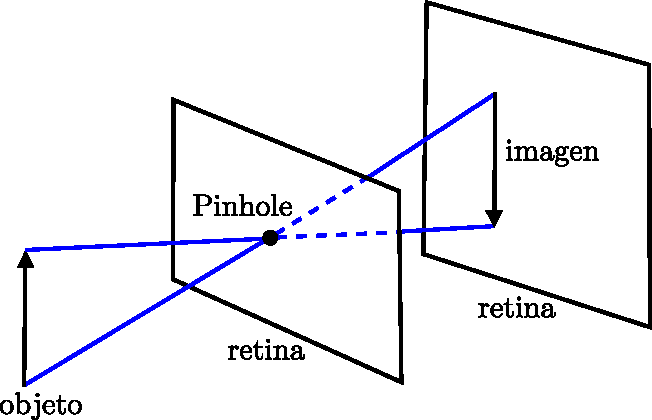
\includegraphics[scale=0.5]{img/calibracion/pinhole_camara}
\end{center}
\caption{Cámara estenopeica .\cite{faugeras_libro}}
\label{pinhole_camara}
\end{figure}



\begin{figure}[ht!]
\begin{center}
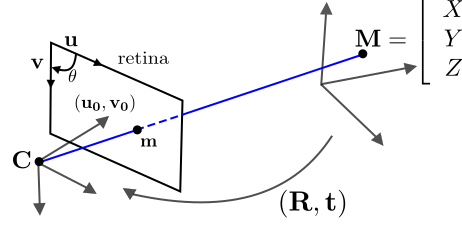
\includegraphics[scale=0.5]{img/calibracion/pinhole_modelo}
\end{center}
\caption{Modelo "pinhole" de una cámara.\cite{zhang_libro}}
\label{pinhole_modelo}
\end{figure}

En dicho modelo, una cámara se representa por un punto $C$, foco de la cámara, y un plano, al  que se le llama retina de la cámara. La imagen que se proyecta en la retina corresponde a la imagen capturada por la cámara. Dado un punto $M$ en el espacio, su correspondiente proyección en la retina, el punto $m$, se encuentra en la intersección de la retina y la recta formada por los puntos $C$ y $M$ de manera que $C$, $M$ y $m$ son colineales.\\ 




Si las coordenadas del punto  $M$ y las del punto $m$ son las siguientes:


\[m = \begin{bmatrix}
u \\ 
v
\end{bmatrix} , \quad
M = \begin{bmatrix}
X \\ 
Y \\
Z
\end{bmatrix} \]

Notando con $\tilde{x}$ a los vectores en coordenadas homogéneas se tiene:

% ANEXO EXPLICANDO COORDENADAS HOMOGÉNEAS??

\[\tilde{m} = \begin{bmatrix}
u \\ 
v \\
1
\end{bmatrix} , \quad
\tilde{M} = \begin{bmatrix}
X \\ 
Y \\
Z \\
1
\end{bmatrix} \]

Tomando el modelo \textit{pinhole} de la cámara, la relación entre un punto $M$ y su proyección $m$ es:
\begin{equation}
s\tilde{m} = A [R \quad t]\tilde{M}
\label{proyeccion}
\end{equation}




\begin{equation}
\text{siendo }
A = \begin{bmatrix}
\alpha & c & u_0 \\ 
0 & \beta & v_0 \\ 
0 & 0 & 1
\end{bmatrix} 
\end{equation}

Por lo tanto estos puntos se relacionan a través de la matriz $P = A [R \quad t]$, a menos de un factor de escala $s$. A dicha matriz  se le denomina Matriz de Proyección de la cámara.\\

La matriz $P$ se compone a su vez de la matriz $A$ que representa los parámetros intrínsecos de la cámara, y la matriz $[R \quad t]$ que representa los parámetros extrínsecos.\\

La matriz $[R \quad t]$ está formada por la rotación y traslación que relaciona el sistema de coordenadas del espacio con el sistema de coordenadas de la cámara. La matriz $A$ está formada por los parámetros intrínsecos de la cámara:\\



\begin{tabular}{cp{.8\textwidth}}


$(u_0, v_0)$ &  coordenadas del punto principal. \\ 
$\alpha$ y $\beta$ & factores de escala en los ejes de imagen  $u$ y $v$. \\ 
$c$ & grado de oblicuidad de los ejes imagen
\end{tabular} \\

El punto principal $(u_0, v_0)$ se define como el punto formado por la intersección de la retina y la recta perpendicular a dicha retina que pasa por el punto $C$. La distancia entre el punto $C$ y el punto principal se define como la distancia focal de la cámara $f$. Los factores $\alpha$ y $\beta$ se relacionan con la relación de aspecto de los píxeles de la cámara. El parámetro $c$ se relaciona con el ángulo $\theta$ formado por los ejes $u$ y $v$.\\

Por lo tanto la proyección de un punto 3D sobre la retina se compone de los siguientes pasos:\\

\begin{itemize}
\item Se pasa del sistema de coordenadas del espacio 3D $(X_w, Y_w, Z_w)$ al sistema de coordenadas de la cámara $(X,Y, Z)$
\begin{equation}
[X \ Y \ Z] = [X_w \ Y_w \ Z_w]^T + t
\end{equation}
\item Se proyecta el punto 3D respecto a las coordenadas de la cámara sobre las coordenadas imagen de la retina $(x,y)$.
\begin{equation}
x=f \dfrac{X}{Z} \qquad y = \dfrac{Y}{Z}
\end{equation}
\item En algunos casos puede ser necesario modelar además ciertas distorsiones introducidas por el lente de la cámara.
\begin{equation}
\check{x} = x + \delta_x \qquad \check{y} = y + \delta_y
\end{equation}

Siendo $(\check{x},\check{y})$ las coordenadas distorsionadas y $(\delta_x, \delta_y)$ las distorsiones aplicadas a $(x,y)$.

\item Por último se pasa de la coordenadas imagen $(\check{x}, \check{y})$ a las coordenadas en píxeles $(\check{u}, \check{v})$.
\vspace{-0.05cm}
\begin{equation}
\check{u} + d_x ^{-1}\check{x} + u_0 \qquad \check{v} + d_y ^{-1}\check{y} + v_0
\end{equation}

Siendo $d_x$ y $d_y$ las distancias entre píxeles adyacentes en las direcciones horizontal y vertical, respectivamente.\\
\end{itemize}


\section{Métodos de calibración}

De acuerdo a los objetos utilizados para realizar la calibración, los métodos pueden clasificarse de la siguiente manera \cite{zhang_libro}:\\

\begin{itemize}
\item Calibración mediante objetos 3D\\

La calibración mediante este método es realizada capturando la imagen de un objeto de calibración cuyas dimensiones y geometría son conocidas. Los objetos de calibración suelen ser planos colocados ortogonalmente. También pueden utilizarse estructuras con marcadores de dimensiones conocidas. A estos objetos se les aplica traslaciones en el espacio logrando más cantidad de puntos de referencia para calibrar. La ventaja de este método es su precisión aunque se requiere de objetos más costosos y procedimientos más elaborados.\\

\item Calibración mediante objetos 2D\\

Este caso se utiliza objetos planos con figuras de patrones determinados, por ejemplo dameros. Estos objetos son colocados en varias posiciones delante de la cámara de manera de capturar varias imágenes del objeto. Esta metodología ofrece más flexibilidad para calibrar.\\

\item Auto calibración\\

Este método consiste en obtener la información necesaria a través de la captura de varias imágenes de un escena estática, prescindiendo de objetos para calibrar. Esta método es más flexible que  los anteriores aunque suele ser menos preciso.\\

\end{itemize}


Algunas soluciones comerciales, como por ejemplo Vicon \footnote{\textcolor{blue}{\underline{\url{http://www.vicon.com}}}. Accedido 3-12-14.} , utiliza como objeto de calibración una vara con leds, ver figura \ref{vicon}. 

\begin{figure}[ht!]
        \centering
        
        \subfloat{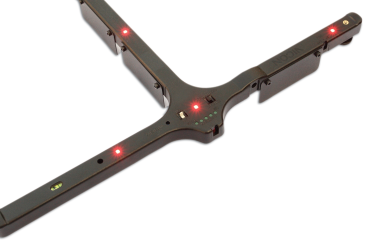
\includegraphics[scale=1.8]{img/calibracion/vicon1.png}}
        \hspace{1.8cm}
        \subfloat{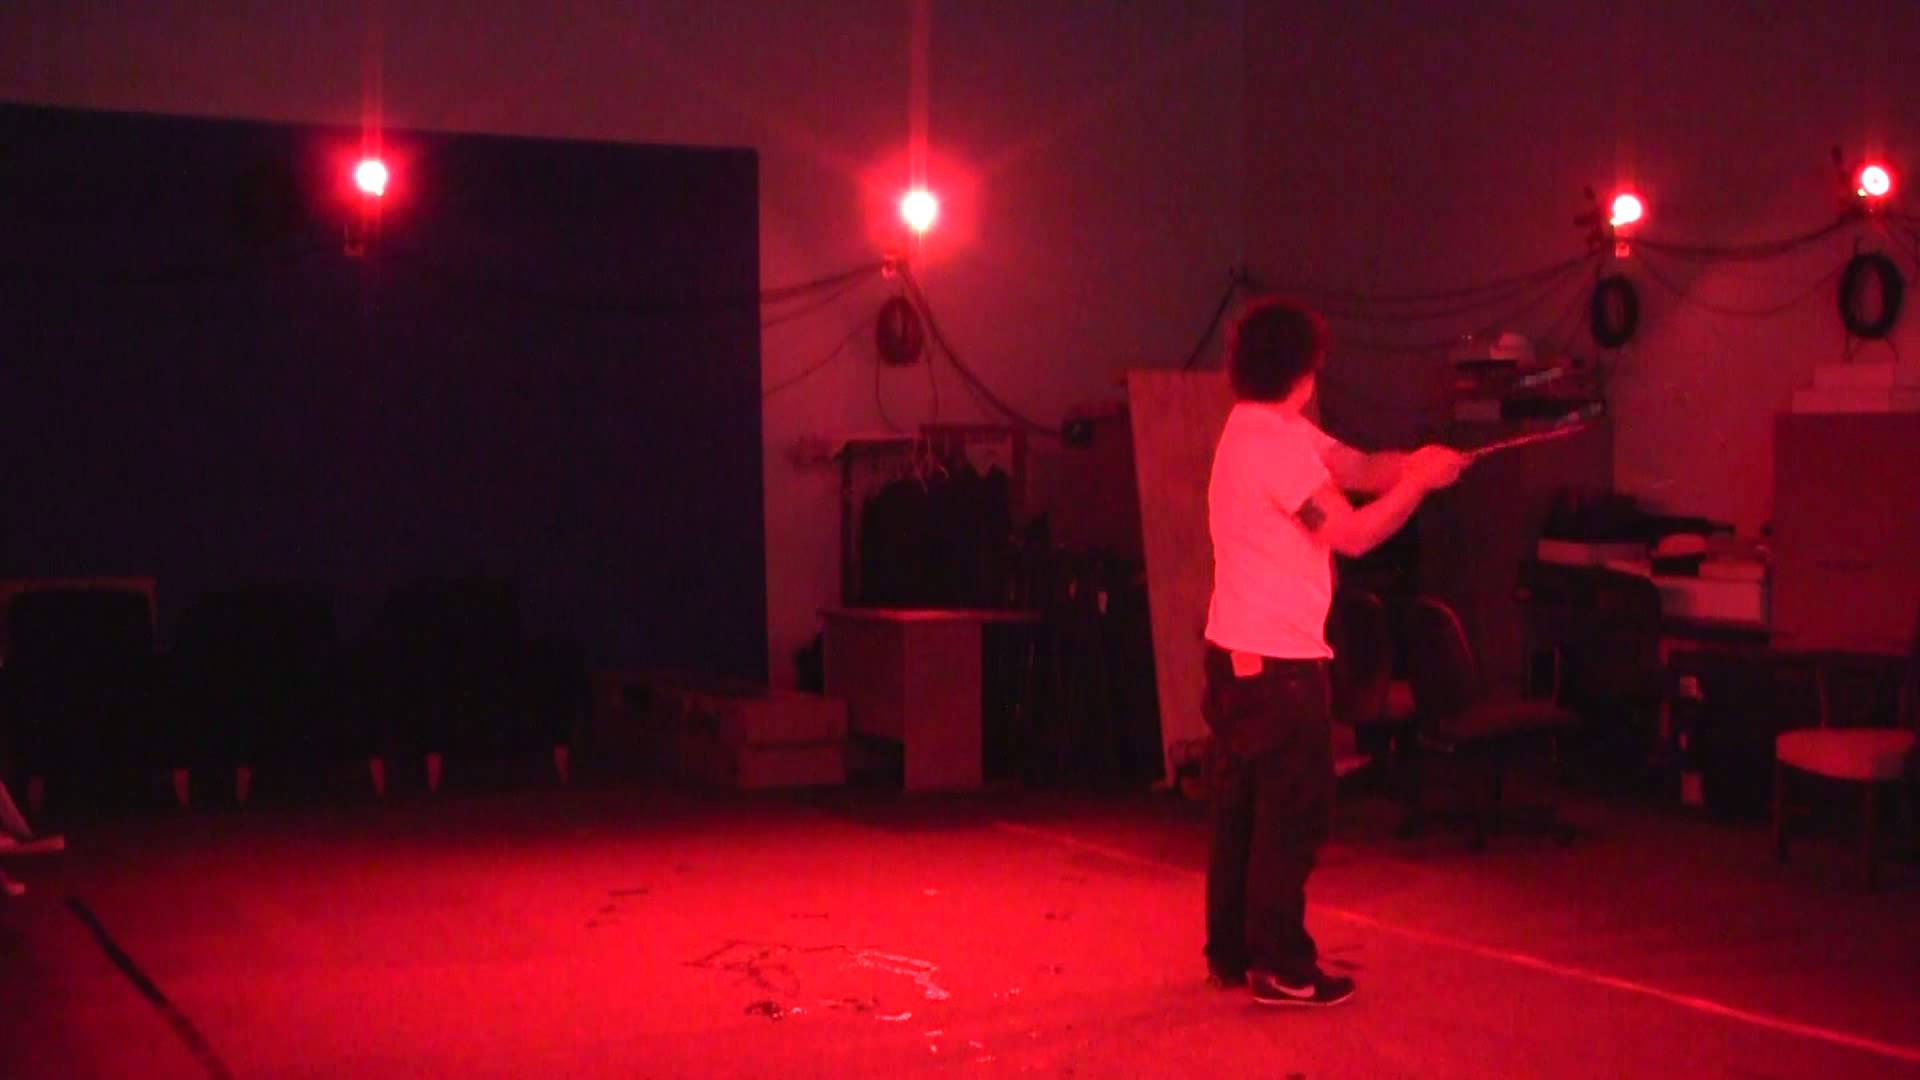
\includegraphics[scale=0.08]{img/calibracion/vicon2.jpg}}
  \caption{Calibración Vicon}
      \label{vicon}
\end{figure}

En este caso la calibración se realiza moviendo el objeto de calibración a través del espacio de trabajo. Este método resulta muy flexible para la calibración de un conjunto de varias cámaras simultáneamente.


\section{Calibración en el entorno Blender}

Una vez establecida la configuración de las cámaras en  Blender, según lo descrito en la sección \ref{section_base_de_datos}, es posible conocer las matrices de proyección de cada una de ellas a través de la información proporcionada por el propio programa de ciertos parámetros de las cámaras. Esto permite tener la calibración \textit{real} de las cámaras con lo cual es posible medir el desempeño de algunos bloques del sistema.\\

Si se conocen las coordenadas de un punto 3D en el espacio de trabajo de Blender y además se saben las matrices de proyección de las cámaras, es posible determinar las coordenadas 2D de dicho punto proyectado en cada una de las cámaras. De esta manera se tiene el \textit{ground truth} de la detección de marcadores, permitiendo comparar el desempeño de dicho bloque respecto  a la posición real de los marcadores en las vistas 2D. Análogamente teniendo estos datos se pueden evaluar los bloques siguientes del sistema. Por ejemplo, es posible además evaluar el desempeño del bloque de reconstrucción sabiendo la posición 2D real de los marcadores, por lo cual se puede evaluar los errores que son producto solamente de este bloque del sistema.\\

A continuación se describe cómo se deducen las matrices de proyección a partir de ciertos parámetros proporcionados por el programa.\\

La posición de una cámara se establece respecto a un sistema de coordenadas determinado, al que se le puede llamar el sistema de coordenadas del mundo. Por lo cual es posible saber la rotación y traslación que es necesario aplicar al sistema de coordenadas del mundo para obtener el sistema de coordenadas solidario a la cámara. Los parámetros que se pueden obtener de Blender son los ángulos de rotación $(\theta, \phi, \psi )$ respecto a los ejes $(x,y, z)$ del sistema de coordenadas del mundo, así como el orden en que se ejecutan dichas rotaciones. Si el orden establecido es \textit{XYZ Euler}, lo que implica que primero se rota respecto al eje $x$, luego al $y$ y al $z$, se obtiene la matriz de rotación:

\[R=R_{(z,\psi)}R_{(y,\phi)}R_{(x,\theta)}
= \begin{pmatrix}
		r_{11} & r_{12} & r_{13}\\
		r_{21} & r_{22} & r_{23}\\
		r_{31} & r_{32} & r_{33}\\ 
\end{pmatrix}= 
\begin{pmatrix}
			R_1 \\
			R_2 \\
			R_3 \\
		\end{pmatrix}
\]
 
 Donde,
 \[R_{(x,\theta)} = \begin{pmatrix}
		1 &   0         &  0\\
		0 & cos\,\theta & -sen\,\theta\\
		0 & sen\,\theta & cos\,\theta\\ 
\end{pmatrix}, ~
R_{(y,\phi)}=\begin{pmatrix}
		cos\,\phi  & 0 & sen\,\phi\\
		0          & 1 & 0\\
		-sen\,\phi &0  & cos\,\phi\\ 
\end{pmatrix}, ~
R_{(z,\psi)}\begin{pmatrix}
		cos\,\psi & -sen\,\psi & 0\\
		sen\,\psi & cos\,\psi  & 0\\
		 0          & 0            & 1\\ 
\end{pmatrix}\]

A su vez también es posible obtener el vector de traslación $T$ que es necesario aplicar al sistema de coordenadas del mundo para obtener el sistema solidario a la cámara. De esta manera se obtiene la matriz de parámetros extrínsecos:
\[
		M_{ext}=\begin{pmatrix}
			r_{11} & r_{12} & r_{13} &-R^t_1 T\\
			r_{21} & r_{22} & r_{23} &-R^t_2 T\\
			r_{31} & r_{32} & r_{33} &-R^t_3 T\\
		\end{pmatrix}
\] 

Para hallar la matriz de parámetros intrínsecos se necesitan saber los siguientes parámetros que son proporcionados por Blender: 
\begin{itemize}
\item $f$, distancia focal
\item $(o_x, o_y)$, coordenadas del punto principal
\item $(s_x,s_y)$, tamaño efectivo de los píxeles de la retina en píxeles/milímetro.
\end{itemize}

con estos parámetros se obtiene la matriz de parámetros intrínsecos:

\[M_{int}=\begin{pmatrix}
			-f/s_x & 0      & o_x\\
			0      & -f/s_y & o_y\\
			0      & 0      & 1\\
		\end{pmatrix} \]
 
%%%%%%%%APÉNDICE%%%%%%%%%%%%%%%%%%%55
%En el apéndice \ref{apendice_calibracion_blender} se describe en detalle cómo se obtienen los parámetros necesarios en Blender.\\

\section{Calibración para secuencias reales}

\label{seccion_calibracion_secuencias_reales}

%%%%%%%%%%%%REFERENCIAS%%%%%%%%%%%%%%%%%
% LIC DARIO SANTOS, HOSPITAL DE CLÍNICAS

Por intermedio del Lic. Darío Santos, hemos podido tener acceso a secuencias de vídeo de análisis del movimiento de la marcha que se han realizado en el Hospital de Clínicas. Dichas secuencias han sido obtenidas por un grupo de médicos e investigadores con el objetivo de analizar el movimiento de pacientes, es decir, con fines terapéuticos o con un objetivo esencialmente de investigación, en particular del estudio de la marcha humana desde el punto de vista de la biomecánica.\\

%DEBERÍA ACLARARSE QUE ESTO SE HACIA ANTES, CREO QUE TIPO POR 2009 Y AHORA USAN VICON.

La metodología utilizada consiste en el uso de tres cámaras de vídeo convencionales de 25 fps y resolución  720 x 576 píxeles. Dichas cámaras se disponen como se muestra en la figura \ref{fig: lab_real}, alrededor de una alfombra o cinta sobre la que se le pide al paciente que camine.


\begin{figure}[ht!]
\centering
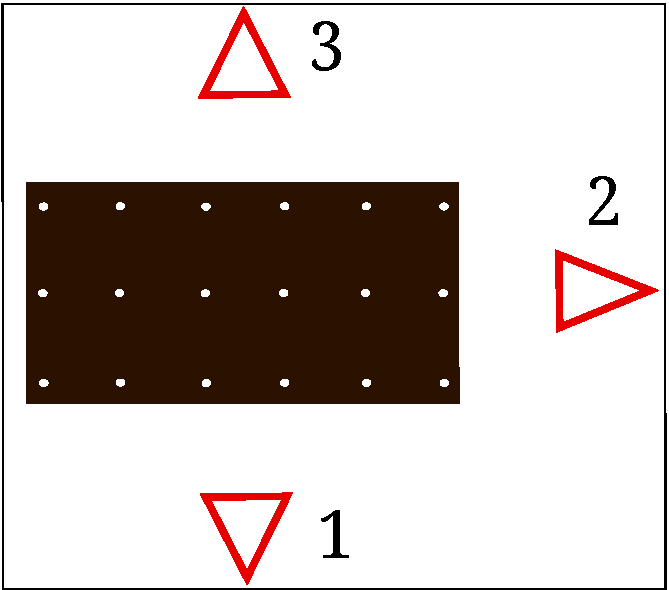
\includegraphics[scale=0.5]{img/calibracion/lab_real.pdf}
\vspace{-0.3cm}
\caption{Laboratorio del Hospital de Clínicas}
\label{fig: lab_real}
\end{figure}

La persona que se desea evaluar debe tener colocados marcadores, fundamentalmente en las articulaciones del cuerpo, y debe desplazarse sobre la alfombra dispuesta para esto. En la figura \ref{fig: persona con marcadores}, se observa a un individuo caminando con los marcadores colocados.

\begin{figure}[ht!]		
        \subfloat[Persona con marcadores]{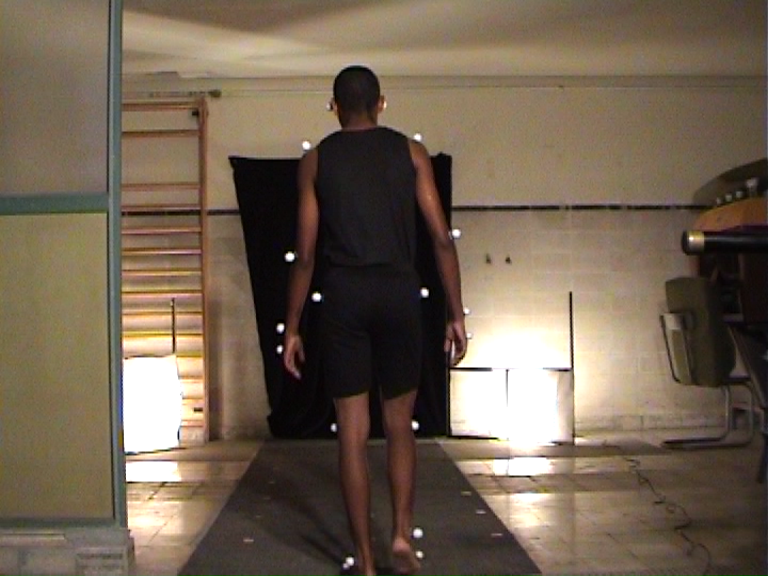
\includegraphics[scale=0.28]{img/calibracion/captura_real.png}\label{fig: persona con marcadores}}
        \hspace{0.1cm}
        \subfloat[Objeto de calibración]{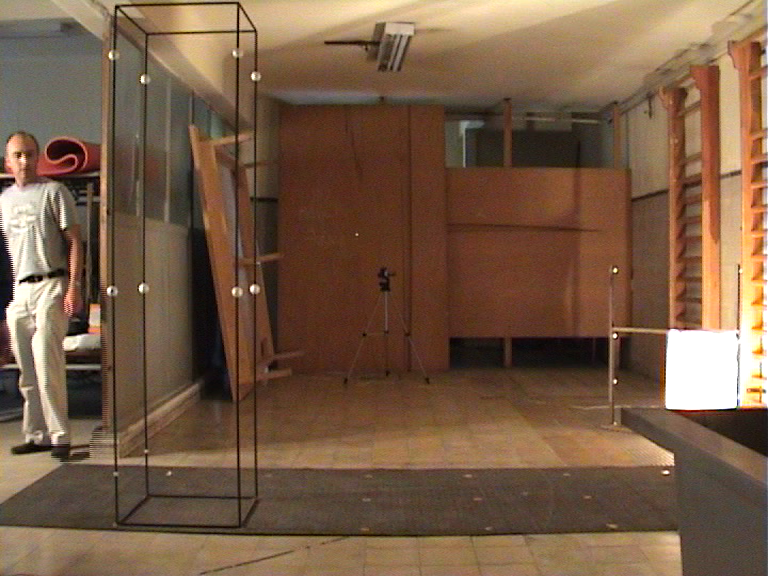
\includegraphics[trim = 20mm 0mm 40mm 0mm, clip, scale=0.28]{img/calibracion/calibrador.png}\label{fig: calibrador}}
  \caption{Captura de secuencia real}
      \label{fig: captura real}
\end{figure}

Antes de la captura del movimiento se emite una señal acústica con la cual se sincronizan las tres vistas una vez obtenidos los vídeos. El software con el cual este grupo de médicos han analizado el movimiento es el \textit{Dvideow}.            
 %%%%%%%%%%%%%%%%%%(REFERENCIAR)%%%%%%%%%%%%%%%%%%%%%%%%%%%%%%. 
 Dicho software realiza la detección, seguimiento y reconstrucción de los marcadores. No hemos podido tener acceso a este software por lo cual tampoco pudimos evaluar su desempeño y compararlo con el desarrollado por nosotros.\\

Para calibrar este sistema se utiliza el objeto de calibración, o calibrador, como se muestra en la figura \ref{fig: calibrador} que consiste en marcadores colocados sobre una estructura de dimensiones conocidas. Dicho objeto se coloca sobre distintos puntos marcados sobre la alfombra, por lo que las traslaciones realizadas son de distancias conocidas. De esta manera se calibra con más puntos sobre el volumen de trabajo.\\


El método implementado requiere que cada marcador del calibrador, en cada una de las vistas, sea seleccionado manualmente en un orden tal que permita establecerse una correspondencia entre las proyecciones de un mismo marcador en las tres vistas. En la figura \ref{fig: vistas_calibrador} se muestra a uno de los marcadores seleccionado en cada una de las vistas.\\


\begin{figure}[ht!]
        \hspace{-1cm}
        \subfloat[Vista cámara 1]{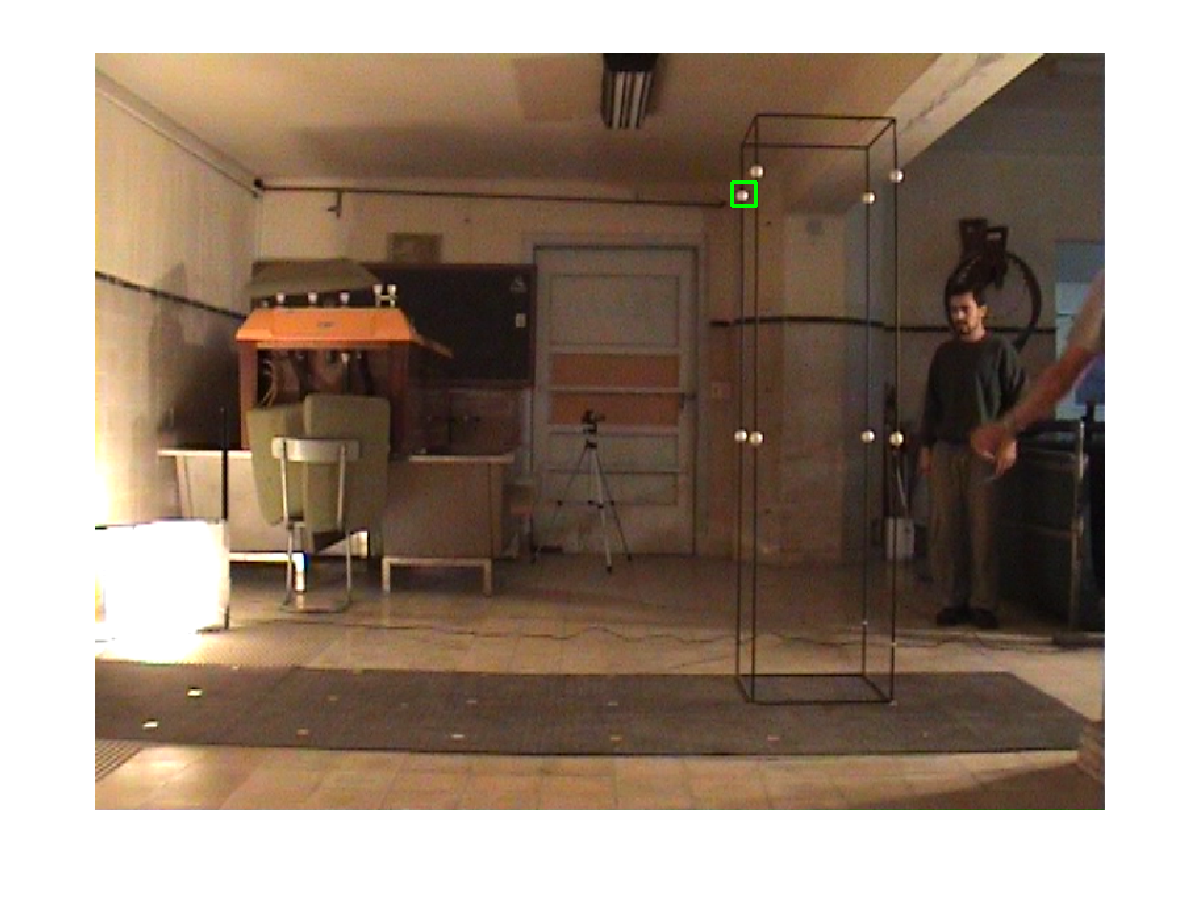
\includegraphics[trim = 59mm 0mm 41mm 0mm, clip,scale=0.45]{img/calibracion/calibrador_cam1.png}}
                \hspace{1mm}
        \subfloat[Vista cámara 2]{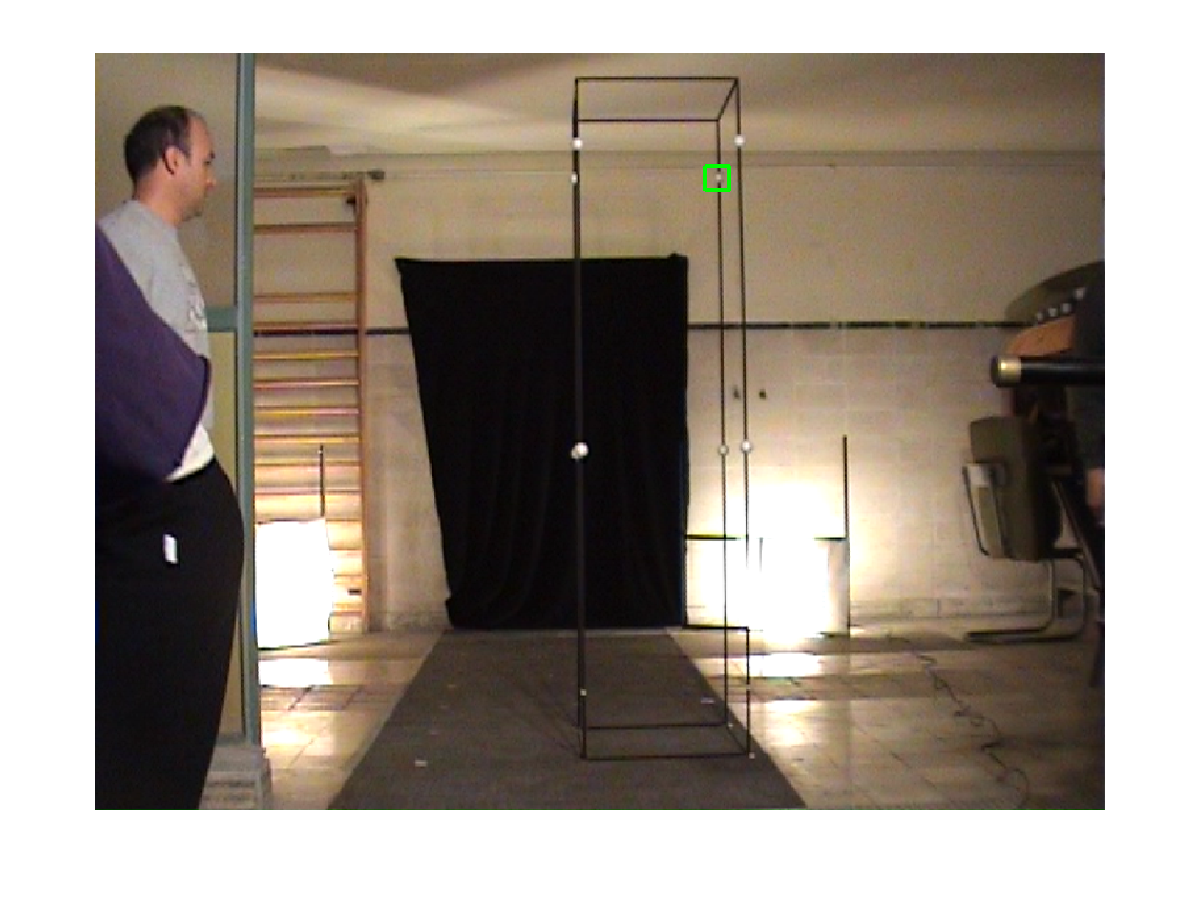
\includegraphics[trim = 50mm 0mm 50mm 0mm, clip,scale=0.45]{img/calibracion/calibrador_cam2.png}}     	
  \hspace{1mm}
        \subfloat[Vista cámara 3]{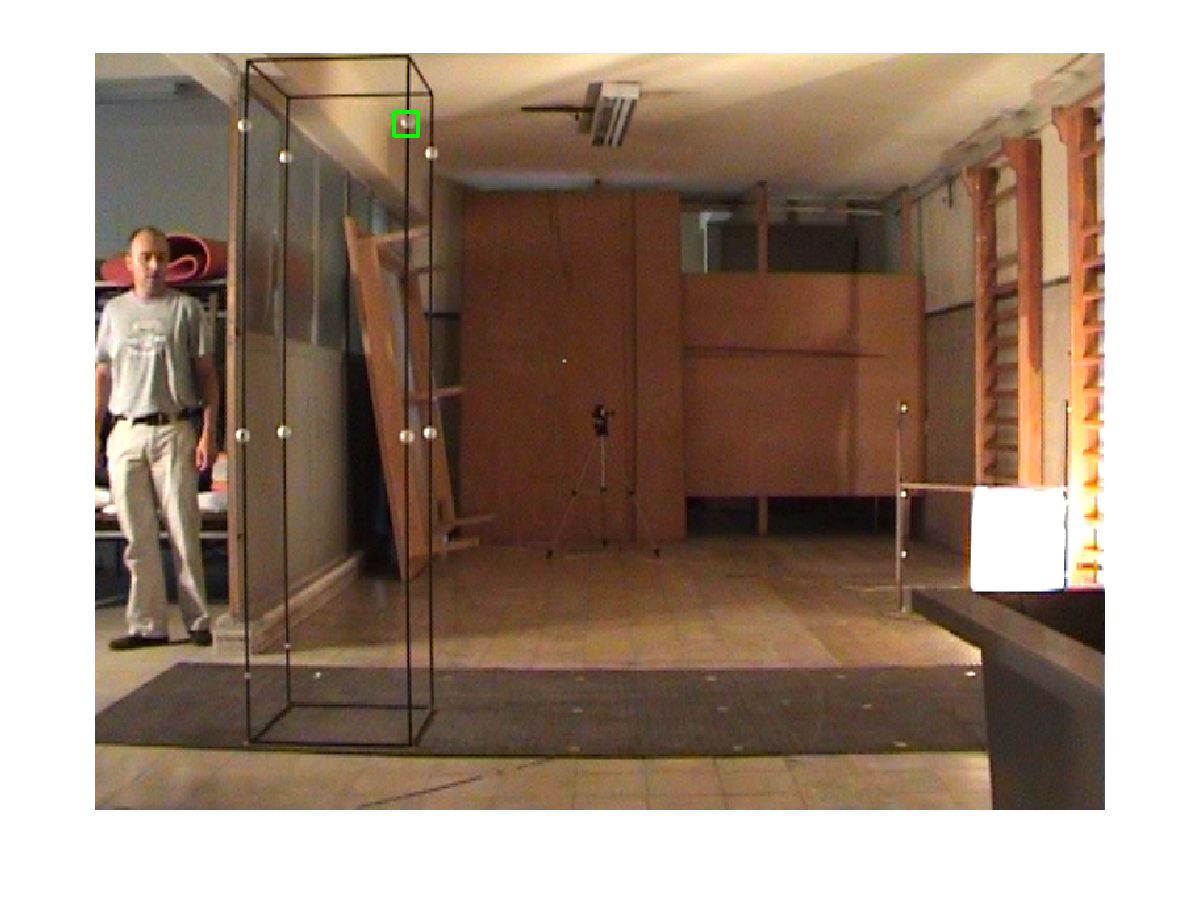
\includegraphics[trim = 32mm 0mm 68mm 0mm, clip,scale=0.45]{img/calibracion/calibrador_cam3.png}}
      
      \caption{Uno de los marcadores de calibrador seleccionado en cada una de las cámaras}
      \label{fig: vistas_calibrador}      
\end{figure}


Por otra parte la posición de los marcadores en el espacio 3D es conocida ya que se saben las medidas del calibrador, ver figura \ref{fig: medidas_calibrador}. Dichas posiciones pueden ser referidas un punto que puede elegirse arbitrariamente, así como los ejes de coordenadas $(x,y,z)$.

\begin{figure}[ht!]
        \centering
     {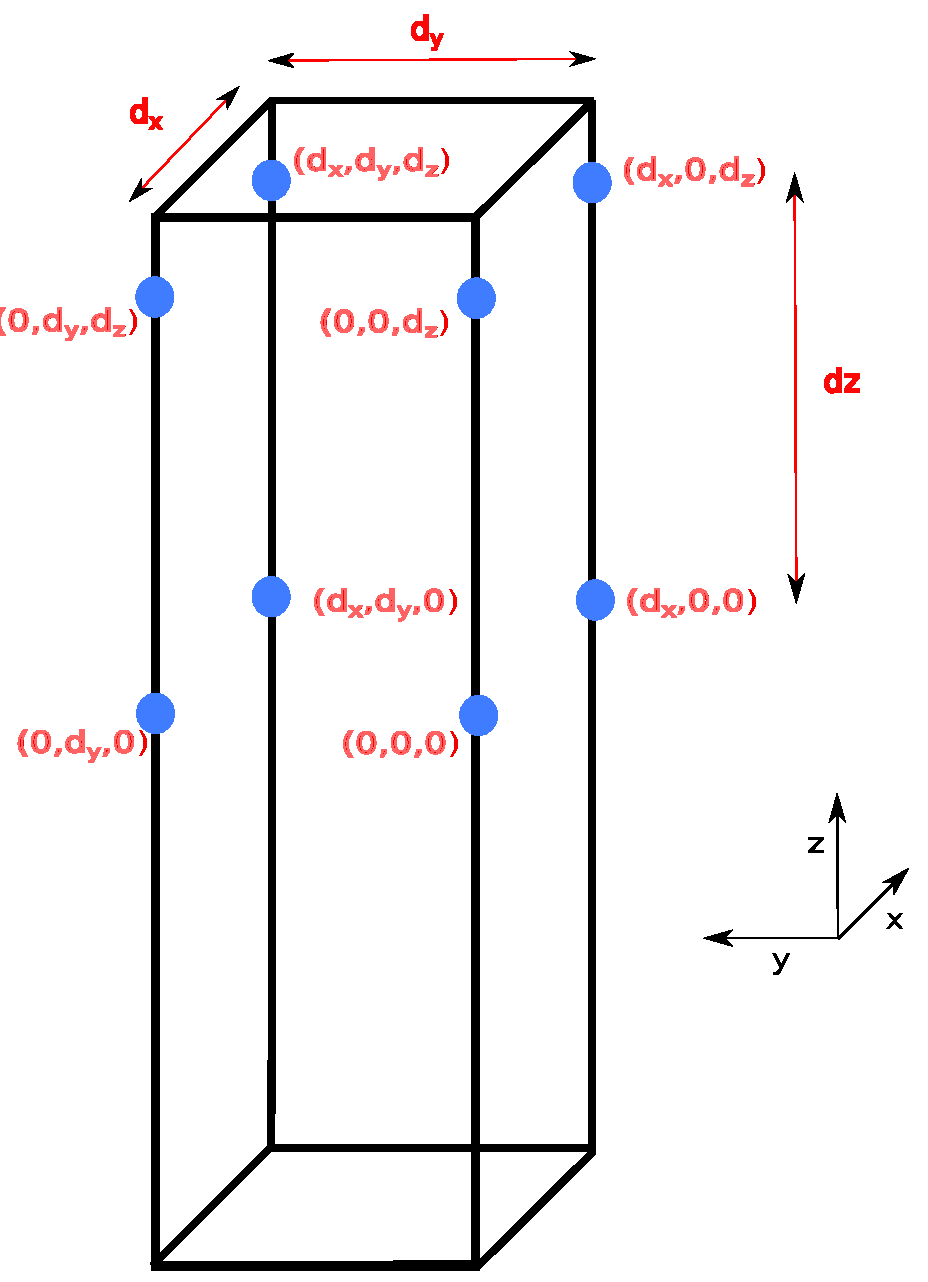
\includegraphics[scale=0.38]{img/calibracion/medidas_calibrador.pdf}}    
     \caption{Coordenadas de los marcadores del calibrador}
      \label{fig: medidas_calibrador}     
\end{figure}

   De esta forma se tiene asociados las coordenadas 3D de los marcadores en el espacio con sus correspondientes coordenadas 2D en píxeles en cada una de las cámaras, $X_i \leftrightarrow x_i$. Si se tiene una cantidad suficiente de puntos, entonces las matrices de proyección $P$ pueden ser estimadas tal que $x_i=PX_i$. Para esto se utiliza el algoritmo \textit{DLT}.\\
   
   Para cada asociación de puntos $X_i \leftrightarrow x_i$ se cumple que \cite{hartley}:
   
   \[
   \begin{pmatrix}
   0^T & -w_iX_i^T & y_iX_i^T \\
   w_iX_i^T & 0^T & -x_iX_i^T
   \end{pmatrix}
   \begin{pmatrix}
    P^1 \\
    P^2 \\
    P^3
   \end{pmatrix}
   = 0
   \]
   
 siendo $P^{iT}$ las columnas $i$-ésimas de $P$. Dicha matriz se obtiene resolviendo un conjunto de ecuaciones del tipo $Ap=0$.  Dado que por cada punto se tiene 2 ecuaciones y que la matriz $P$ tiene 12 entradas y 11 grados de libertad, ignorando el factor de escala, resulta que son necesarios conocer al menos 6 correspondencias $X_i \leftrightarrow x_i$.\\
 
 Tanto a los puntos imagen 2D como a los 3D se les aplica una normalización. Para los puntos 2D de cada vista se traslada el origen de coordenadas de dicha vista al centroide de los puntos y se aplica un escalado tal que la distancia promedio de los puntos al origen sea $\sqrt{2}$. Para los puntos 3D el mismo procedimiento excepto que el escalado que se aplica es tal que la distancia promedio al origen es $\sqrt{3}$. De esta manera se tiene dos matrices que realizan esta transformación, la matriz $T_{3D}$ tal que $\tilde{X_i} = T_{3D}^{}X_i$ para los puntos en el espacio, siendo $\tilde{X_i}$ los puntos normalizados. Análogamente para los 2D imagen se tiene la matriz $T_{2D}^{}$ tal que $\tilde{x_i} = T_{3D}^{}x_i$. \\
 
 Dado que las coordenadas de los puntos 2D están afectadas por el ruido y que se tienen más de 6 correspondencias $X_i \leftrightarrow x_i$ no existe una solución exacta a las ecuaciones $Ap=0$. Por lo tanto la solución se obtiene minimizando un error, en este se busca $p$ tal que minimice $||Ap||$. Para esto se utiliza la descomposición en valores singulares (SVD), donde se obtiene del vector singular asociado al menor valor singular. De esta manera se obtiene la matriz de proyección $\tilde{P}$. Por último debe descomponerse la normalización, por lo tanto la matriz de proyección $P = T_{2D}^{-1} \tilde{P} T_{3D}^{}$.
 
 \section{Calibración simulada en Blender}
 
 Con el objetivo de establecer una metodología que fuera válida para la configuración de cámaras con las que se diseño la base de datos, se probaron implementaciones existentes que pudieran calibrar dicha base de datos elaborada en Blender. Para esto se evaluó el siguiente toolbox elaborado en Matlab.\\ 
 
  \subsection{Toolbox Multi-Camera Self-Calibration.} 
 
 Este toolbox está especialmente pensado para la calibración simultánea de un conjunto de varias cámaras\footnote{\textcolor{blue}{\underline{http://cmp.felk.cvut.cz/~svoboda/SelfCal/}}. Accedido 3-12-14.}. El procedimiento consiste en capturar con todas las cámaras, el movimiento de una fuente puntual de luz que se mueve a lo largo de todo el volumen de trabajo. por tanto para cada cuadro se tiene un punto 3D en el espacio en una posición distinta y en cada una de las cámaras su correspondiente proyección si dicho punto es visible desde esa cámara. Para esto debe asegurarse que exista un contraste suficiente de la luz respecto al laboratorio. Puede usarse para esto, por ejemplo una lámpara led y que en el laboratorio exista poca o nula luz ambiente.\\
 
 
 Si se tienen $m$ cámaras y $n$ puntos 3D  
$\mathbf{X_j} = [X_j, Y_j, Z_j,1]^T$ con $j=1,\ldots,n$. La proyección de dichos puntos en los puntos imagen $u_j^i$:
\[ \lambda_j^i
\begin{bmatrix}
u_j^i \\
v_j^i \\
1
\end{bmatrix} 
 = \lambda_j^i u_j^i = P^i \mathbf{X_j}
\]

siendo $P^i$ la matriz de proyección de la $i$-ésima cámara y $u,v$ las coordenadas en píxeles de los puntos imagen. Las coordenadas de dichas proyecciones deben ser detectadas para cada cuadro y para cada cámara. El objetivo de la calibración es hallar los factores de escala $\lambda_j^i$ y las matrices de proyección $P^i$. Pueden expresarse todos los puntos y las matrices de proyección en una sola matriz $W_s$:

\[
W_s =
\begin{bmatrix}

	\lambda_1^1
	\begin{bmatrix}
	u_1^1 \\
	v_1^1 \\
	1
	\end{bmatrix} &
	
	\ldots &
	
	\lambda_n^1
	\begin{bmatrix}
	u_n^1 \\
	v_n^1 \\
	1
	\end{bmatrix} \\
	
	\vdots & \ddots & \vdots \\
	
	
	\lambda_1^m
	\begin{bmatrix}
	u_1^m \\
	v_1^m \\
	1
	\end{bmatrix} &
	
	\ldots &
	
	\lambda_n^m
	\begin{bmatrix}
	u_n^m \\
	v_n^m \\
	1
	\end{bmatrix} \\

\end{bmatrix}
= 
\begin{bmatrix}
P^1 \\
\vdots \\
P^m
\end{bmatrix}_{3m\text{x}4}
\quad
[\mathbf{X_1} \ldots \mathbf{X_n}]_{4\text{x}n}
\]
Por lo tanto se puede expresar:
\[ W_s = PX\]

donde $P = [P^1 \ldots P^m]^T$ y $X = [\mathbf{X_1} \ldots \mathbf{X_n}]$

Si son detectados una cantidad suficiente de puntos no ruidosos ($u_j^i, v_j^i$) y se conocen los $\lambda_j^i$, entonces $W_s$ tiene rango 4  y se puede factorizar en $P$ y $X$.\\

El número mínimo de cámaras para una correcta calibración depende del número de parámetros conocidos de las cámaras o del número de parámetros que se conocen pero son los mismos para todas las cámaras. 3 cámaras son suficientes si se conocen todos los puntos principales o si los parámetros internos de las cámaras no se conocen pero son los mismo para todas ellas.\\

La simulación en Blender se logra creando un punto 3D que toma para cada cuadro distintas posiciones en forma aleatoria dentro del volumen de trabajo. Para cada cuadro se \textit{renderiza} su posición en las 17 cámaras. En este caso se han tomado 500 posiciones distintas. En la figura \ref{fig: blender toolbox laser} se muestra en Blender la distintas posiciones que toma en un punto dentro del volumen de trabajo.

\begin{figure}[ht!]
\begin{center}
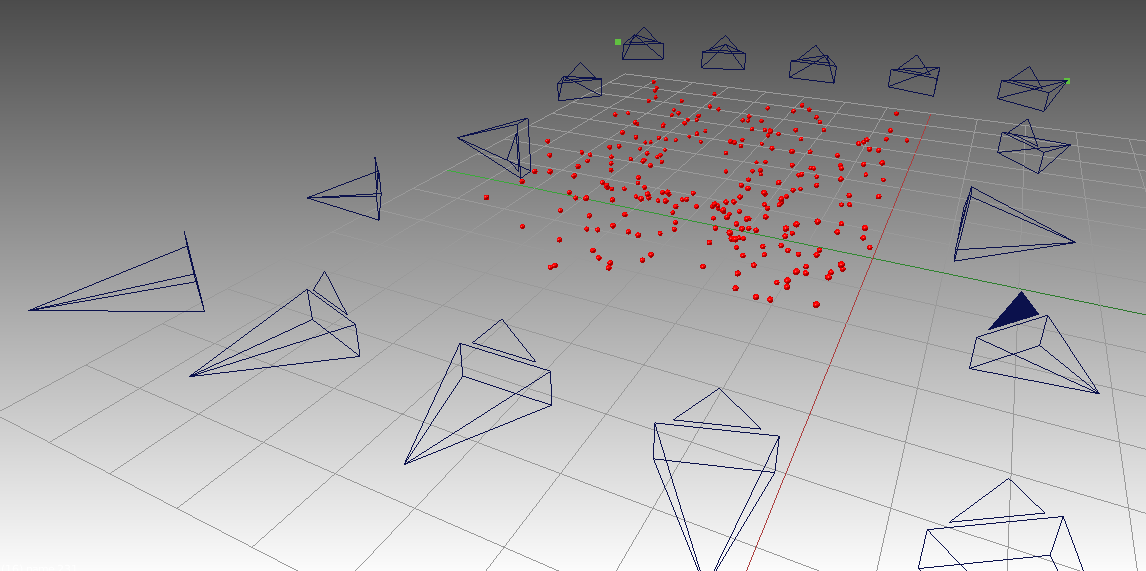
\includegraphics[scale=0.22]{img/calibracion/blender_toolbox_laser.png}
\end{center}
\caption{Posiciones de un punto 3D dentro del volumen de trabajo}
\label{fig: blender toolbox laser}
\end{figure}

En la figura \ref{fig: camaras blender} se muestra la configuración de las 17 cámaras en el espacio 3D de Blender. En la figura \ref{fig: camaras calibracion} se muestra, con círculos en azul, la posición de las cámaras obtenidas del resultado de la calibración. Se observa además, en rojo, la reconstrucción de las posiciones del punto 3D en el espacio.


\begin{figure}[ht!]
        \hspace{-1cm}
        \subfloat[Blender]{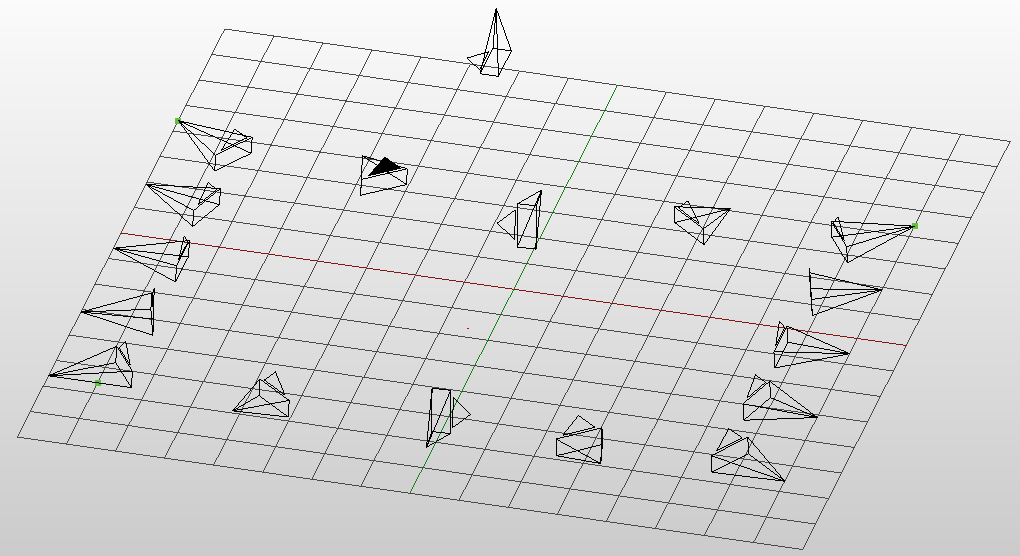
\includegraphics[trim = 0mm 0mm 0mm 0mm, clip,scale=0.24]{img/calibracion/camaras_blender.png}\label{fig: camaras blender}}
                \hspace{0.01cm}                
        \subfloat[Calibración]{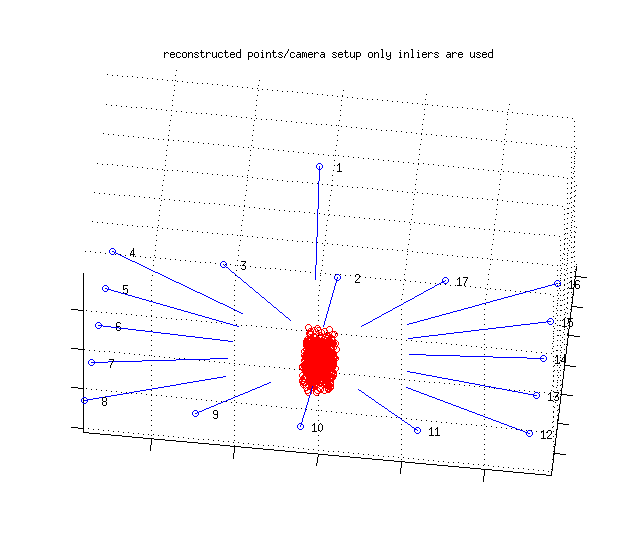
\includegraphics[trim = 0mm 20mm 10mm 20mm, clip,scale=0.46]{img/calibracion/camaras_calibracion.png}\label{fig: camaras calibracion}}
        
      
      \caption{Configuración de las cámaras en el espacio 3D de Blender y la misma configuración hallada mediante la calibración}
      \label{fig: configuracion camaras}
      
\end{figure}

En la figura \ref{fig: error reproyeccion} se muestra e promedio y la desviación del error de re-proyección estándar obtenido para cada una de las cámaras.

\begin{figure}[ht!]
\begin{center}
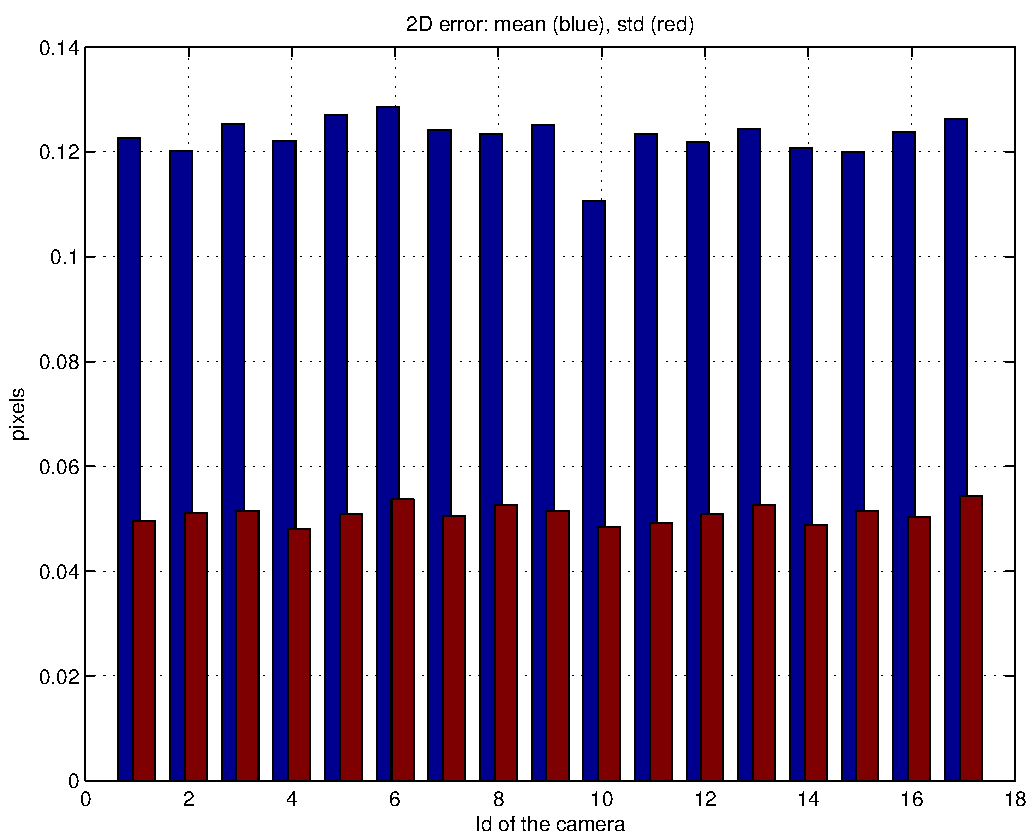
\includegraphics[scale=0.4]{img/calibracion/reprerrors.pdf}
\end{center}

\caption{Promedio y desviación  del error de re-proyección en todas las cámaras }
\label{fig: error reproyeccion}
\end{figure}
  







\subsection{Markers Detection}
Markers detection block, can be divided in two parts: \textit{segmentation} and \textit{objects filter}.
%
Algorithm makes the detection through the following process:
%
\begin{enumerate}
  \item Get each frame from video input.
  \item Take a frame and segment it using Otsu's threshold.
  \item Detect markers from segmented image.
  \item Write detected markers position in an XML file.
  %\item Se escribe la posición de los marcadores detectados para este cuadro en un archivo con formato XML.
  \item Take the following frame and repeat process from step two.
\end{enumerate}
%
\subsubsection{Detection stages description}
\textit{Segmentation} block uses thresholds with three class Otsu's method\cite{otsu}.\\
%
\textit{Filtering} stage is just a classification of segmented objects. Since objects to be detected have relatively simple shapes (white circles on dark background) and laboratory conditions are controlled during the capture, this stage not required to implement a complex algorithm. Particularly, it was implemented a circular object detector based on geometric moments\cite{imageMoments} and an area based filter.
%
\subsubsection{Results}
It was observed that results on segmentation stage strongly depends from capture conditions and calculated threshold. Special care must be taken in capture conditions since if not meet the established, results are not entirely satisfactory.
On the other hand, if captures are made in the established conditions, obtained results are acceptable (Figure \ref{ejemploabelumbr2}).
\vspace{-0.5cm}
\begin{figure}[ht!]
      \centering
        {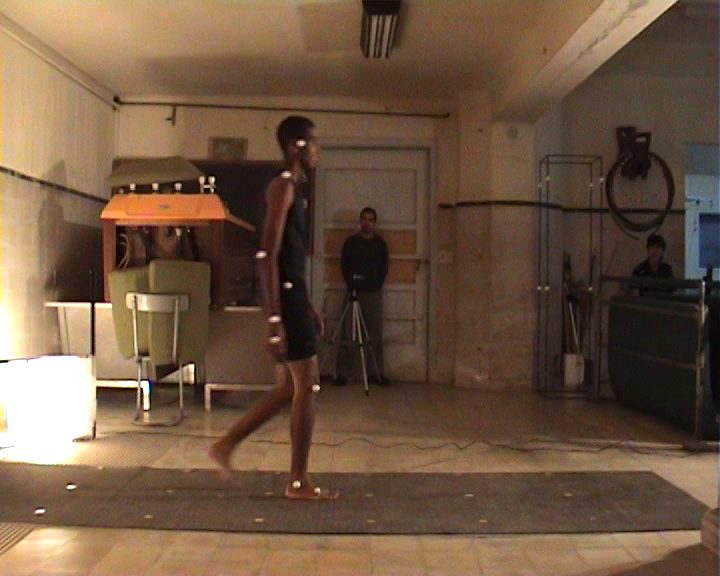
\includegraphics[scale=0.10]{imagenes/abel_original_video.png}\label{abelvideo}}\hspace{1 mm}
        {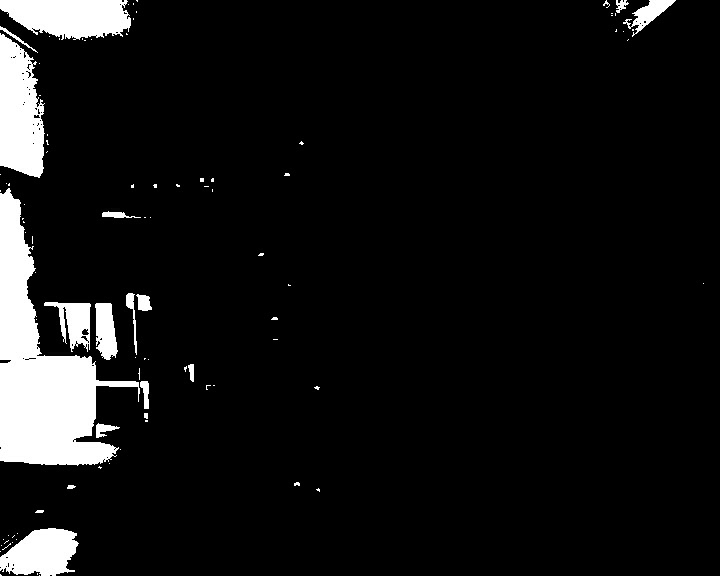
\includegraphics[scale=0.10]{imagenes/abel_original_filtro.png}\label{abelfiltro}}
        {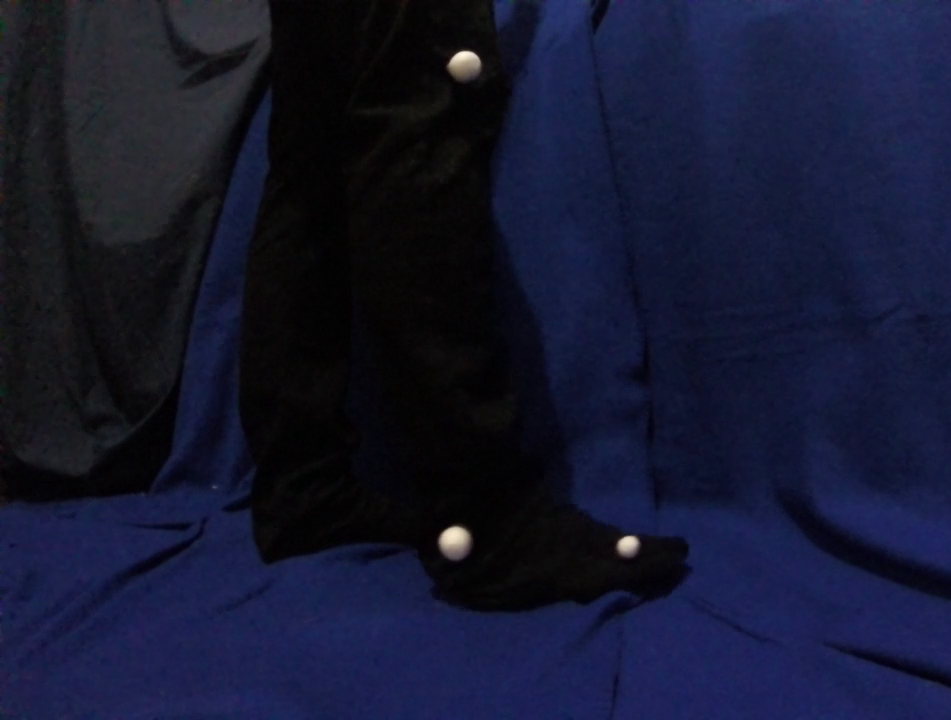
\includegraphics[scale=0.07]{imagenes/orig.png}\label{abelvideo2}}\hspace{1 mm}
       % {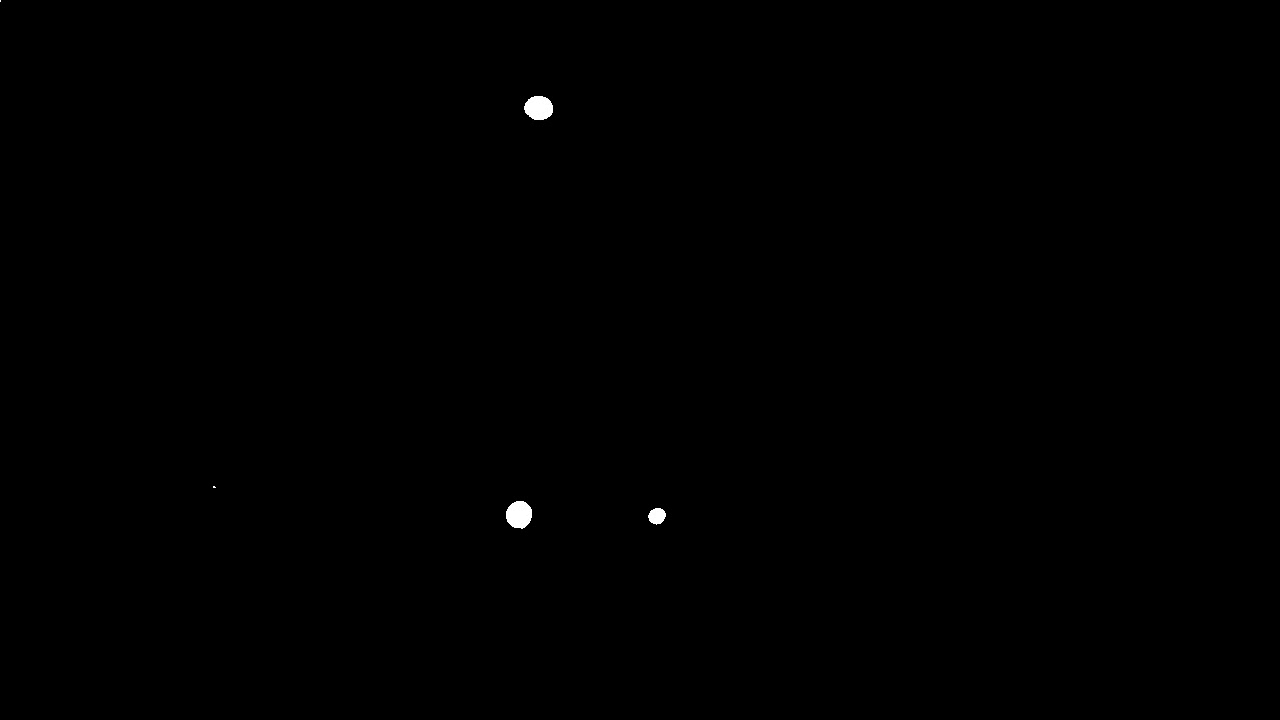
\includegraphics[scale=0.07]{imagenes/filtr.png}\label{abelfiltro2}}\hspace{1 mm}
        {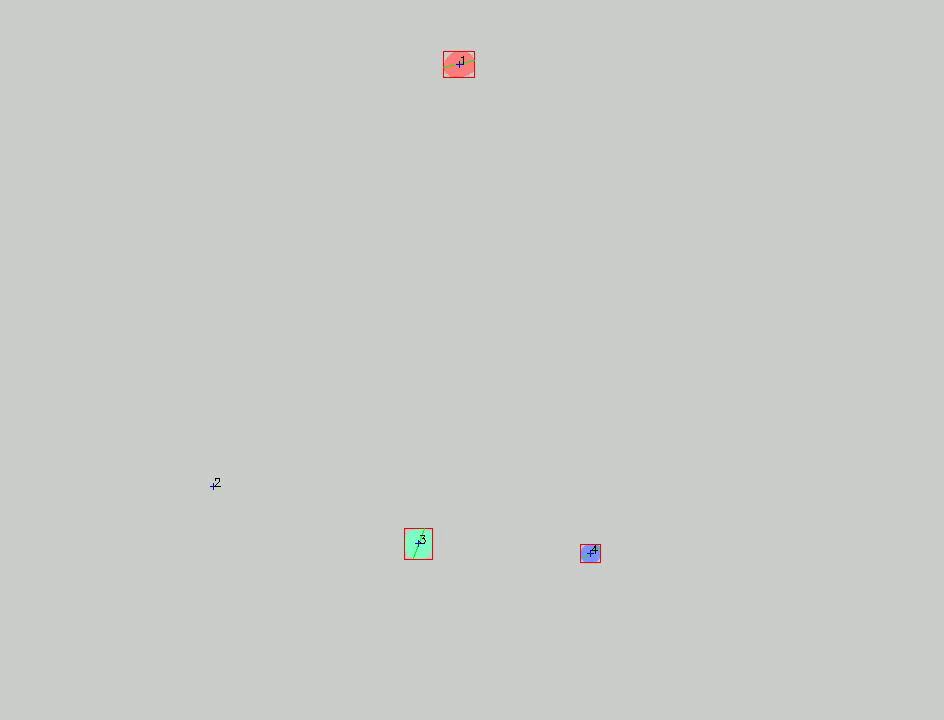
\includegraphics[scale=0.07]{imagenes/detect.png}
        \label{abeldetect}}
      \caption{%Entradas y salidas de cada etapa del bloque de deteción.
       %\textbf{(\ref{abelvideo})} 
       \textit{Left}: original image from a sequencue without capture hypothesis. 
       \textit{Left center}: segmentation results without capture hypothesis.
       % \textbf{(\ref{abelvideo2})} 
       \textit{Right center}: Original capture from a real sequence under capture hypothesis.
       % \textbf{(\ref{abelfiltro2})} Imagen filtrada con el umbral de Otsu. \textbf{(\ref{abeldetect})}
       \textit{Right}: Detected markers.}  
      \label{ejemploabelumbr2}
\end{figure}
%\vspace{-0.6cm}
%\vspace{-0.8cm} % % % % % % % % % % % % % % % % % % % % % % % % % % % % % %
\chapter{Reconstrucción}\label{reconstruccion}

\section{Introducción}
A la salida del bloque de detección de marcadores se tiene, para cada cámara y para cada cuadro de una secuencia adquirida, un conjunto de coordenadas en dos dimensiones $(x,y)$ que ubican la posición en la imagen de aquellos marcadores que fueron detectados.
El proceso de reconstrucción consiste en obtener las coordenadas en tres dimensiones de la posición de los marcadores en el espacio a partir de las coordenadas en dos dimensiones obtenidas en el bloque anterior.
En la Figura \ref{fig: esquema_reconstruccion} se muestra un bosquejo de la reconstrucción de un marcador usando para esto la detección de marcadores en dos cámaras.\\

\begin{figure}[ht!]
\begin{center}
%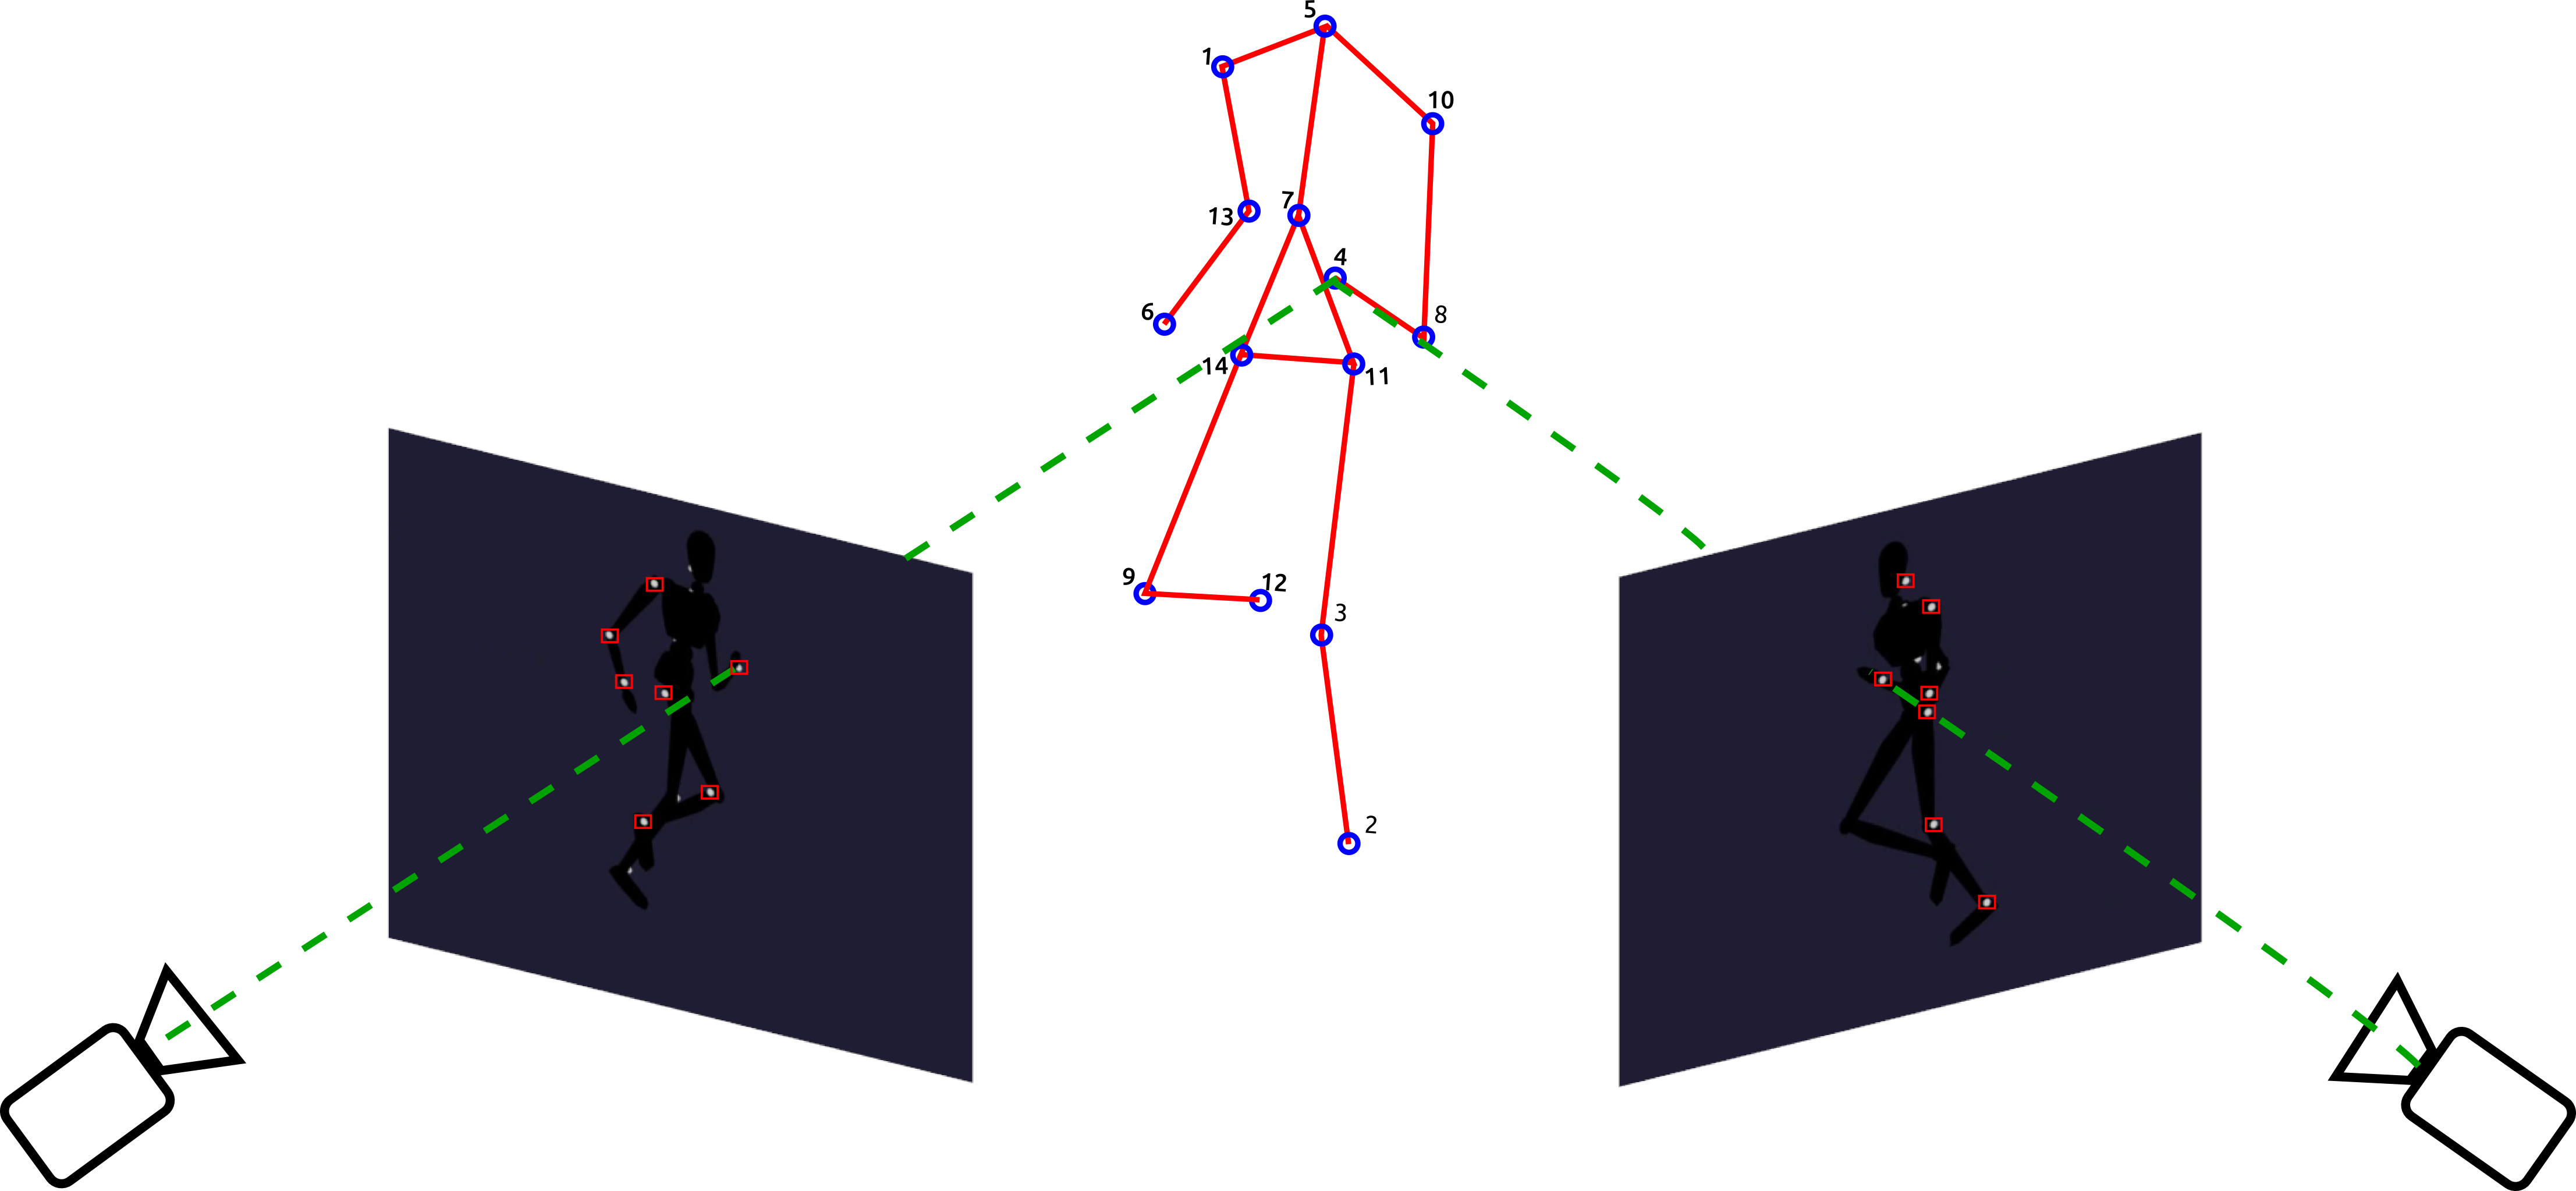
\includegraphics[scale=0.20]{img/Reconstruccion/ejemplo_reconstruccion.png}
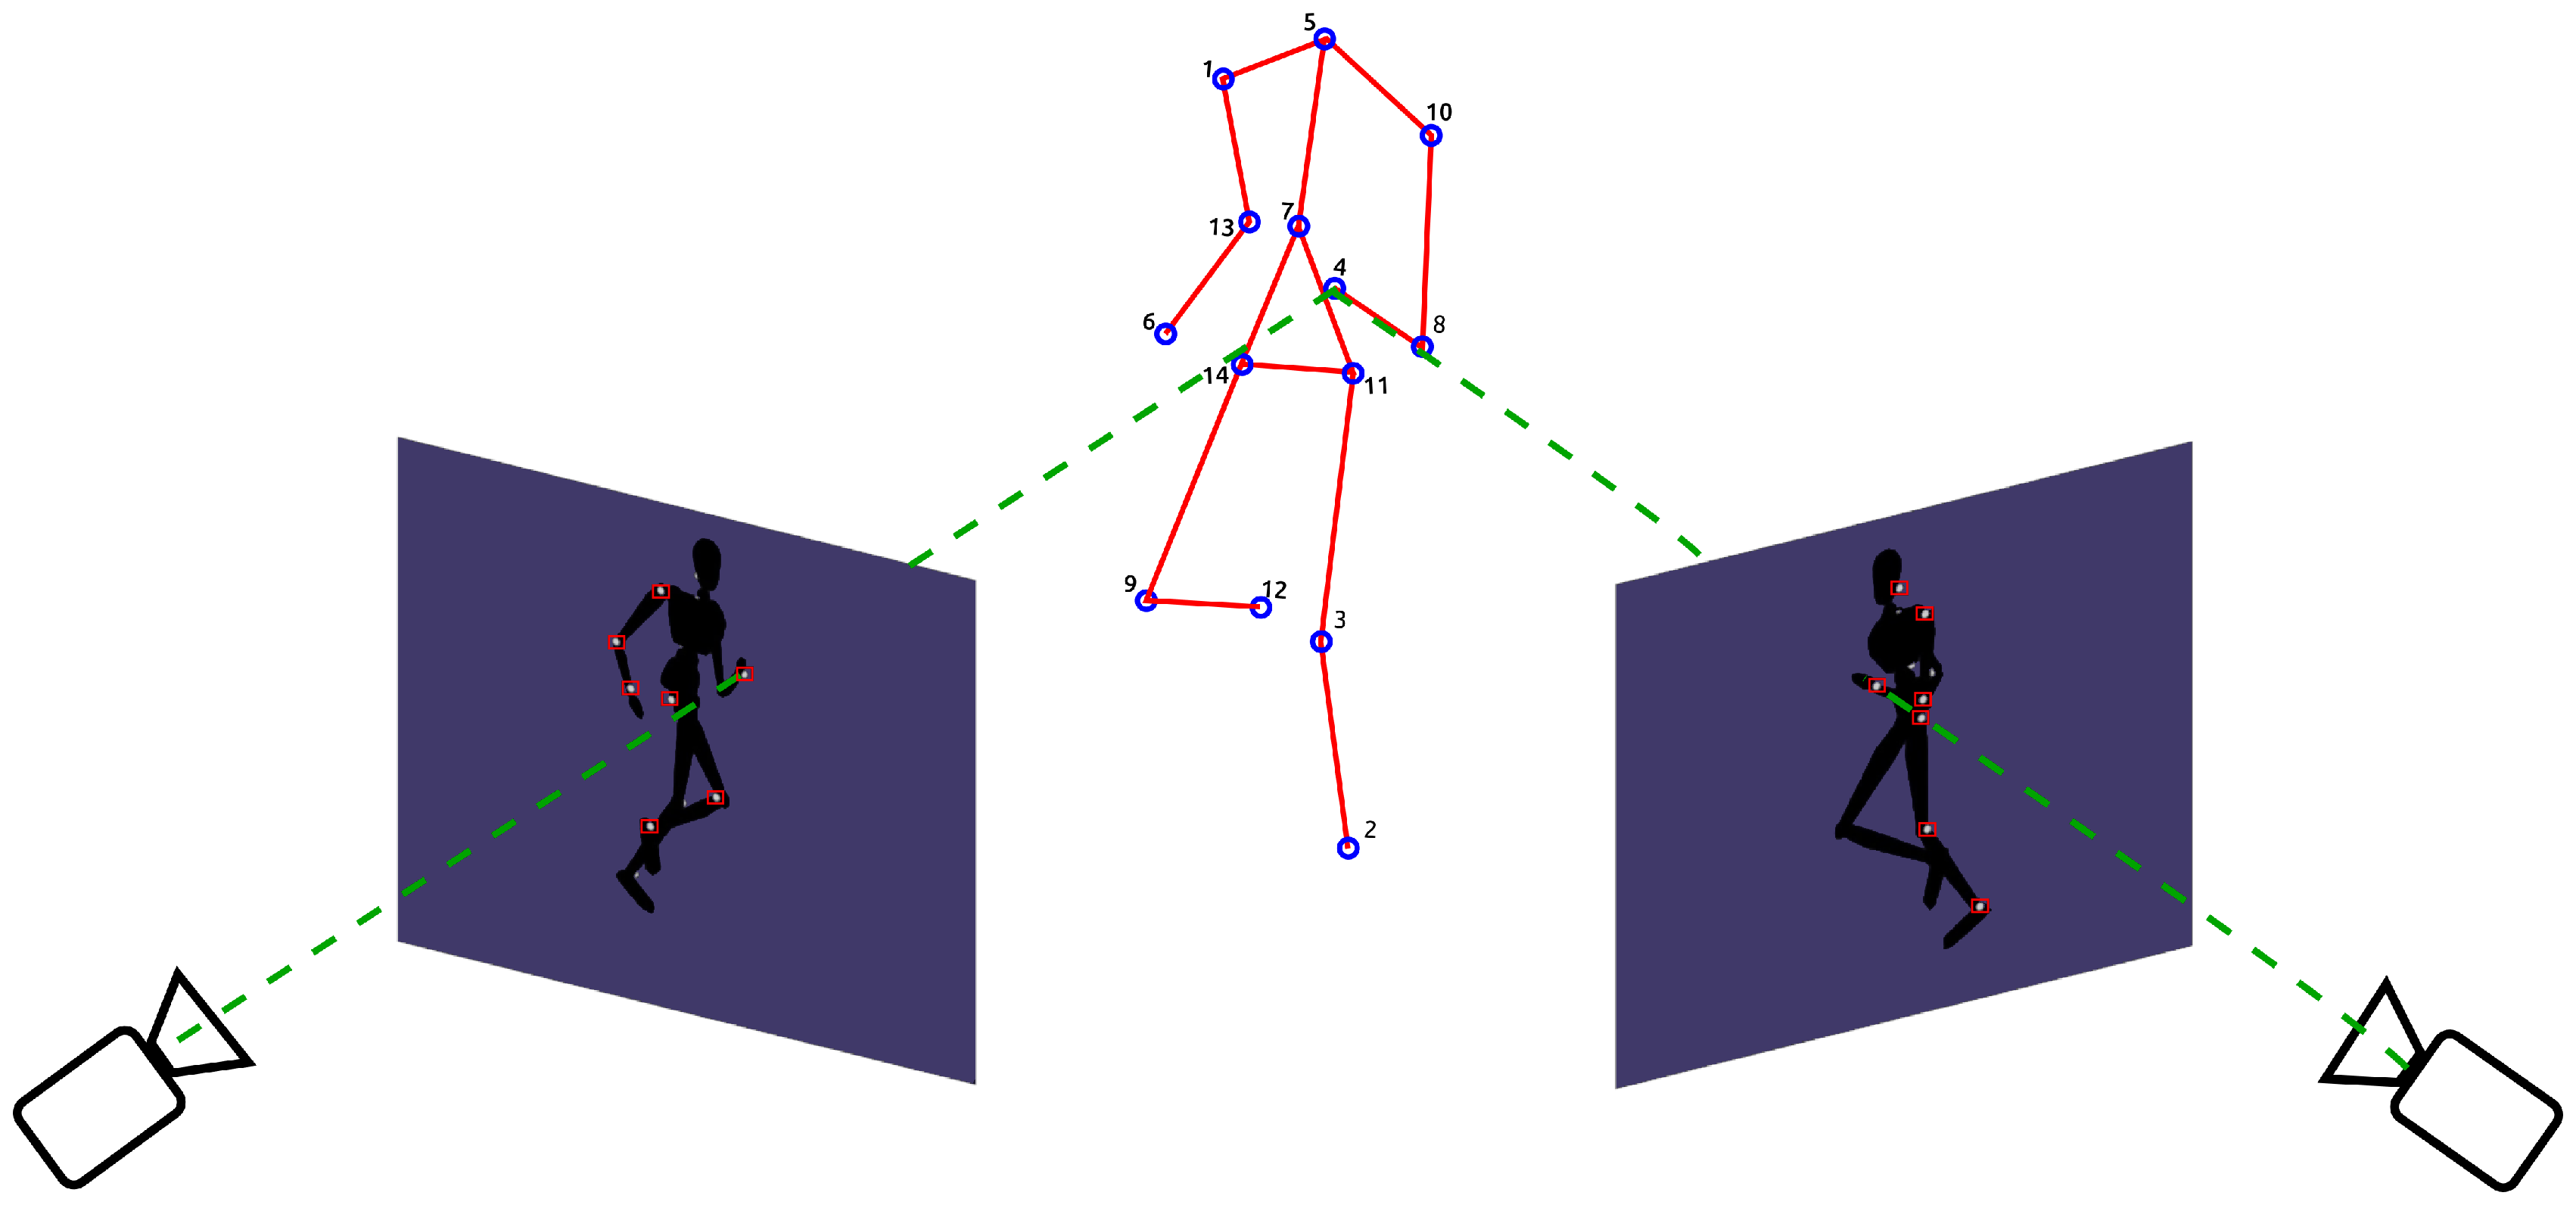
\includegraphics[scale=0.20]{img/Reconstruccion/reconstruccion}
\end{center}
\caption{Reconstrucción con dos cámaras.}
\label{fig: esquema_reconstruccion}
\end{figure}

%Se observa en la figura a uno de los marcadores detectados desde las dos vistas y su correspondiente punto 3D reconstruido.\\
El proceso de reconstrucción implementado fue inspirado en el trabajo de Herda \cite{herda} y consiste en tres pasos fundamentales:
\begin{enumerate}
\item Determinar aquellos marcadores detectados en las distintas cámaras que corresponden a un mismo marcador en el espacio. De esta manera se establece una correspondencia entre los marcadores detectados en las distintas vistas. Dichas asociaciones se establecen de a pares de cámaras.
\item Una vez establecidas estas correspondencias se selecciona aquella que bajo algún criterio, pueda considerarse con mayores posibilidades de ser una asociación correcta. Luego se determina la posición en el espacio del marcador a partir de la asociación seleccionada.
\item Una vez reconstruido uno de los marcadores debe verificarse si dicho marcador fue detectado en el resto de las cámaras.
\end{enumerate}


\section{Geometría epipolar}



Para explicar el algoritmo de reconstrucción es necesario describir brevemente algunos conceptos fundamentales de la geometría epipolar.  Dicha geometría es la que se presenta cuando dos cámaras en distintas posiciones se encuentran capturando el mismo espacio 3D. El análisis de esta situación permite obtener relaciones entre los puntos 3D con sus correspondientes proyecciones en las cámaras, así como las relaciones entre los propios puntos proyectados en las distintas cámaras\cite{cyganek}\cite{hartley}. \\


 Como se muestra en la Figura \ref{fig: geometria_epipolar}, se tiene el caso en que dos cámaras observan un mismo punto 3D en el espacio, el punto $X$. Para esto se considera el modelo \textit{pinhole} de la cámara  descrito en el Capítulo \ref{calibracion}. En ese caso los puntos $O_1$ y $O_2$ son los centros o focos de las cámaras.\\
 
 \begin{figure}[ht!]
 \begin{center}
 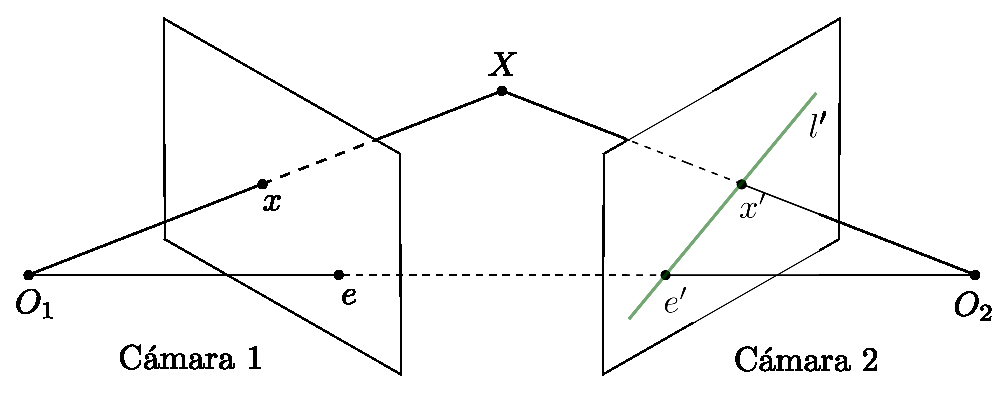
\includegraphics[scale=0.7]{img/Reconstruccion/geometria_epipolar}
 \end{center}
 \caption{Geometría epipolar.}
 \label{fig: geometria_epipolar}
 \end{figure}
 
  El punto $X$ se proyecta en dichas cámaras en los puntos $x$ y $x'$. Es decir, $x$ pertenece a la intersección de la retina de la cámara 1, con el rayo de proyección $\overline{O_1X}$. Análogamente el punto $x'$ pertenece a la intersección de la retina de la cámara 2 con el rayo de proyección $\overline{O_2X}$. A su vez, los focos de ambas cámaras $O_1$ y $O_2$ definen un rayo que corta a las retinas de las cámaras en los puntos $e$ y $e'$ llamados epipolos.\\
  
  Si el punto $X$ varía sobre el espacio 3D, se tienen múltiples rayos de proyección que pasan por dicho punto y el foco de la cámara 1, el punto $O_1$. Dado que $O_1$ se proyecta en la cámara 2 como el punto $e'$ en el plano imagen, todas los rayos  $\overline{O_1X}$ se proyectan en dicha cámara como rectas que se intersecan en el punto $e'$, a estas rectas se les denomina rectas epipolares. Análogamente los sucesivos rayos de proyección $\overline{O_2X}$ se proyectan sobre la cámara 1 como rectas epipolares que se intersecan en el punto $e$. De esta manera se tiene que los puntos $X$, $O_1$ y $O_2$ forman un plano, llamado plano epipolar,  que interseca a los planos imagen en las rectas epipolares.\\
  
De lo anterior se observa que teniendo la proyección $x$ de un punto $X$ sobre la cámara 1, también se conoce la recta epipolar $l'$ y se puede ver que el punto $X$ se proyecta en la cámara 2 en un punto $x'$ situado en dicha recta epipolar $l'=\overline{e'x'}$. Esto implica que por cada punto visto en una retina en la otra se observa una línea.\\
 
Si los puntos $x$ y $x'$ son conocidos, sus rayos de proyección son también conocidos y si estos puntos corresponden a un mismo punto 3D sus rayos de proyección deben interceptarse en $X$. Por lo tanto las coordenadas del punto X pueden derivarse a partir de las coordenadas de sus puntos imagen.\\
 
Para el caso de cámaras reales se tienen distorsiones de ruido, imperfecciones en las lentes de las cámaras, etc. que producen que las proyecciones sean tal que el punto 3D, su proyección en la cámara y el foco de la misma no sean colineales, por lo tanto la proyección real de un punto 3D va a ser aproximadamente el punto ideal de su proyección. \\

\subsection{Matriz Fundamental}

La matriz fundamental es la representación algebraica de la geometría epipolar. Si se tiene el punto $X$ y sus correspondientes proyecciones $x$ y $x'$ en las cámaras, se verifica la siguiente condición :

\begin{equation}
(x')^T F x = 0
\label{ec: matriz fundamental}
\end{equation}
siendo  $F$ la matriz fundamental y $x$, $x'$ las proyecciones en coordenadas homogéneas.\\

Supongamos que se tienen para la cámara 1, la matriz de proyección $P$ y el punto $x$ mencionado anteriormente. El rayo de proyección $\overline{O_1X}$  puede describirse en forma paramétrica como:

\begin{equation}
	X(\lambda) = P^+x+\lambda O_1
\end{equation}

\hspace{-0.6cm}donde $P^+$ es la pseudo-inversa de $P$, tal que $PP^+=I$.\
En particular se toman dos puntos de esa recta, el punto $P^+x$ ($\lambda = 0$) y el punto $O_1$ ($\lambda = \infty$).\
Si se proyectan estos puntos en la cámara 2 se obtienen los puntos $P'P^+x$ y $P'O_1$ respectivamente, siendo $P'$ la matriz de proyección de la cámara 2. Estos puntos pertenecen a la recta epipolar:

\begin{equation}
l' = (P'O_1) \times (P'P^+ x)
\end{equation}

El punto $P'O_1$ es el epipolo $e'$ de la cámara 2. Por lo tanto se tiene que\\$l' = e' \times (P'P^+) x$, donde se define la matriz fundamental como:

\begin{equation}
F=e' \times P'P^+
\end{equation}

Si los puntos imagen se corresponden $x \leftrightarrow x'$, entonces $x'$ se encuentra en la recta epipolar $l'=Fx$ correspondiente al punto $x$, lo cual implica que se cumple $0=(x')^Tl'$ y por lo tanto se verifica la condición de la Ecuación \ref{ec: matriz fundamental}. 

Como se explica anteriormente las igualdades de las ecuaciones mostradas se cumplen en condiciones ideales pero no para cámaras reales en las que aparecen los efectos del ruido, etc., por lo tanto cabe esperar que si se tiene un punto $x$ y su correspondiente $x'$, la Ecuación \ref{ec: matriz fundamental} no se verifique exactamente, aunque si debe devolver un valor próximo a cero.\\

Una propiedad básica de esta matriz es que si $F$ es la matriz fundamental del par de cámaras con matrices de proyección ($P,P'$), entonces $F^T$ es la matriz fundamental del par de cámaras en sentido opuesto: ($P',P$). Por otra parte si se tiene el punto $x$ en la imagen de una cámara, su recta epipolar correspondiente en otra cámara es $l'=Fx$. Análogamente $l=F^Tx'$ representa la línea epipolar asociada con $x'$ en la segunda cámara.

\section{Algoritmo propuesto por Herda }

Como se explica en el Capítulo \ref{sec:implementacion_bloques_sistema}, se inicia la implementación de este bloque a partir del algoritmo propuesto por Herda \cite{herda}. Este algoritmo en algunos aspectos no es descripto con el detalle suficiente tal que pueda ser replicado fielmente. Por esta razón su implementación se ha elaborado realizando algunos supuestos en los casos donde su interpretación presenta ambigüedades.\\

Por otra parte, el sistema diseñado por Lorna Herda pretende utilizar la información del esqueleto (ver Capítulo \ref{sec:implementacion_bloques_sistema}), como por ejemplo la posición de articulaciones, distancias entre marcadores, etc. Dado que esta etapa del algoritmo no fue implementada resultó necesario robustecer el proceso de reconstrucción en las partes del algoritmo donde no se utiliza esta información.\\


Además, este algoritmo utiliza la triangulación estéreo para reconstruir un punto 3D a partir de los puntos 2D detectados en las distintas vistas. La correspondencia entre distintas vistas se establece mediante la matriz fundamental, cuyos conceptos fueron explicados en la sección anterior. Esta matriz se puede obtener luego del proceso de calibración.\\

Las ideas que sigue el algoritmo se describen a continuación:\

\begin{itemize}
\item Se toman dos vistas y se realiza el test de la condición epipolar (Sección \ref{MejorAsociacion}). Si existe una asociación no ambigua se reconstruyen  las coordenadas 3D a partir de las coordenadas 2D.

\item Las coordenadas 3D reconstruidas se re-proyectan en las cámaras restantes. Los puntos 2D encontrados en esa re-proyección son asociados al punto 3D. De esta forma se tiene por cada punto 3D, sus correspondientes puntos 2D asociados en las distintas vistas.\

\item Se considera que un marcador 3D está correctamente reconstruido si se re-proyecta en al menos una cámara. A este tipo de reconstrucción se le llama \textit{reconstrucción trinocular}.

\item Si el número de marcadores reconstruidos es inferior al número de marcadores colocados sobre la persona, entonces se realiza una segunda asociación entre dos vistas. En este caso la reconstrucción se realiza solamente con dos vistas (\textit{reconstrucción binocular}).\\

\end{itemize}

Posteriormente el algoritmo plantea realizar ciertos chequeos sobre los puntos reconstruidos de manera de validarlos. Dichos chequeos utilizan información del esqueleto (Figura \ref{fig:oclusion_herda}).


Lo que se busca verificar en dichos chequeos, es que para un determinado cuadro los marcadores sean efectivamente visibles por aquellas cámaras que los reconstruyeron y no están ocultos por alguna parte del cuerpo, lo que evidenciaría que la reconstrucción es incorrecta. Si esto llegara a suceder, el algoritmo busca otras vistas de las cuales reconstruir el marcador.

\begin{figure}[ht!]
 \begin{center}
 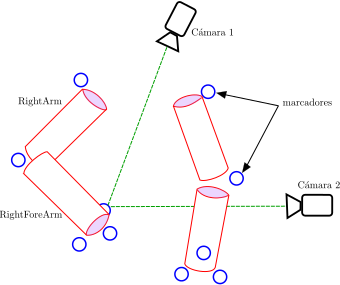
\includegraphics[scale=0.8]{img/Reconstruccion/oclusion_herda}
 \end{center}
 \caption{Chequeo de visibilidad y oclusión \cite{herda}.}
 \label{fig:oclusion_herda}
 \end{figure}


\section{Algoritmo implementado}

En la Sección anterior se describió el algoritmo de reconstrucción propuesto en el sistema de Herda, sin embargo, el algoritmo implementado no es exactamente el mismo. Como se aclara sobre el final de la Sección \ref{sec:implementacion_bloques_sistema} , la cantidad de módulos a implementar es grande, presentando ambigüedades importantes que dificultan en muchos casos su reproducibilidad, considerando los tiempos con los que cuenta el proyecto, se decide dar prioridad a los bloques principales, comenzando por lo básico e implementando módulos hasta lograr la performance necesaria. A continuación se describe la implementación realizada para este proyecto y las diferencias con el algoritmo de reconstrucción propuesto por Herda.\\

El algoritmo implementado recibe como entrada los puntos 2D de los marcadores detectados y devuelve como salida los puntos 3D reconstruidos. El primer paso consiste en establecer una asociación entre ciertos puntos 2D de distintas cámaras. Luego, se pasa a un conjunto de bloques que se ejecutan de manera iterativa hasta que no queden marcadores para reconstruir. En dicho bloque se busca la mejor asociación entre puntos, bajo determinado criterio, luego se reconstruye un punto 3D y se realiza un proceso de validación de dicha reconstrucción. En la iteración siguiente se actualizan las asociaciones que habían sido establecidas previamente. Cuando no hay más marcadores para reconstruir se detiene el proceso iterativo y se devuelven aquellos marcadores que fueron reconstruidos en cada iteración. En la Figura \ref{fig: diagrama algoritmo} se presenta un diagrama del algoritmo.\\

\begin{figure}[ht!]
\hspace{-1cm}
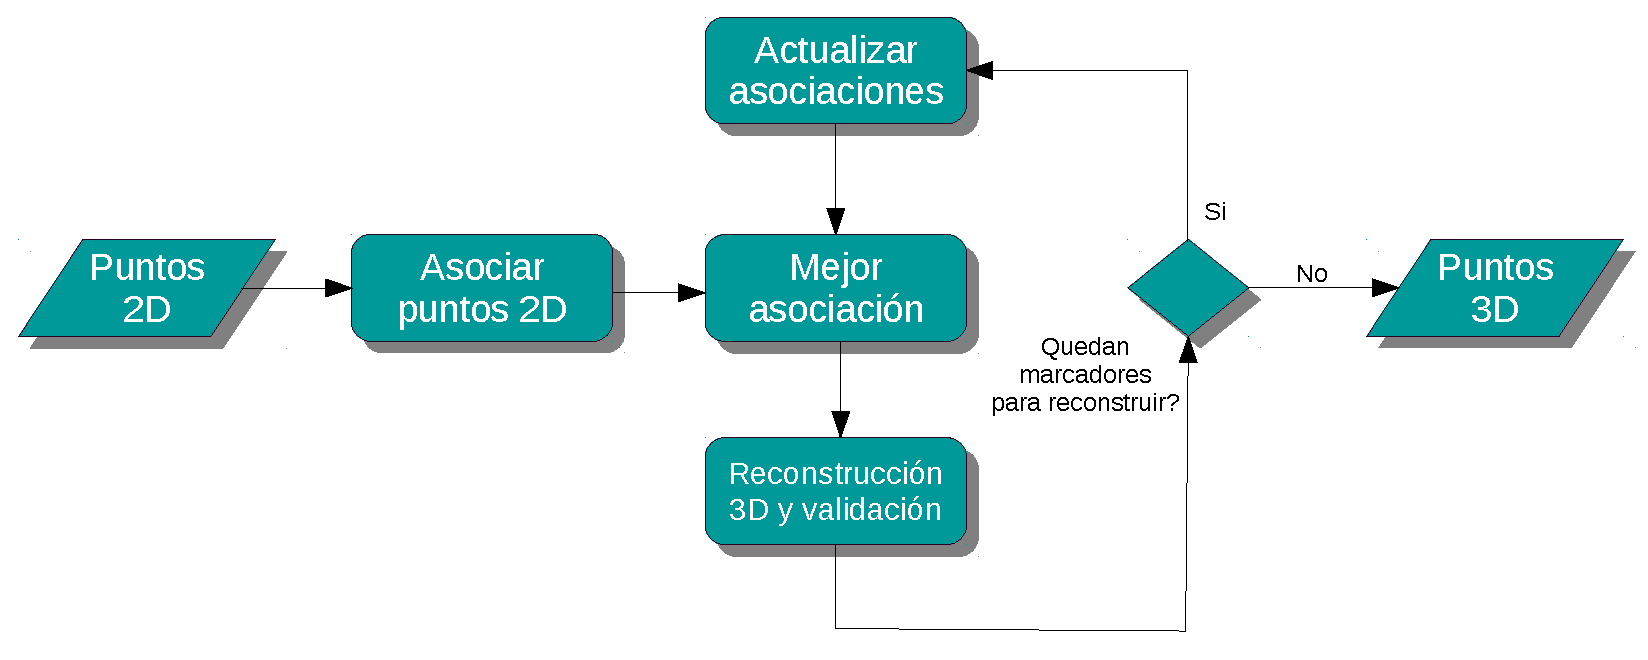
\includegraphics[scale=0.55]{img/Reconstruccion/diagrama_algoritmo.pdf}
\caption{Diagrama del algoritmo implementado.}
\label{fig: diagrama algoritmo}
\end{figure}

A continuación se describe el funcionamiento de cada uno de los bloques.

\subsection{Asociar puntos 2D}\label{seccion_asociar2D_uno}

Este bloque recibe como entrada las coordenadas de los puntos detectados en cada una de las cámaras, parámetros de las mismas tales como sus matrices de proyección y devuelve para cada punto una lista ordenada por relevancia, de las asociaciones existentes con puntos en otras cámaras.
Basándose en lo explicado anteriormente el proceso  se puede ejemplificar  en la Figura \ref{fig: cam2cam }.

\begin{figure}[ht!]
\hspace{0.3cm}
\includegraphics[scale=0.7]{img/Reconstruccion/cam2cam2}
\caption{Asociación de puntos 2D en dos cámaras.}
\label{fig: cam2cam }
\end{figure}

En primer lugar se seleccionan dos cámaras y se considera un punto en una de ellas, por ejemplo el punto $x_{11}$ de la cámara 1, y se evalúa la Ecuación \ref{ec: matriz fundamental} para cada punto en la cámara 2. Esto equivale a proyectar la recta epipolar $l'$ correspondiente al punto $x_{11}$ sobre la cámara 2  y tomar las distancias de los puntos detectados en la cámara 2 a la recta $l'$. Se demuestra que dicha distancia difiere a menos de un factor de escala respecto al valor obtenido al evaluar la Ecuación \ref{ec: matriz fundamental}. Se asume que los puntos de la cámara 2 que tengan mayor posibilidad de corresponder con el punto $x_{11}$, son aquellos que al ser evaluados por la ecuación obtienen valores próximos a cero.
De esta manera se obtiene para cada punto en la cámara 1 un conjunto de puntos en la cámara 2 ordenados según su distancia a la recta epipolar correspondiente.
Repitiendo el procedimiento de manera inversa, esto es, de la cámara 2 a la cámara 1, se obtiene igualmente para cada punto de la cámara 2  los puntos de la cámara 1 ordenados según su proximidad a la recta epipolar correspondiente. A continuación se toman otros pares de cámaras y se vuelve a repetir el proceso. 

Es importante resaltar que para la elección de los pares de cámaras se han considerado dos casos.
El primero de ellos evalúa cada cámara respecto a todas las restantes y el segundo considera la disposición de las cámaras en el espacio y empareja las cámaras adyacentes de manera consecutiva (ver Figura \ref{img_asociacion}). %Más adelante se demuestra que este segundo procedimiento da mejores resultados.ACÁ SE DEBE REFERENCIAR BIEN DONDE ESTA ESA DEMOSTRACIÓN \\

 \begin{figure}[ht!]
   \centering 
    \subfloat[Cada cámara con las restantes. Ejemplo de emparejamiento de la cámara 1.]{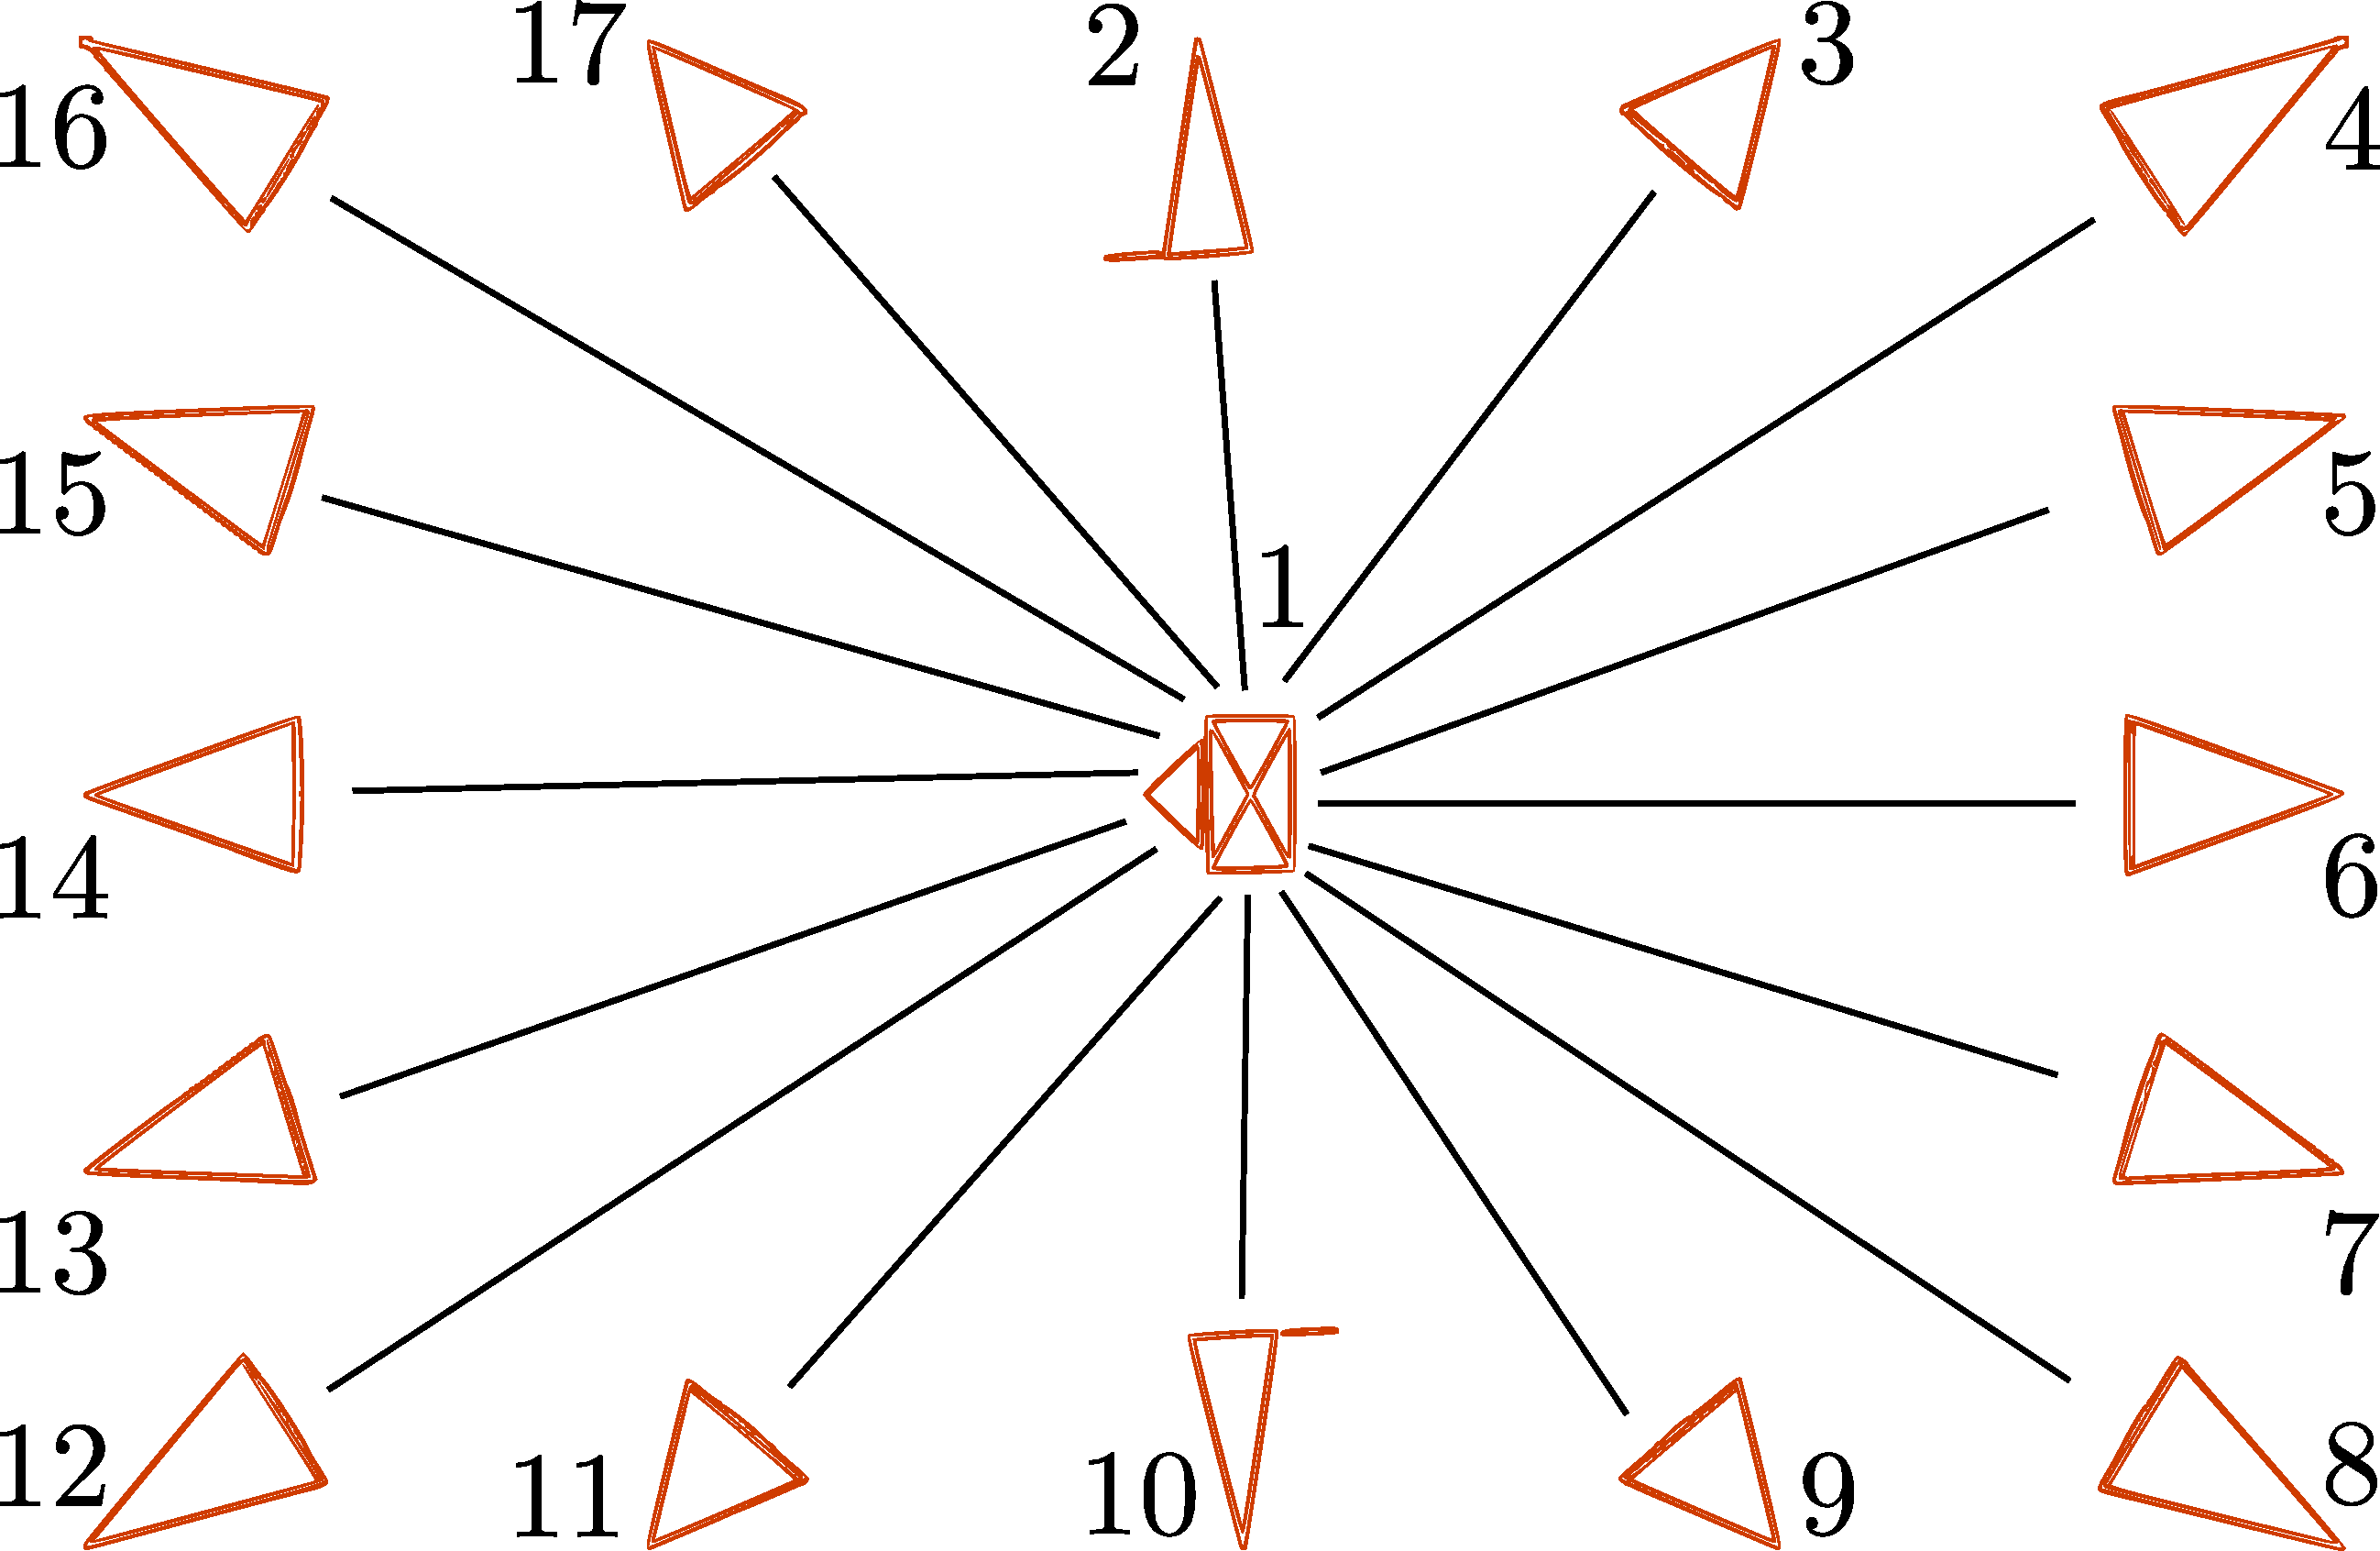
\includegraphics[scale=0.13]{img/Reconstruccion/enlazado_general}}\hspace{2cm}
    \subfloat[Cada cámara con su adyacente]{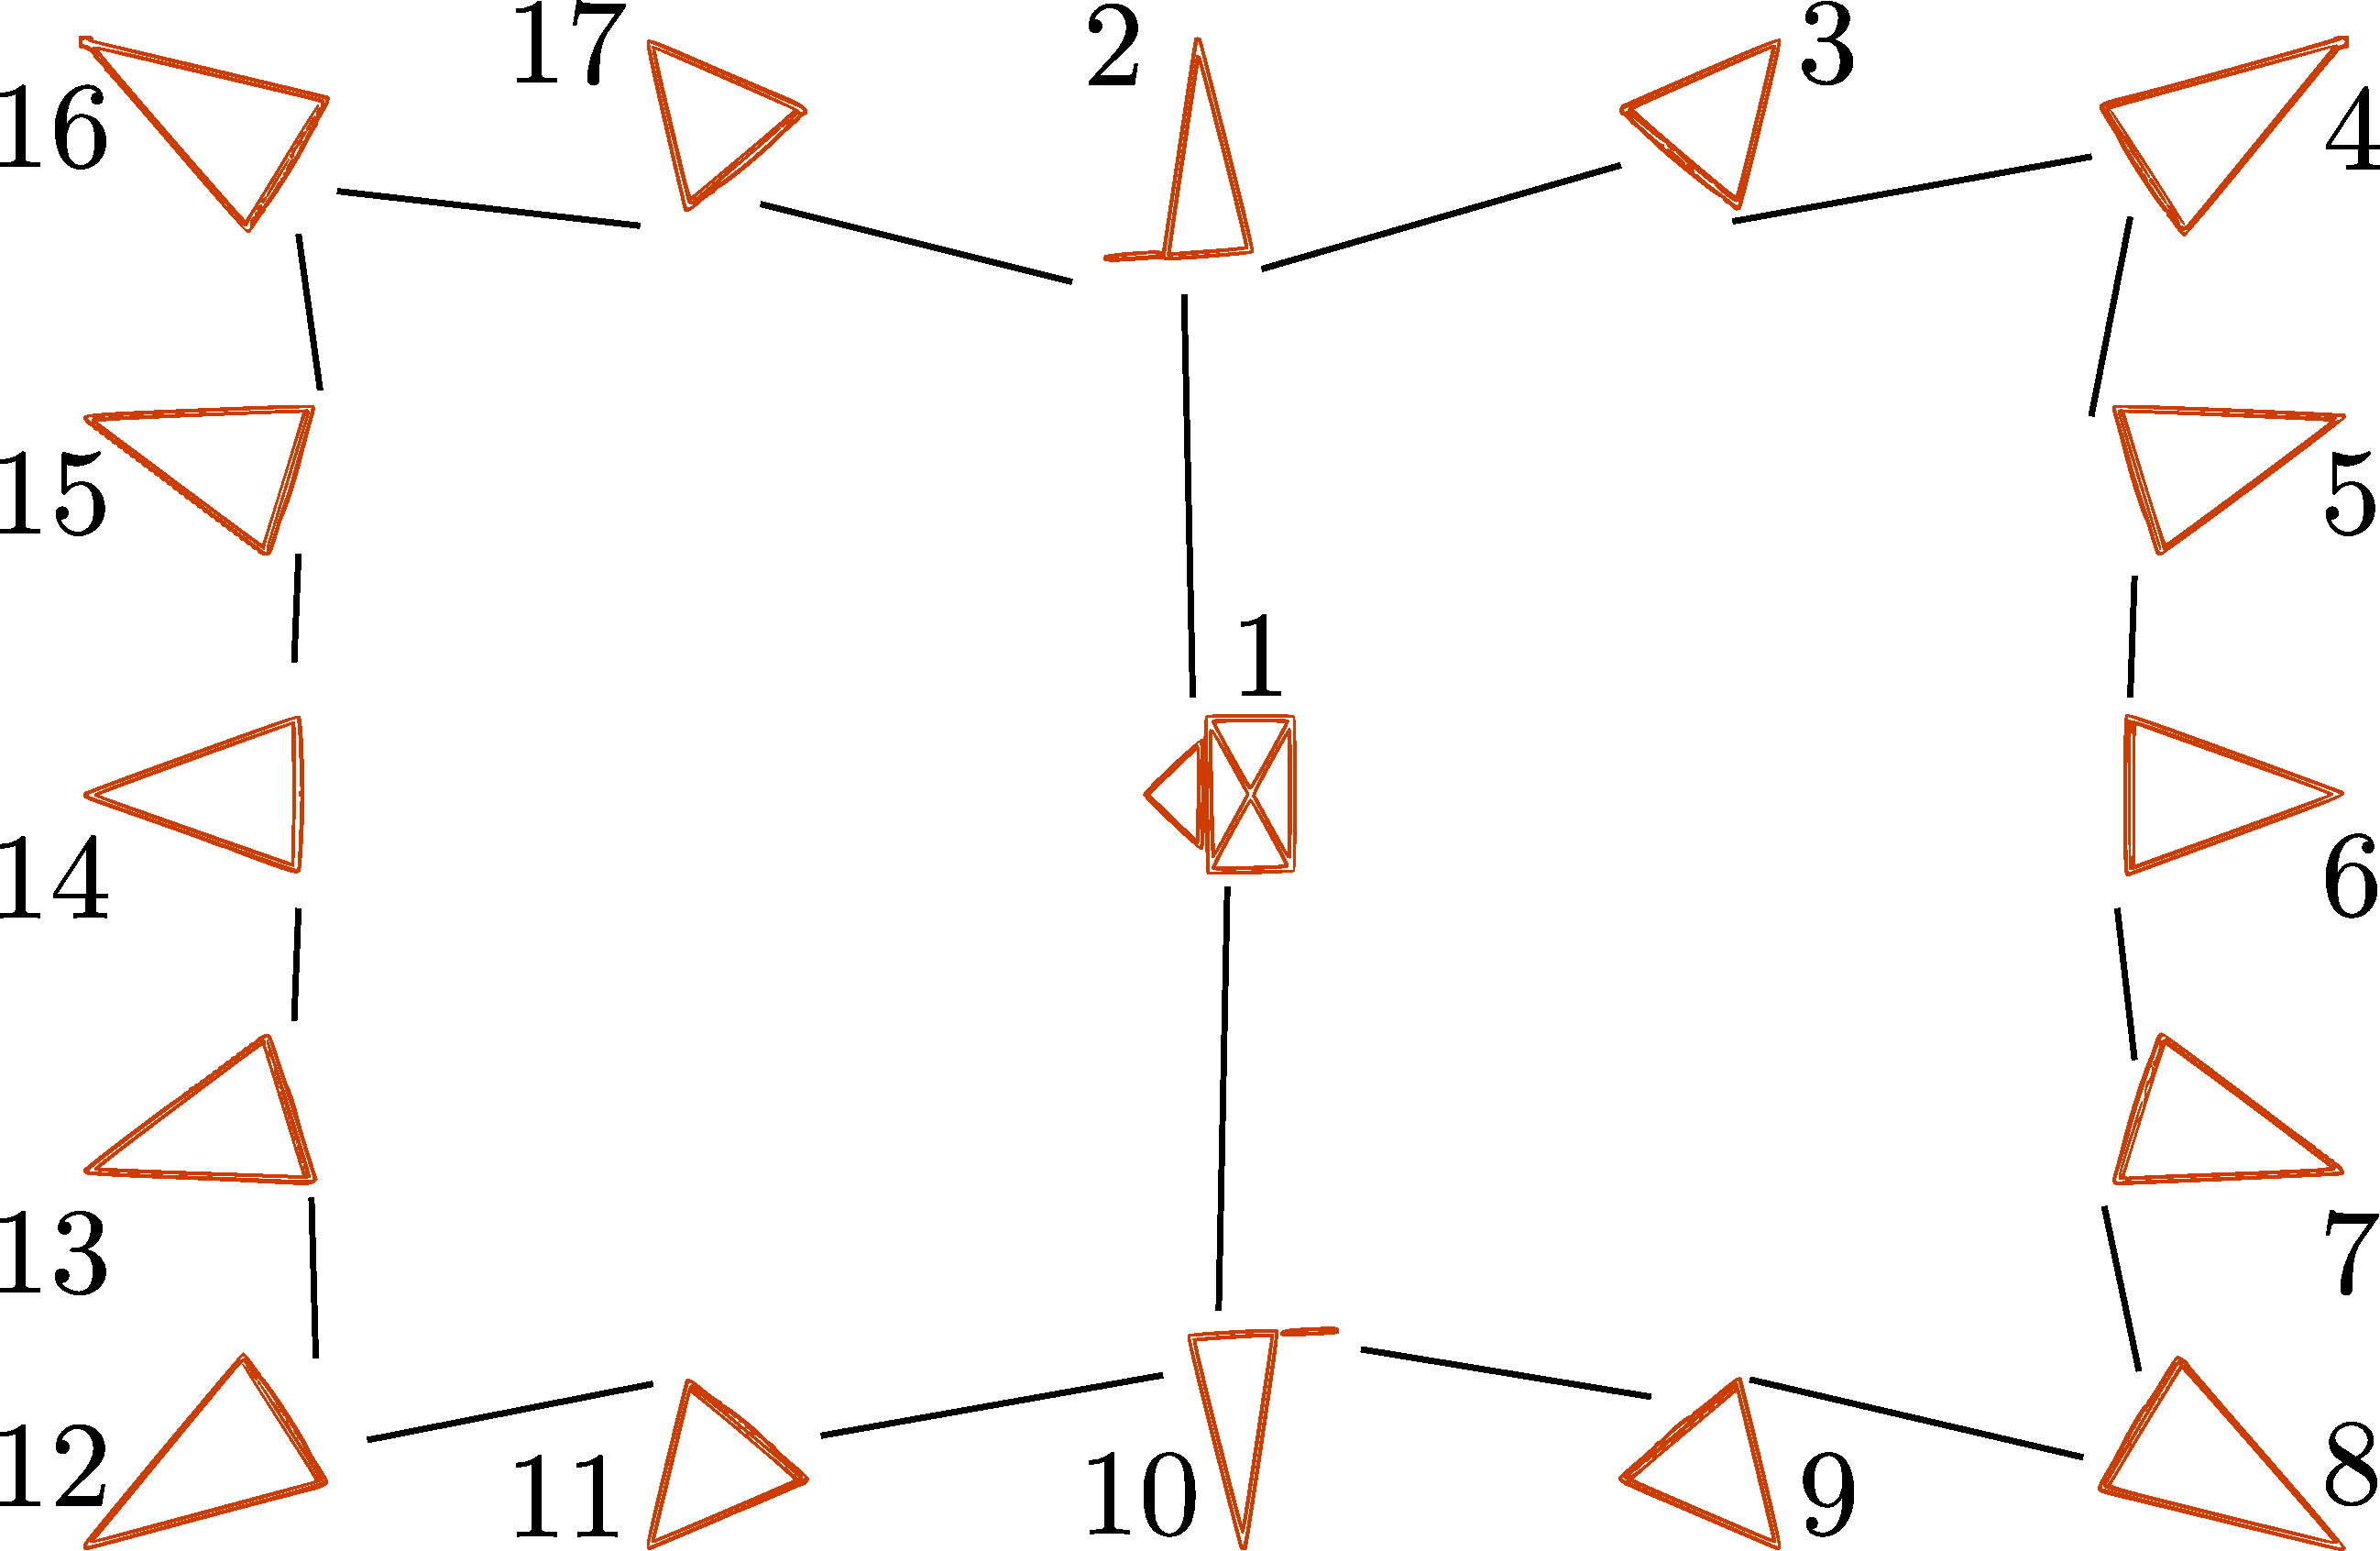
\includegraphics[scale=0.13]{img/Reconstruccion/enlazado_adyacente}\label{img_asociacion_consecutivas}}
   \caption{Métodos utilizados para generar pares de cámaras.}  
   \label{img_asociacion} 
 \end{figure} 





\subsection{Mejor asociación}\label{MejorAsociacion}

A partir de la lista con asociaciones entre puntos de dos vistas generada anteriormente, es necesario elegir aquella que posea mayor probabilidad de conformar la pareja de imágenes correspondiente a la proyección de un marcador 3D sobre dichas vistas.
%corresponder a la proyección en esas dos vistas de uno de los marcadores en el espacio.\\


Recordando que todas las asociaciones de puntos entre pares de cámaras se encuentran ordenadas por distancia, se toma aquella asociación que posea la menor distancia y contenga puntos válidos, descartando las restantes. Un punto se considera válido si en iteraciones anteriores no se a podido asociar a ningún punto 3D reconstruido (ver Sección \ref{actualizar_asociaciones}).
De esta forma cada punto de una cámara es asociado, si existen puntos válidos, con un punto en otra de las cámaras.


 Supongamos en la Figura \ref{fig: geometria_epipolar} que los puntos $x$ y $x'$ son la mejor asociación entre la cámara 1 y la cámara 2, y efectivamente son imágenes de un mismo punto 3D, idealmente los rayos de proyección se interceptarían en $X$, pero debido a incertidumbres en los procesos de calibración y segmentación la distancia entre dichos rayos no es nula, en el mejor de los casos solo es próxima a cero. 
Para evaluar cuál es entre los pares de puntos asociados disponibles el par que posee mayor posibilidad de corresponder a las proyecciones de un punto 3D, se proyectan todos los rayos de proyección y se toma aquella pareja de puntos que genere rayos de proyección con la menor distancia entre sí.


\subsection{Reconstrucción 3D y validación}\label{seccion_reconstruccion3D_validacion}


Luego de encontrar las mejores asociaciones entre dos cámaras se procede a reconstruirlas. Estas reconstrucciones deben ser validadas, para ello en principio se utiliza el  criterio propuesto por Herda \cite{herda}: se considera que una reconstrucción proveniente de dos cámaras es válida, si al proyectar sobre una tercera cámara existe al menos un punto de esta última que diste menos de un cierto valor umbral. Si efectivamente se encuentra al menos un punto, se asocia con los dos puntos que generaron la reconstrucción y se repite el proceso con el resto de las cámaras. Una vez finalizada la iteración, se retira a la pareja que genera la reconstrucción así como también a los puntos que lograron validarla, y se itera nuevamente repitiendo el proceso con la siguiente mejor pareja asociada entre dos cámaras. \\ 



\begin{figure}[ht!]
\centering
\hspace{-1cm}
\captionsetup{justification=centering,margin=1.0cm}
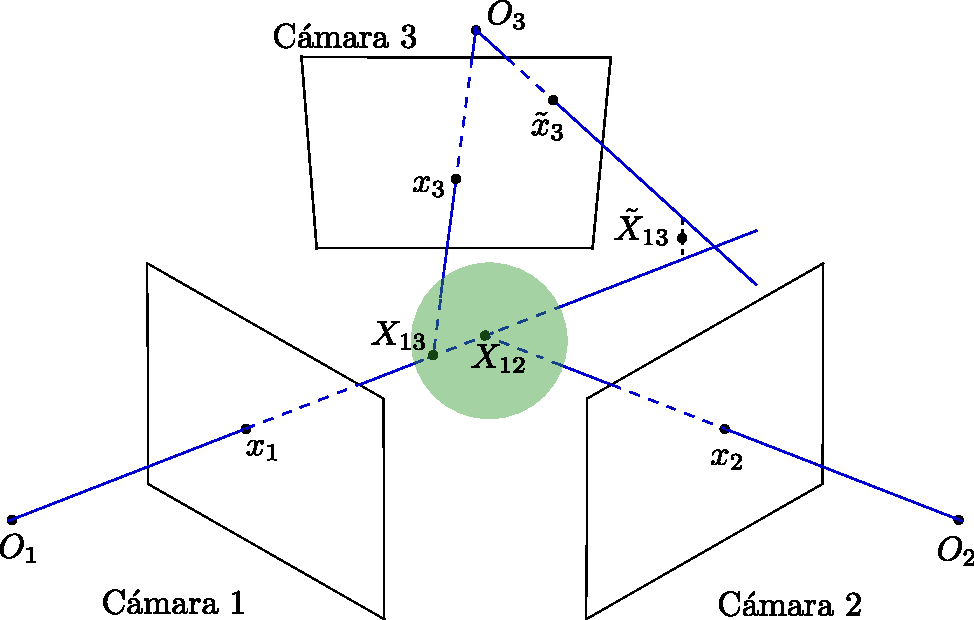
\includegraphics[scale=0.7]{img/Reconstruccion/validacion.pdf}
\caption{Reconstrucción entre cámaras 1, 2 y validación con cámara 3. El punto $x_3$ de la cámara 3 valida la reconstrucción, no así el punto $\tilde{x}_3$.}
\label{img_reconstruccion_validacion}
\end{figure}


El algoritmo desarrollado, si bien conceptualmente es similar, se implementa desde una óptica diferente computacionalmente más eficiente.
En lugar de llevar en cada iteración la información 3D a cada cámara, se procede a llevar la información de las cámaras una sola vez al espacio 3D y trabajar en cada iteración sobre el mismo. 


La información que contiene un punto en una retina se mapea en el espacio 3D sobre el rayo de proyección que contiene a dicho punto y al centro de la cámara correspondiente. Supongamos que se tienen los rayos de proyección en el espacio 3D de todos los puntos contenidos en las retinas y que $x_1$ es un punto en la cámara 1 de centro $O_1$ y $x_2$ es un punto en la cámara 2 de centro $O_2$ se encuentran asociados y reconstruyen al punto $X_{12}$ (ver Figura \ref{img_reconstruccion_validacion}). 


Idealmente $X_{12}$ se genera al interceptar los rayos de proyección de los puntos $x_1$ y $x_2$, pero debido a incertidumbres en la detección de marcadores o la calibración, comúnmente los rayos se van a cruzar. La reconstrucción, se estima como el punto del espacio de menor distancia a ambos rayos, por lo que
$X_{12}$ se encuentra en el punto medio del segmento perpendicular a ambos rayos.



El algoritmo implementado asume que un punto en una cámara, valida a $X_{12}$ si junto a $x_1$ reconstruye un punto 3D que se encuentra dentro de la esfera $B(X_{12}, \delta)$ de centro $X_{12}$ y radio $\delta$, donde $\delta$ es un cierto valor umbral. Notar que la elección anterior de $x_1$ sobre $x_2$ es indiferente para los propósitos de este proyecto. 


Si bien este criterio difiere del postulado original propuesto por Herda, en cierta manera se considera más robusto, pues en el postulado original basta con que dos puntos en una retina se encuentren lo suficientemente cerca para obtener una validación, pero esto no implica necesariamente que provengan de puntos 3D cercanos, sin embargo bajo el nuevo criterio si dos puntos 3D se encuentran cerca, entonces es válido afirmar que sus proyecciones sobre las distintas retinas también deben estarlo. Otra ventaja es que los umbrales bajo los cuales se considera que dos puntos están ``cerca'' difieren en cada una de las cámaras debido al distinto mapeo de distancias, sin embargo en el espacio 3D, manejar un único umbral resulta suficiente.       

\subsection{Actualizar asociaciones}\label{actualizar_asociaciones}

Del bloque anterior se tiene, un punto $X$ reconstruido y sus correspondientes proyecciones en cada una de las cámaras. Dichas proyecciones no deben ser consideradas nuevamente, por tanto estos puntos 2D que reconstruyen $X$, no se consideran como puntos válidos en las siguientes iteraciones.\\



Finalmente el proceso iterativo se detiene cuando no hay más marcadores para reconstruir, lo cual implica que se cumple alguna de las siguientes condiciones:\\
\begin{itemize}
\item el número de marcadores reconstruidos es igual al número de marcadores que tiene colocada la persona, o igual al número máximo de marcadores  reconstruidos que se haya indicado.

\item No existen puntos 2D válidos tal que pueda establecerse una asociación entre puntos de distintas vistas.
\end{itemize}




\section{Resultados de reconstrucción sobre secuencias sintéticas}

Se ha probado el algoritmo descrito anteriormente con secuencias capturadas en Blender. Para la configuración de 17 cámaras se han obtenido resultados aceptables,  con errores promedio en torno a los $0.5\,cm$. En la Sección \ref{seccion_performance}, se define la medida de error  y se evalúa el desempeño del algoritmo respecto a dicha medida. En dichas pruebas se observan resultados aceptables aún utilizando hasta 6 cámaras.

\begin{figure}[ht!]
\centering
\captionsetup{justification=centering,margin=0.2cm}
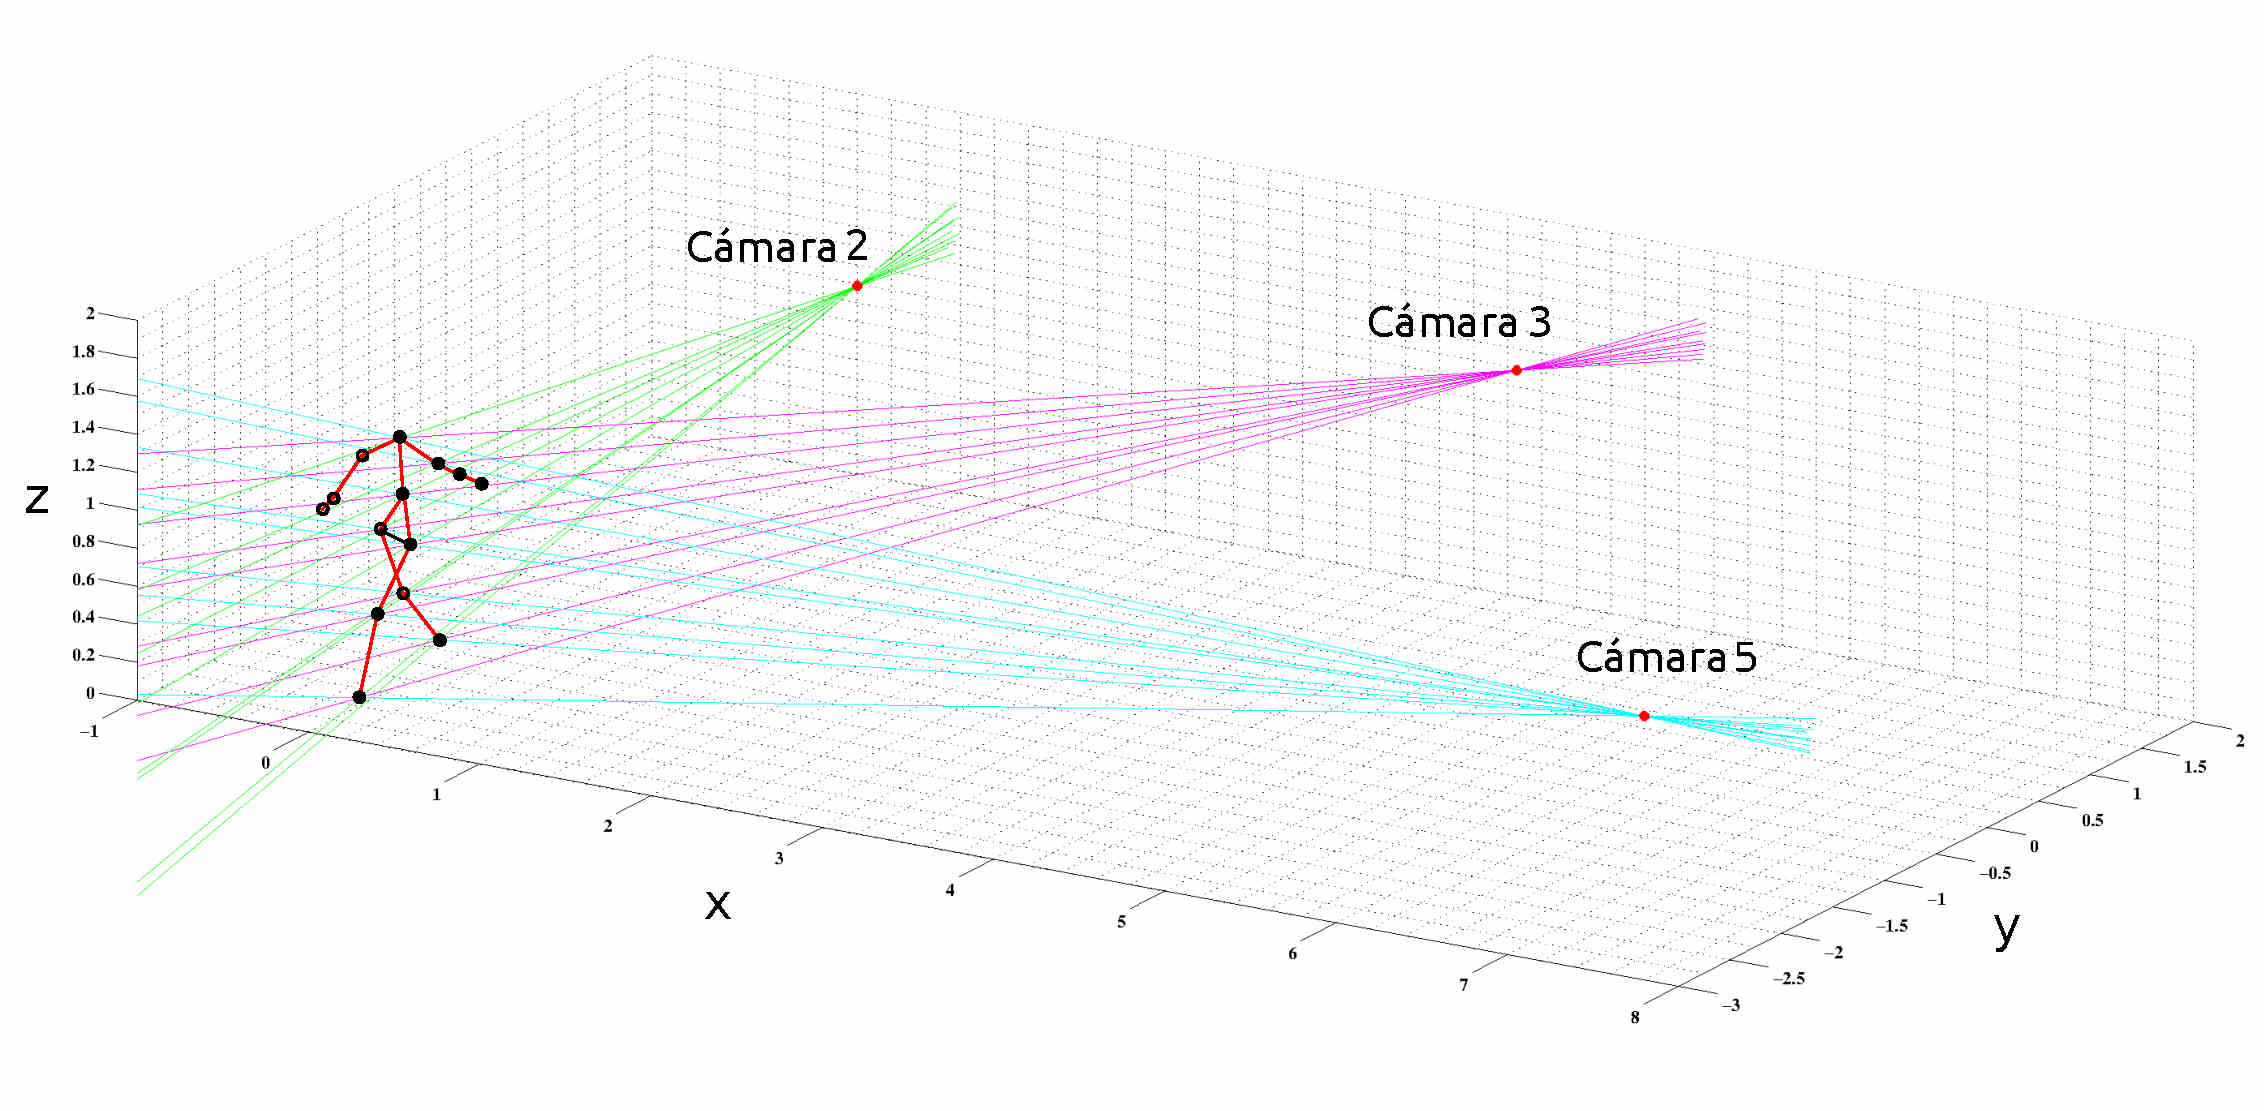
\includegraphics[scale=0.5]{img/Reconstruccion/Reconstruccion_3_camaras2.jpg}
\caption{Ejemplo del proceso de reconstrucción. Los marcadores totalmente negros son los que se pudieron reconstruir utilizando información de las cámaras 2, 3 y 5.}
\end{figure}


Como se menciona previamente se han realizado dos implementaciones distintas del bloque  \emph{Asociar puntos 2D} (Sección \ref{seccion_asociar2D_uno}), que se diferencian en el criterio para seleccionar los pares de cámaras:
\begin{itemize}
\item La primera implementación  considera las asociaciones de marcadores posibles entre pares de cámaras, evaluando cada una de las cámaras respecto a todas las restantes. 
\item La segunda implementación toma en cuenta  la configuración circular de las cámaras en el espacio y se evalúa cada cámara con la que se encuentra inmediatamente más cerca,  recorriendo las cámaras en algún sentido.
\end{itemize}
  

\begin{table}[ht!]
\hspace{-1cm}
\resizebox{15cm}{!} {
\begin{tabular}{cc|c|c|c|c|}
\cline{3-6}
                                                                              &                                                       & \multicolumn{2}{l|}{\textbf{Primera implementación}}                                                                                             & \multicolumn{2}{l|}{\textbf{Segunda implementación}}                                                                                            \\ \hline
\multicolumn{1}{|l|}{\begin{tabular}[c]{@{}l@{}}\textbf{Marker}\\ \textbf{Ground}\end{tabular}} & \begin{tabular}[c]{@{}l@{}}\textbf{Name}\\ \textbf{Ground}\end{tabular} & \begin{tabular}[c]{@{}l@{}}\textbf{Error} \\ \textbf{Promedio}\\ \textbf{(cm)}\end{tabular} & \begin{tabular}[c]{@{}l@{}}\textbf{Percentil}\\ \textbf{99\% (cm)}\end{tabular} & \begin{tabular}[c]{@{}l@{}}\textbf{Error}\\ \textbf{Promedio}\\ \textbf{(cm)}\end{tabular} & \begin{tabular}[c]{@{}l@{}}\textbf{Percentil}\\ \textbf{99\% (cm)}\end{tabular} \\ \hline
\multicolumn{1}{|l|}{1}                                                       & LeftUpLeg                                             & 0.4182                                                           & \textbf{3.7197}                                                        & 0.3671                                                          & 0.5158                                                        \\ \hline
\multicolumn{1}{|l|}{2}                                                       & LeftLeg                                               & 0.3586                                                           & 0.5449                                                        & 0.3670                                                          & 0.5411                                                        \\ \hline
\multicolumn{1}{|l|}{3}                                                       & LeftFoot                                              & 0.3862                                                           & 1.0379                                                        & 0.3720                                                          & 0.5580                                                        \\ \hline
\multicolumn{1}{|l|}{4}                                                       & RightUpLeg                                            & 0.3963                                                           & 1.7542                                                        & 0.3714                                                          & 0.5879                                                        \\ \hline
\multicolumn{1}{|l|}{5}                                                       & RightLeg                                              & 0.3830                                                           & 0.9840                                                        & 0.3780                                                          & 0.5860                                                        \\ \hline
\multicolumn{1}{|l|}{6}                                                       & RightFoot                                             & 0.4192                                                           & 1.5364                                                        & \textbf{0.4212}                                                          & \textbf{1.8483}                                                        \\ \hline
\multicolumn{1}{|l|}{7}                                                       & Spine                                                 & 0.4075                                                           & 0.9092                                                        & 0.4040                                                          & 0.6043                                                        \\ \hline
\multicolumn{1}{|l|}{8}                                                       & Head                                                  & 0.4130                                                           & 1.2853                                                        & 0.3867                                                          & 0.9063                                                        \\ \hline
\multicolumn{1}{|l|}{9}                                                       & LeftArm                                               & 0.3626                                                           & 0.6394                                                        & 0.3666                                                          & 0.7997                                                        \\ \hline
\multicolumn{1}{|l|}{10}                                                      & LeftForeArm                                           & \textbf{0.4774}                                                           & 2.8511                                                        & 0.3873                                                          & 0.9056                                                        \\ \hline
\multicolumn{1}{|l|}{11}                                                      & LeftHand                                              & 0.4217                                                           & 2.0700                                                        & 0.4007                                                          & 1.1722                                                        \\ \hline
\multicolumn{1}{|l|}{12}                                                      & RightArm                                              & 0.4756                                                           & 2.4363                                                        & 0.4025                                                          & 1.4771                                                        \\ \hline
\multicolumn{1}{|l|}{13}                                                      & RightForeArm                                          & 0.4590                                                           & 3.1711                                                        & 0.3844                                                          & 0.7810                                                        \\ \hline
\multicolumn{1}{|l|}{14}                                                      & RightHand                                             & 0.4545                                                           & 2.4782                                                        & 0.3816                                                          & 0.7728                                                        \\ \hline
\multicolumn{1}{l|}{}                                                         & \textbf{Secuencia }                                            & \textbf{0.38556 }                                                         & \textbf{1.7907    }                                                    & \textbf{0.35686}                                                         &\textbf{ 0.81266}                                                       \\ \cline{2-6} 
\end{tabular}
}
\caption{Performance de los algoritmos implementados en reconstrucción. }
\label{table_performance_reconstruccion}
\end{table}

En la Tabla \ref{table_performance_reconstruccion} se muestra una comparación de resultados. En la misma se observa que en la segunda  implementación el error promedio mejora ligeramente respecto a la primera implementación. Se observa también el error considerando el 99\% de los marcadores, donde la mejora de la segunda implementación es más significativa. Por esta razón se ha elegido la segunda de las implementaciones.


Una de las razones por las cuales puede suceder esto, es que en el primer algoritmo se realizan búsquedas de asociaciones entre marcadores detectados, en pares de cámaras donde la probabilidad de que un mismo marcador sea visto por ambas puede ser muy baja. El ejemplo más representativo es cuando se consideran cámaras que están  ubicadas en posiciones diametralmente opuestas. En este caso las asociaciones que se encuentren tienen mayores posibilidades de ser asociaciones incorrectas, influyendo negativamente sobre el desempeño global del algoritmo. 



\section{Resultados de reconstrucción sobre secuencias reales}

Para probar la reconstrucción con secuencias reales se realizó la calibración según lo explicado en la Sección \ref{seccion_calibracion_secuencias_reales}, por otra parte fue necesario robustecer el algoritmo de detección de marcadores como se explica en la Sección \ref{resultadosyanalisissegmentacion}. Las pruebas del algoritmo presentado anteriormente realizadas sobre esta secuencia no han dado resultados aceptables, en este caso la mayoría de los marcadores se reconstruyen erróneamente. 


Con el fin de encontrar donde falla el sistema se genera una secuencia sintética donde se utilizan tres cámaras para la captura. Dichas cámaras están ubicadas en posiciones relativas que simulan el caso real, de esta manera se procede a probar el sistema con dichas secuencias.  En este caso los resultados tampoco han sido aceptables. Tras varias pruebas se llega  a la conclusión de que la deficiencia del sistema es que el algoritmo de reconstrucción, no es lo suficientemente robusto para el caso en que se utilizan pocas cámaras.\\
% % % % % % % % % % % % % % % % % % % % % % % % % % % %
% % % % % %Poner UNA FIGURA DEL RESULTADO MOSTRANDO QUE TAN MALO ES.
% % % % % % % % % % % % % % % % % % % % % % % % % % % % %
Esta situación ha motivado el desarrollo de mejoras sobre este algoritmo. Los cambios se realizan sobre la implementación disponible del sistema, con el fin de lograr un desempeño aceptable sin modificar la estructura global del sistema.

\section{Mejoras del algoritmo de reconstrucción}


Se hicieron pruebas sobre la base sintética, nuevamente simulando la situación del caso real, con el fin de aislar los errores provenientes de la calibración y de la detección de marcadores.
El algoritmo que se implementa en este caso, con el fin de solventar dichos errores, tiene una estructura similar al considerado anteriormente (ver Figura \ref{fig: diagrama algoritmo}), aunque algunos bloques modifican su funcionamiento, fundamentalmente el primero (\emph{Asociar puntos 2D}).

\subsection{Asociar punto 2D}

En esta versión modificada, el resultado de \emph{Asociar puntos 2D} continúa siendo una lista ordenada de asociaciones entre puntos de distintas cámaras, pero el procedimiento para generar dicha lista es diferente. \\  

Para cada punto de una retina se genera una lista ordenada que asocia dicho punto con los puntos de las restantes retinas. El orden de la lista se establece según la distancia euclídea entre los rayos de proyección de los puntos a asociar.\\

De esta forma se obtiene una matriz de distancias entre rayos de proyección 3D. Cada columna de esta matriz es una combinación posible de dos rayos de proyección. Cada fila se compone de la siguiente manera:
\begin{itemize}
\item Número de cámara $\alpha$.
\item Índice del punto 2D cámara $\alpha$.
\item Número de cámara $\beta$.
\item Índice del punto 2D cámara $\beta$.
\item Distancia entre los rayos de proyección de los puntos considerados.
\end{itemize}



\begin{figure}[ht!]
\centering
\captionsetup{justification=centering,margin=2.8cm}
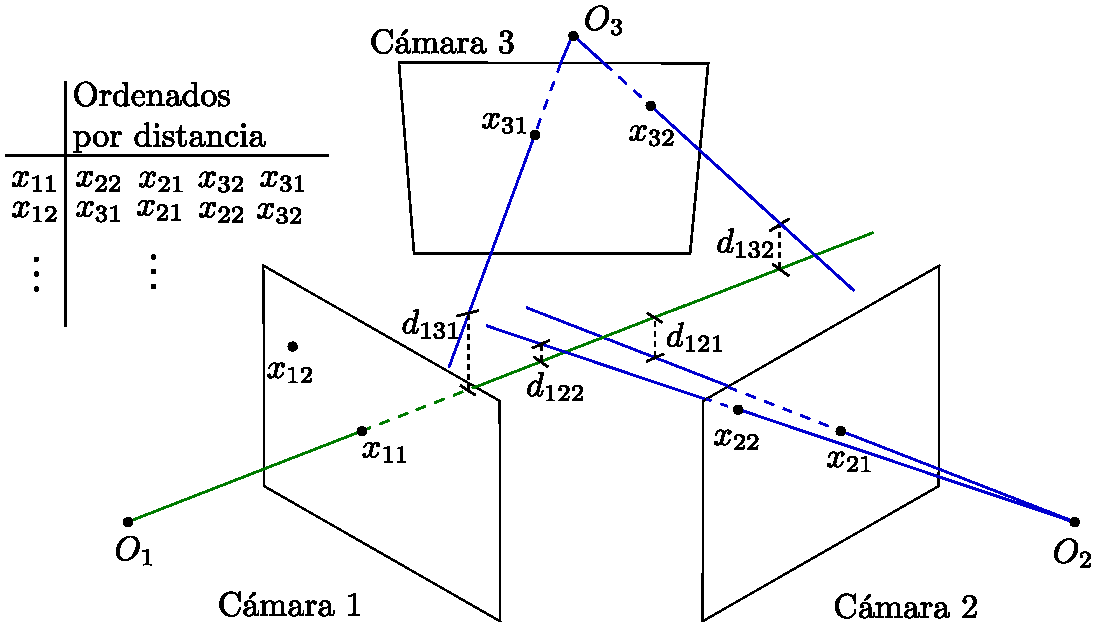
\includegraphics[scale=0.7]{img/Reconstruccion/Asociar_puntos_2}
\caption{Nueva asociación de puntos entre pares de cámaras.}
\end{figure}
 
\subsection{Mejor asociación}


Este bloque mantiene su funcionalidad, encontrar la pareja de puntos entre dos vistas, con mayor probabilidad de corresponder a la proyección de un punto 3D.
La diferencia fundamental con su implementación anterior es la gestión de las matrices de entrada, pues el ordenamiento por distancia de dichas matrices es diferente. 


En la primera implementación las distancias que producen el ordenamiento son generadas entre rectas epipolares y puntos, o sea distancias sobre un plano, mientras que en esta implementación las distancias son entre rayos en el espacio 3D.


Manteniendo el criterio original para implementar este bloque, el cual consiste en tomar la pareja de puntos que genere rayos de proyección con la menor distancia entre sí. 
La nueva entrada proporcionada por \emph{Asociar puntos 2D} simplifica la implementación a desarrollar.


Una vez que se tiene la matriz de distancias con todas las asociaciones de puntos entre los pares de cámaras considerados, este bloque simplemente toma de entre todas las asociaciones disponibles de puntos válidos, aquel par de puntos que posea menor distancia asociada.
Recordar que un punto se considera válido si en iteraciones anteriores no se ha podido asociar a ningún punto 3D reconstruido.

\subsection{Resto de los bloques}

Los bloques de \emph{Reconstrucción 3D y Validación}, y el de \emph{Actualizar Asociaciones} realizan el mismo funcionamiento y tiene igual implementación que los utilizados en el algoritmo anterior (ver Secciones \ref{seccion_reconstruccion3D_validacion} y \ref{actualizar_asociaciones}).

  Asimismo la condición que debe cumplirse para detener el proceso iterativo es la misma.

  
  
\section{Resultados del nuevo algoritmo}  


\begin{figure}[ht!]
   \centering 
    \subfloat[Vista derecha.]{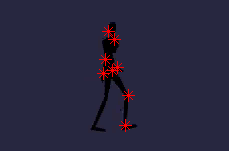
\includegraphics[scale=1.70]{img/Reconstruccion/50_derecha_sintetica.png}}\hspace{0.2cm}
    \subfloat[Vista  izquierda.]{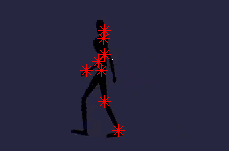
\includegraphics[scale=1.70]{img/Reconstruccion/50_izquierda_sintetica.png}}\hspace{2cm}
    \subfloat[Vista de atras.]{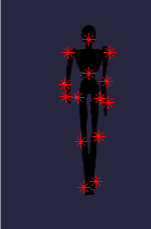
\includegraphics[scale=0.90]{img/Reconstruccion/50_atras_sintetica2.png}} \hspace{1.9cm}
    \subfloat[Resultado de la reconstrucción.]{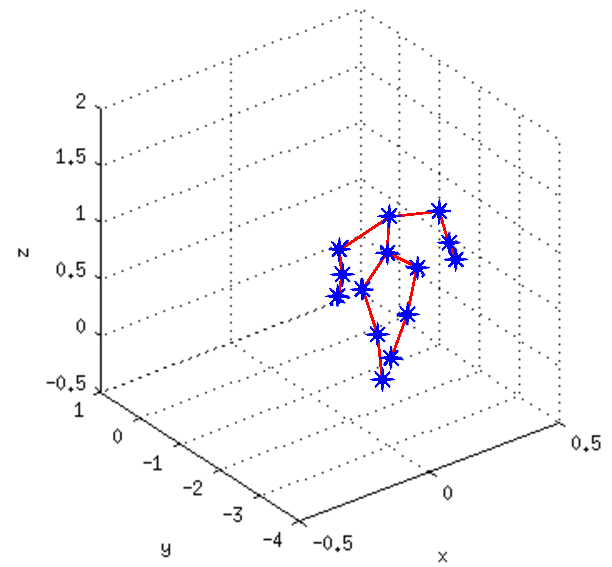
\includegraphics[scale=0.7]{img/Reconstruccion/50_matlab_sintetica.pdf}}    
   \caption{Reconstrucción de una secuencia sintética. Los asteriscos rojos indican los marcadores detectados.} 
   \label{img_reconstruccion_sintetica}    
\end{figure} 

 
Se prueba el nuevo algoritmo para una secuencia sintética de tres cámaras en las que se intenta simular el caso real. En este caso el sujeto cuenta con catorce marcadores. 
Los resultados muestran una mejora significativa respecto al algoritmo original
aunque no se llega a tener un desempeño ideal. 
De 20 cuadros relevados, en 11 de ellos se logra reconstruir de manera aceptable los 14 marcadores, en seis de los cuadros se tiene un marcador incorrectamente reconstruido y en los tres restantes se tiene dos marcadores incorrectamente reconstruidos.
En la Figura \ref{img_reconstruccion_sintetica} se muestra el resultado de la reconstrucción para un cuadro  determinado de la secuencia sintética.

\begin{figure}[ht!]
   \hspace{-1cm}
    \subfloat[Vista derecha.]{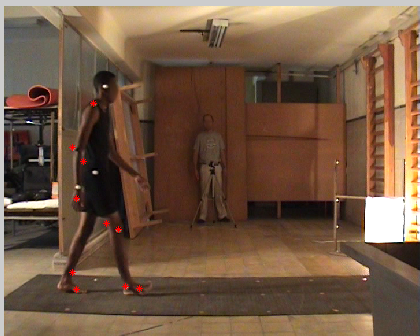
\includegraphics[scale=0.47]{img/Reconstruccion/22_derecha.png}}\hspace{0.3cm}
    \subfloat[Vista de atrás.]{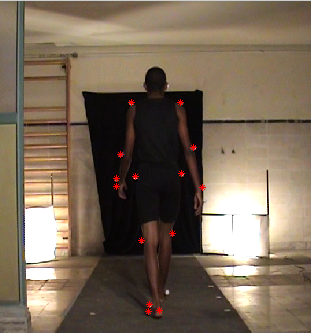
\includegraphics[scale=0.47]{img/Reconstruccion/22_atras.png}}\hspace{2cm}
    \subfloat[Vista izquierda.]{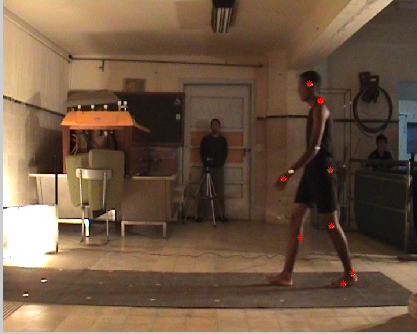
\includegraphics[scale=0.47]{img/Reconstruccion/22_izquierda.png}}\hspace{0.5cm}
    \subfloat[Resultado de la reconstrucción.]{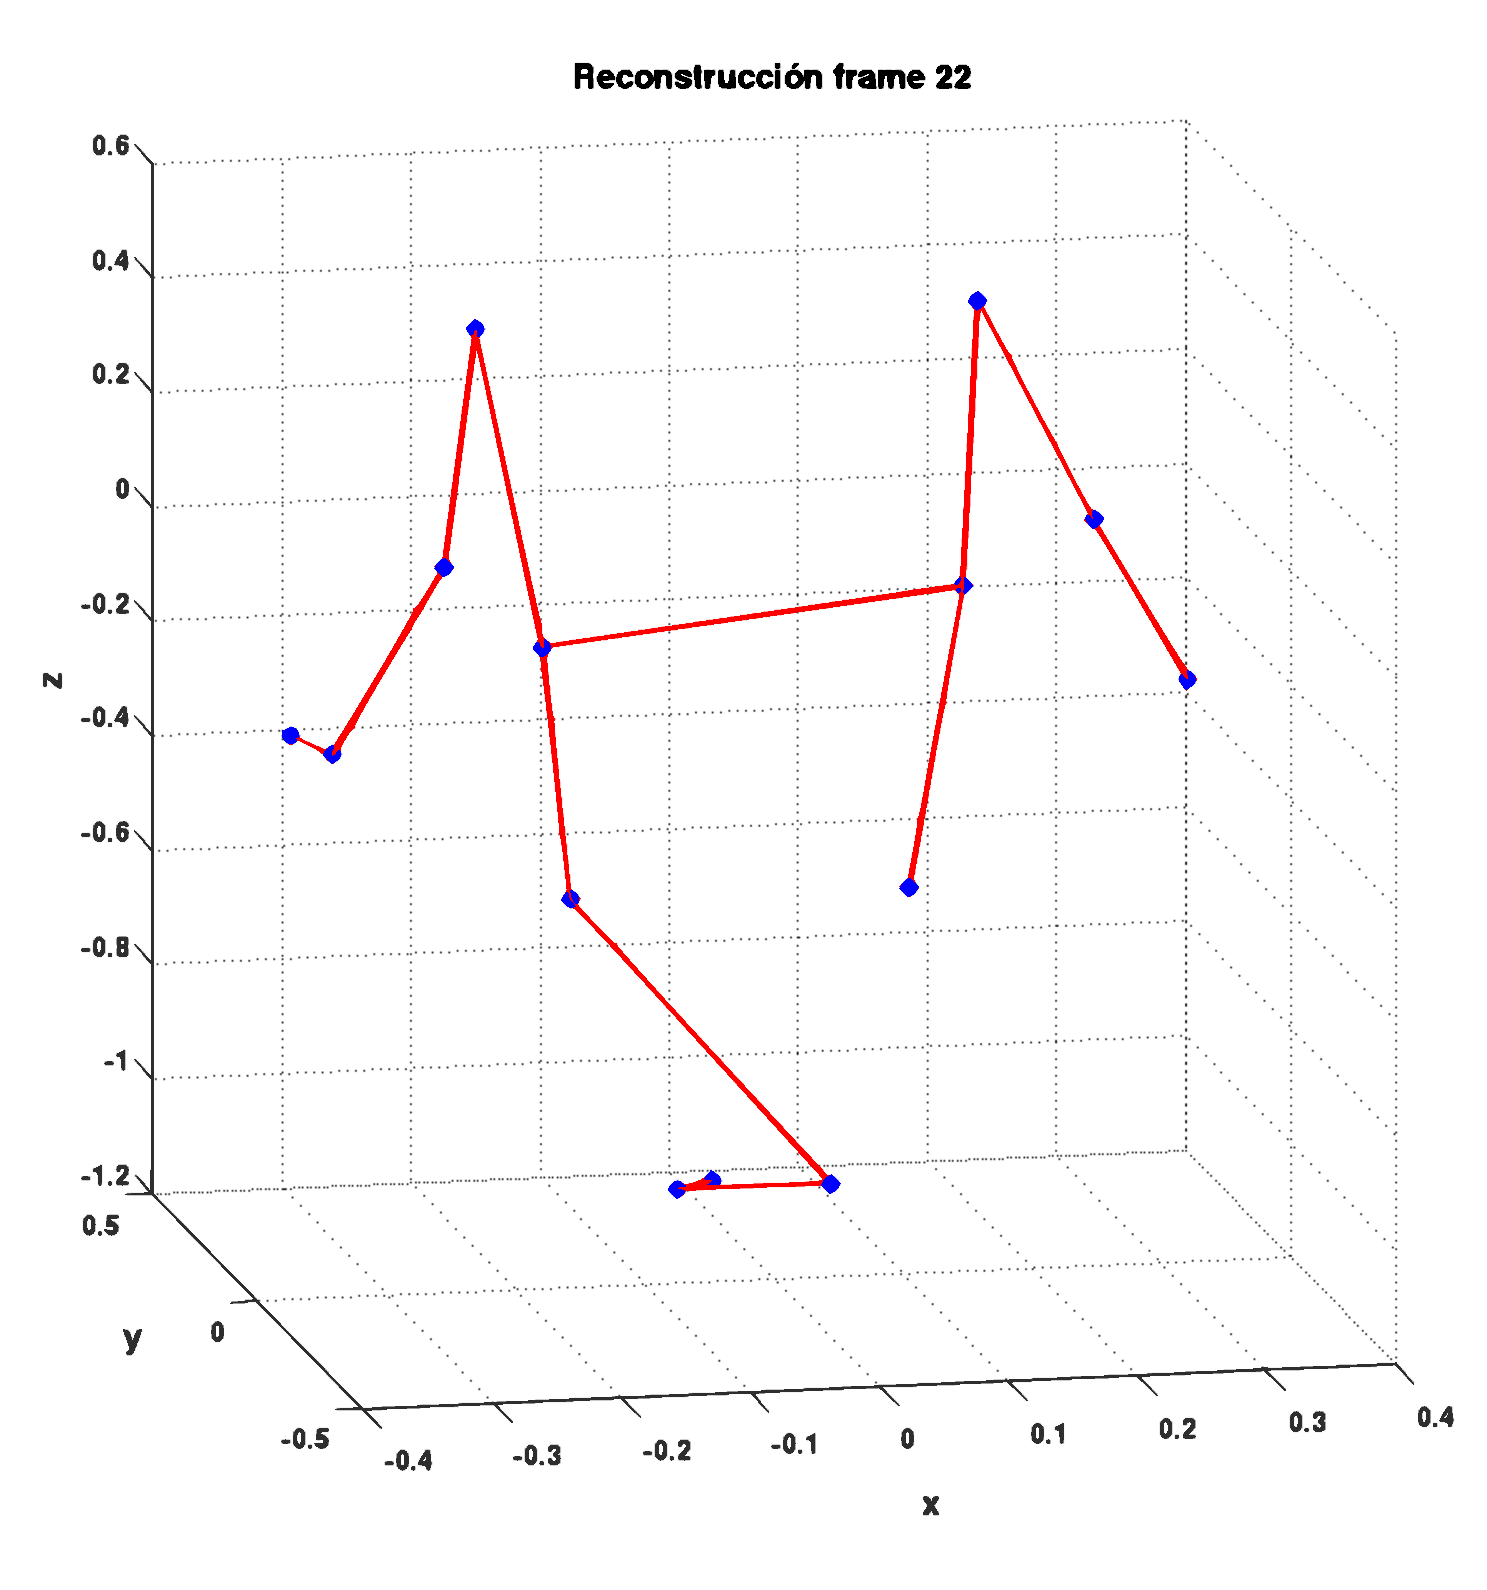
\includegraphics[scale=0.20]{img/Reconstruccion/frame22_esqueleto_armado.pdf}}
   \caption{Reconstrucción de una secuencia real. Los asteriscos rojos indican los marcadores detectados.} 
   \label{img_reconstruccion_real2}    
\end{figure} 

Por último el nuevo algoritmo fue probado con secuencias reales. Si bien se reconstruyen varios marcadores mejorando la performance que se tenía con el algoritmo de reconstrucción inicial, los resultados no son tan alentadores como los obtenidos para las secuencias sintéticas. En cierta manera es esperable dado que en este caso se adicionan errores provenientes de las etapas de detección de marcadores y de calibración. En la Figura \ref{img_reconstruccion_real2} se muestra el resultado obtenido para un cuadro de la secuencia real. 




\section{Conclusión} 

Tomando como punto de partida las ideas propuestas por Herda, referentes a la reconstrucción de puntos 3D a partir de múltiples imágenes de puntos sobre distintas cámaras,  se han diseñado e implementado dos variantes de algoritmo principal para la etapa de reconstrucción. Logrando probar dichos algoritmos sobre secuencias tanto sintéticas como reales se hace un análisis cualitativo de los resultados.\\


Inicialmente se genera un algoritmo con etapas bien definidas (ver Figura \ref{fig: diagrama algoritmo}), que obtiene resultados aceptables para secuencias sintéticas y configuraciones de más de seis cámaras. Como es de esperar la configuración espacial de las cámaras influye en el desempeño del algoritmo, por lo que la afirmación anterior es válida asumiendo una distribución de cámaras uniforme alrededor del espacio de captura.\\


Las pruebas realizadas sobre secuencias reales dejan presente el problema de desempeño que tiene el algoritmo cuando se utilizan pocas cámaras, produciendo resultados poco satisfactorios. 
En este caso, las secuencias reales obtenidas manejan tan solo tres cámaras y las condiciones de laboratorio no son las más favorables para efectuar un proceso de detección adecuado. Se ha visto que es necesario robustecer las etapas tanto de detección de marcadores  como de calibración, pues las incertidumbres producidas en dichas etapas tienen un efecto crítico sobre el desempeño de la reconstrucción. Con las secuencias reales disponibles, la falta de marcadores sobre las cámaras en la etapa de detección, es la mayor dificultad a enfrentar en el proceso de reconstrucción. \\



Con el fin de independizar la reconstrucción de los efectos de etapas anteriores, se introduce una secuencia sintética que simula el caso real, tanto en la calidad del movimiento como en el número y disposición de cámaras, donde los errores de calibración y detección de marcadores no son significativos.


Utilizando esta secuencia se implementa un nuevo algoritmo que mejora el desempeño en secuencias con pocas cámaras. Este nuevo algoritmo modifica parcialmente algunas etapas del algoritmo inicial, sobre todo la etapa de \emph{Asociar puntos 2D}, logrando obtener resultados significativamente mejores al tratar con pocas cámaras sobre el caso sintético.
Utilizando las secuencias reales, se obtiene mejoras cualitativas sobre el primer algoritmo, si bien el desempeño es inferior al caso sintético y la reconstrucción es apenas aceptable.  \\ 


De lo expuesto se desprenden fundamentalmente dos cosas:
\begin{itemize}
\item Las dificultades que ofrece el caso real, básicamente en la detección de marcadores, y cómo influye significativamente en la etapa de reconstrucción perjudicando el resultado final del sistema. Con lo cual se desprende que mejoras en la detección deberían tener un gran impacto en la reconstrucción.
\item El número de cámaras cambia significativamente el problema:
\vspace{-0.3cm}
\begin{itemize}
\item Por un lado se genera un algoritmo que gestiona de manera aceptable la redundancia de información que existe cuando se utiliza un número de cámaras superior al necesario para cubrir cierto espacio de captura (dadas las características de los movimientos tratados en este proyecto, básicamente de marcha rectilínea, el límite inferior para una reconstrucción aceptable son seis cámaras). Cabe recordar en este punto que los sistemas comerciales poseen generalmente como mínimo 8 cámaras e intentan trabajar con redundancia de información.
\item Por otro lado efectuando modificaciones al algoritmo anterior se genera un nuevo algoritmo, que permite trabajar con pocas cámaras pero no gestiona adecuadamente la redundancia de información.
\end{itemize}  
\end{itemize} 

El análisis en biomecánica exige restricciones sobre precisión espacial en los resultados de la reconstrucción, por lo que resulta necesario optimizar esta etapa. 

De lo visto en la bibliografía existente podría proponerse el uso de la información de esqueleto, teniendo presente que esto último, impone restricciones sobre las posiciones de los marcadores y particulariza los casos de uso del sistema. Si bien este tipo de análisis se menciona en el algoritmo propuesto por Herda, se decide en este trabajo generar un algoritmo en principio más general, con entradas y salidas bien determinadas y no se incorpora la información de esqueleto. \\
%VER CON GUILLERMO QUE QUISO PONER EN UNOS COMENTARIOS QUE ME PASO
 
 
 
%
%
%->Reconstrucción con base de datos sintética
%\\
%HABLAR Y MOSTRAR RESULTADOS DE La performance DE LA BASE DE DATOS AL UTILIZAR LAS DOS RAMIFICACIONES\\
%PROCEDIMIENTO DE ASOCIACIONES DEL TIPO TODO CONTRA TODO, Y ASOCIACIONES CON CÁMARAS CONSECUTIVAS.\\
%JUSTIFICAR POR LO TANTO QUE OFICIALMENTE NOS QUEDAMOS CON EL CASO DE ASOCIACIONES ENTRE CÁMARAS CONSECUTIVAS
%\\
%-----\\
%->CASO REAL
%\\
%\begin{itemize}
%\item introducción: SE PRUEBA SOBRE LO QUE SE TIENE DEL SISTEMA Y NO ANDA POR TAL Y TAL MOTIVO. pUES LA CALIBRACIÓN ES DIFERENTE NO SE OBTIENE RESULTADOS ACEPTABLES.
%
%\item EXPLICAR AJUSTE REALIZADOS, GENERACIÓN DE MINI-SISTEMA DONDE CORREN SECUENCIAS REALES.AQUÍ DEBE ESTAR EL NUEVO ALGORITMO DE RECONSTRUCCIÓN
%\begin{itemize}
%\item para todos los puntos contenidos en las retinas se trazan las correspondientes rectas de proyección 3D
%\item BLOQUE ASOCIACIÓN 3D: se asocian las rectas utilizando una métrica de distancia euclídea Las rectas de proyección que se encuentran a menor distancia entre si quedan asociadas.
%\item BLOQUE MEJOR ASOCIACIÓN: se elijen las n mejores asociaciones entre rectas 3D
%\item BLOQUE RECONSTRUCCIÓN: se reconstruyen los puntos 3D provenientes de las asociaciones anteriores 
%\end{itemize}
%
%\item EN DICHO MINI-SISTEMA SE SIMULA EN BLENDER EL CASO REAL Y SE INTENTA TENER ALGO MODERADAMENTE FUNCIONAL
%
%\item RESULTADOS -->ALGORITMO DE RECONSTRUCCIÓN OFICIAL(CASO ASOCIACIÓN ENTRE CÁMARAS CONSECUTIVAS) -->NO TUVO BUENOS RESULTADOS 
%\item CONSECUENCIA SE GENERA NUEVO ALGORITMO DE RECONSTRUCCIÓN QUE HACE TAL Y TAL COSA.
%\item CON ESTE NUEVO ALGORITMO SE OBTIENEN RESULTADOS ACEPTABLES SOBRE LAS SIMULACIONES DEL CASO REAL
%SE PRUEBA DICHO ALGORITMO SOBRE LOS DATOS REALES Y SE OBTIENEN RESULTADOS ACEPTABLES.
%\item JUSTIFICAR QUE LAS DIFERENCIAS SON DEBIDAS A CALIBRACIÓN (REAL VS SINTÉTICA) Y LA SEGMENTACIÓN (REAL VS SINTÉTICA).
%\item ¿CUALITATIVAMENTE SE PUEDE DECIR CUAL ES EL FACTOR QUE PERJUDICA EN MAYOR MEDIDA LOS RESULTADOS en la secuencia real RESPECTO AL CASO DE SIMULACIÓN SINTÉTICA?. Si la segmentación es lo que perjudica más, por tal y tal motivo.
%\end{itemize}
%
%\textbf{HABLAR DE LA INTEGRACIÓN DE ESTE NUEVO ALGORITMO EN EL SISTEMA COMPLETO.\\}
%\begin{itemize}
%\item para muchas cámaras (mas de 5 o 6, ver las pruebas de gonzalo) el sistema funciona razonablemente con la reconstrucción ``original''. Principalmente debido a que se cuenta con información redundante de los marcadores.
%\item para pocas cámaras se utiliza el nuevo algoritmo de reconstrucción, permite trabajar con la secuencia real disponible. con muchas cámaras el algoritmo puede ser computacionalmente complejo.
%\item explicar bien cual es la frontera entre uno y otro caso (5 o 6 cámaras?)
%\end{itemize}



\section{Seguimiento}

\subsection{Introducción}

La salida del bloque de reconstrucción, son los puntos 3D generados a partir de los múltiples vídeos de cada vista, presentados en el orden que fueron validados en cada frame (figura \ref{reconstr_00}). A su vez, los marcadores fueron reconstruidos tomando como entrada los puntos obtenidos en las imágenes de la segmentación, no teniendo estos información alguna sobre el cuerpo, mas que el orden en el que son generados al segmentar.

Son presentados sin orden definido para cada cuadro de la secuencia, y el objetivo del tracking o seguimiento, es identificarlos temporalmente, asignándoles una etiqueta constante a lo largo de la secuencia para cada marcador y obtener las trayectorias 3D.

\begin{figure}[hbt]
\begin{center}
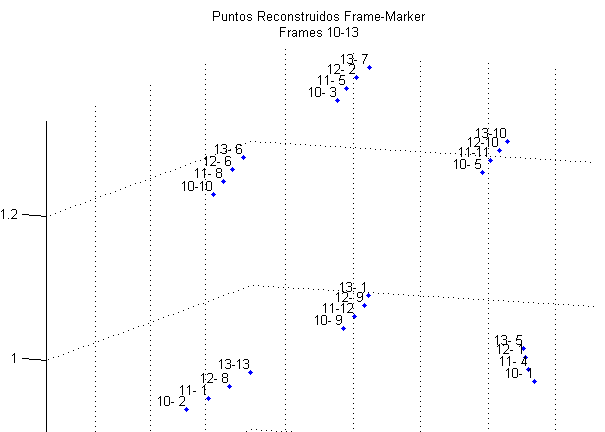
\includegraphics[scale=0.8]{img/Tracking/00_Salida_Reconstruccion.png}
\end{center}
\caption{Salida de Reconstrucción para 4 frames. La etiqueta para cada marcador es el frame y el indice en la reconstrucción}
\label{reconstr_00}
% Figura tomada de la reconstruccion 8_07_100_200
\end{figure}

\subsection{Estado del Arte}

El problema del seguimiento de marcadores espaciales a lo largo del tiempo es un tema de estudio habitual con distintos enfoques, entre ellos:

\begin{itemize}

\item Aplicación de restricciones al movimiento, teniendo información previa de los marcadores a estudiar, como se mueven, y como se relacionan entre ellos. 

\item Predictores Lineales o Estadísticos, teniendo información previa de una trayectoria para estimar el próximo elemento y confirmar o corregir la continuación de la secuencia.

\end{itemize}

Estos enfoques no son mutuamente excluyentes, pudiendo ser ambos complementarios para robustecer la generación de las trayectorias. Si se tiene acceso durante la adquisición de los datos, es posible relevar las distancias entre marcadores que se colocan en miembros que se mueven solidariamente  o dependen directamente uno del otro, por ejemplo al colocar marcadores en articulaciones de los brazos hay elementos sobre los huesos que siempre tendrán la misma distancia entre ellos (salvo una tolerancia, recordando que los marcadores no se encuentran en la articulación misma, sino sobre un lugar representativo sobre el cuerpo como se observa en el ajuste presentado en la figura \ref{skeleton_fitting_herda} , del ajuste planteado en el trabajo \cite{herda}. ). Con estas distancias relevadas y definidas las relaciones entre marcadores, es posible definir el esqueleto como una serie de restricciones que se mantienen a lo largo del tiempo (distancias entre marcadores solidarios) o varían de forma continua (angulo de huesos), donde la identificación es realizada inicialmente mediante un ajuste de los datos relevados en el mundo físico a los puntos obtenidos en la reconstrucción. 

\begin{figure}[hbt]
\begin{center}
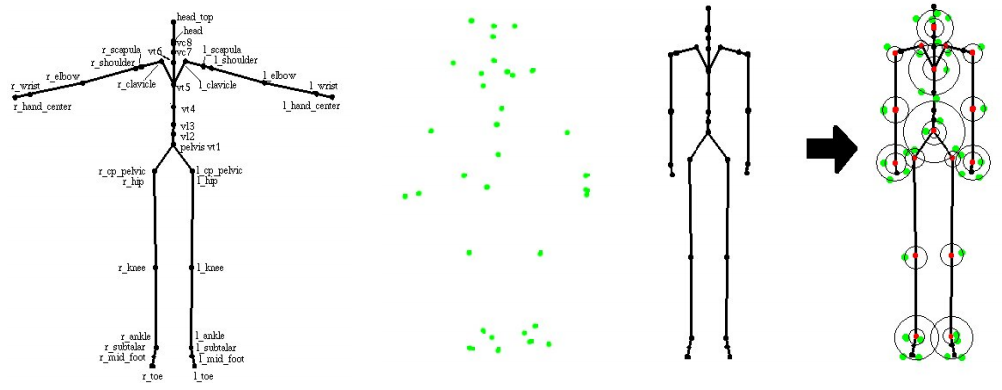
\includegraphics[scale=0.5]{img/Tracking/01_skeleton_fitting_Herda.png}
\end{center}
\caption{Inicializacion de esqueleto, y ajuste a los marcadores encontrados. Cada marcador representa una articulación y se ajusta en una esfera de cercanía centrada en la articulación del esqueleto}
\label{skeleton_fitting_herda}
\end{figure}.

Uno de los algoritmos mas simples \cite{survey_tracking}, es continuar una secuencia buscando el marcador mas cercano al ultimo punto conocido imponiendo la restricción que el traslado es mínimo ("greedy matching"), pero es susceptible a errores para casos muy simples, como se observa en el ejemplo de la figura \ref{greedy_matching} .

\begin{figure}[hbt]
\begin{center}
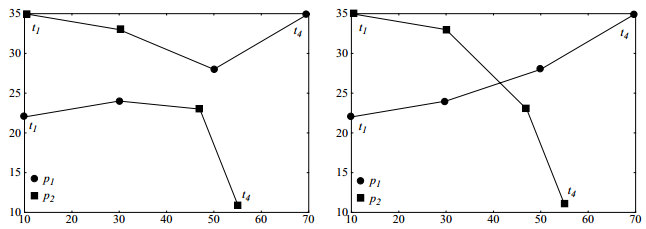
\includegraphics[scale=0.8]{img/Tracking/01_Greedy_Matching.png}
\end{center}
\caption{Dos marcadores moviéndose en cuatro frames, Izquierda corresponde al resultado de aplicar enlazado por elemento mas próximo \cite{survey_tracking} , Derecha al elegir el camino con variación mas suave}
\label{greedy_matching}
\end{figure}.

Para el caso de algoritmos de predicción, algunas soluciones implementadas para el tracking de marcadores son el filtro de Kalman \cite{kalman}, y sus variantes los cuales requieren inicializar y ajustar parámetros internos. Estos fueron implementados en las primeras instancias del estudio del problema, pero se decidió implementar otro procedimiento que sepa corregir los errores del método mas simple, no requerir estudio de parámetros internos para el filtrado, e ingrese alguna restricción a las trayectorias enlazadas.

El procedimiento elegido es el presentado por Lorna Herda\cite{herda} , y consiste en aplicar el tracking de partículas esbozado por Malik,Dracos,Papantoniou \cite{griegos} al seguimiento de marcadores. Este consiste en buscar el desplazamiento de un marcador desde el cuadro [f] al cuadro siguiente [f+1], sobre una ventana de cuatro cuadros.

La hipótesis principal de este algoritmo, es que el muestreo del movimiento capturado es suficiente para que el desplazamiento entre cuadros sea mínimo en distancia, y la idea para predecir y buscar el desplazamiento entre [f] y [f+1], es utilizar la información que se tiene de la secuencia entre [f-1] y [f], y utilizar una segunda proyección entre [f+1] y [f+2] para confirmar el enlace encontrado en el caso que exista mas de una posibilidad (figura \ref{herda_00}).

Para poder confirmar una trayectoria de 4 puntos, se debe cumplir que la misma presenta la menor variación de aceleración para la opción elegida entre todas las posibles, calculada como:

\begin{equation}
\begin{split}
\Delta{a}&= \left| \boldsymbol{\overrightarrow{a}}_{[f][f+1][f+2]}-\boldsymbol{\overrightarrow{a}}_{[f-1][f][f+1]} \right| \\
&= \left| \left(\boldsymbol{\overrightarrow{v}}_{[f+1][f+2]}-\boldsymbol{\overrightarrow{v}}_{[f][f+1]}\right).\Delta{t}-\left(\boldsymbol{\overrightarrow{v}}_{[f][f+1]}-\boldsymbol{\overrightarrow{v}}_{[f-1][f]}\right).\Delta{t} \right| \\
&= \left|\left( x_{[f+2]} - 3.x_{[f+1]} + 3.x_{[f]} - x_{[f-1]} \right).\Delta{t}^2\right|\\
\end{split}
\label{track_var_acc}
\end{equation}

, donde $x_{[f+1]}$ a su vez, es aquel punto de [f+1] que mejor se aproxima al desplazamiento en frames anteriores, minimizando la ecuación \ref{track_acc} 

\begin{equation}
\begin{split}
\boldsymbol{\overrightarrow{v}}_{[f][f+1]}& = \boldsymbol{\overrightarrow{v}}_{[f-1][f]} \\
x_{[f+1]}-x_{[f]}& = x_{[f]}-x_{[f-1]} \\
\end{split}
\label{track_acc}
\end{equation}

\begin{figure}[hbt]
\begin{center}
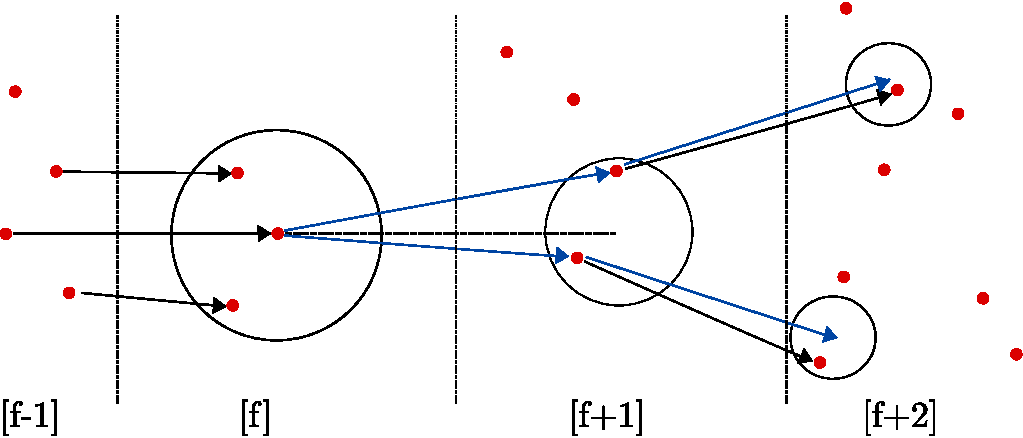
\includegraphics[scale=0.8]{img/Tracking/tracking-eps-converted-to.pdf}
\end{center}
\caption{Seguimiento en 4 frames, siendo [f] el frame actual que queremos seguir en [f+1]. La linea punteada es la traslación del movimiento previo, las lineas azules son las obtenidas buscando la mínima variación de aceleración para el punto elegido en [f+1]. De las dos posibles trayectorias, se elige aquella con menor variación de aceleración}
\label{herda_00}
\end{figure}

En su trabajo\cite{herda}, Lorna Herda propone que realizar el seguimiento sobre la reconstrucción 3D presenta menos continuidad en las trayectorias , con respecto al seguimiento realizado sobre el conjunto de segmentación sumada a la proyección de los puntos reconstruidos 3D en cada vista 2D. Sin embargo, en nuestras pruebas, nos pareció mas coherente trabajar con el seguimiento en los puntos reconstruidos en 3D, ya que en caso de trayectorias que se cruzan en una vista 2D, son fácilmente separadas en 3D debido a la geometría.

Adicionalmente, la reconstrucción fue implementada de forma distinta a la propuesta por Herda, si bien es posible obtener los puntos proyectados en cada vista, no cumplen el mismo rol. Sin implementar la re-proyección, en el tracking sobre una vista individual se pierden trayectorias cuando se pierden de vista como se observa en la figura \ref{tracking_2D_cam_07} .

\begin{figure}[hbt]
\begin{center}
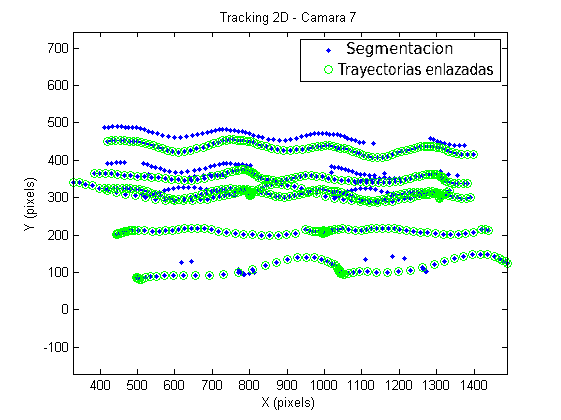
\includegraphics[scale=0.7]{img/Tracking/011_tracking_2D_camara_07.png}
\end{center}
\caption{Resultado de Aplicar el Seguimiento de marcadores a una vista 2D sin reproyección de puntos reconstruidos. Verde, las trayectorias que se enlazaron completamente, Azul los puntos segmentados en la vista 2D de la cámara 07 de la captura sintética}
\label{tracking_2D_cam_07}
\end{figure}

Finalmente, asumiendo que los puntos obtenidos directamente de las animaciones ,proyectados en cada cámara, son el mejor caso de puntos 2D, no presentaban grandes ventajas de trabajar el enlace en cada una de estas vistas 2D, sobre trabajar en 3D posteriormente a la reconstrucción, y no volver hacia atrás ya que la geometría entre vistas cumplió su cometido. Esto ultimo no se cumple para el caso que se evalúen medidas adicionales para robustecer la salida del tracking (por ejemplo, validación por visibilidad, un punto observado en la segmentación de una vista es descartado en caso de no ser físicamente posible ver ese punto entre el cuerpo y la cámara).

\subsection{Implementación}

Para un frame [f] y un marcador $m_{i}^{[f]}$, se desea encontrar en el frame [f+1] el marcador $m_{j}^{[f+1]}$ que continúe la trayectoria que se tiene hasta el momento, cumpliendo las ecuaciones de continuidad \ref{track_acc} y \ref{track_var_acc}. El elemento que traslada la información de un frame al siguiente y desde el anterior, es la matriz de enlaces, donde cada linea es un enlace, y cada enlace tiene los siguientes elementos:
\begin{equation}
\begin{bmatrix}
  m_{h}^{[f-1]} ,\quad m_{i}^{[f]} ,\quad m_{j}^{[f+1]} ,\quad m_{k}^{[f+2]} ,\quad \left|\boldsymbol{\overrightarrow{a}}_{[f-1][f][f+1]}\right| ,\quad \left|\boldsymbol{\overrightarrow{v}}_{[f][f+1]}\right|
\end{bmatrix}
\end{equation}

Para el ejemplo presentado en la figura \ref{reconstr_00} , en frame $f=11$ el marcador $m=8$ presenta el siguiente enlace hacia $(f+1)=12$, 

\begin{equation}
\begin{bmatrix}
  m_{3}^{[10]} ,\quad m_{8}^{[11]} ,\quad m_{3}^{[12]} ,\quad N/A ,\quad \left|\boldsymbol{\overrightarrow{a}}_{[10][11][12]}\right| ,\quad \left|\boldsymbol{\overrightarrow{v}}_{[1][12]}\right|
\end{bmatrix}
\end{equation}

, donde el indice en [13] no aplica debido a que no fue necesario para establecer en enlace entre [11][12].

Al final de cada iteración, la matriz de enlaces es consolidada para asignarle a cada nuevo marcador en [f+1] la etiqueta definida en el primer cuadro del enlazado, la cual puede ser inicializada como texto, si se le presenta la opción al usuario (en caso contrario, se utiliza el orden de los marcadores en el primer frame). Esta asignación será la que se utilice a lo largo de todo el seguimiento, por lo que todo marcador que no sea reconstruido en los primero frames, salvo de tomen medidas adicionales, no aparecerán en las trayectorias finales.

\subsubsection{Enlazado en régimen, inicial y final}

Dado un frame [f], se cargan todos los marcadores de los frames [f-1],[f],[f+1],[f+2], los cuales son puntos en coordenadas cartesianas $X,Y,Z$ (si el seguimiento desea hacerse para una vista 2D, se establece la tercer coordenada de todos los puntos en 1) en unidades correspondiente al plano donde se trabaja (pixeles para vistas 2D, metros para espacio 3D). Dentro de cada frame, los marcadores son identificados según su indice en la reconstrucción, y los enlaces de cada marcador [f-1][f], son cargados a partir de la matriz de enlace del frame anterior (la segunda y tercer columna de la matriz de enlace de [f-1], presenta los mismos datos que la primer y segunda columna de la matriz de enlace en [f], salvo el orden en que es presentada que es asociado al frame en curso).

Para el $i$-esimo marcador en [f], se relevan los indices que componen el enlace [f-1][f] para obtener el traslado previo, y aplicarlo para obtener el centro de búsqueda para el marcador en [f], cumpliendo la ecuación \ref{track_acc} .

\begin{equation}
\begin{split}
\boldsymbol{\overrightarrow{v}}_{[f][f+1]}^{i} = \boldsymbol{\overrightarrow{v}}_{[f-1][f]}^{i} \Rightarrow C_{[f+1]}^{i} &= x_{[f]}^{i} + \boldsymbol{\overrightarrow{v}}_{[f-1][f]}^{i}.\Delta{t} \\
&= 2.x_{[f]}^{i} -x_{[f-1]}^{i} 
\end{split}
\label{centro_busqueda_f1}
\end{equation}

La norma de este traslado es utilizada para evaluar los puntos cercanos al centro de búsqueda, donde pueden surgir tres casos:

\begin{itemize}
\item Se encuentra un solo punto dentro del radio de búsqueda , se agrega el indice del punto encontrado en [f+1] a los que se utilizaron de [f-1] y [f], calculando la aceleración y velocidad resultante para establecer el enlace. En este caso, el cuarto elemento de la linea de la matriz de enlace, no fue necesario 
\item Se encuentra mas de un punto, por lo cual se tiene que usar algún criterio para elegir entre todas la posibilidades encontradas. Para cada punto encontrado dentro del radio de búsqueda, se calcula un segundo centro de búsqueda para [f+2], esta vez minimizando la ecuación \ref{track_var_acc} :
\begin{equation}
\begin{split}
\boldsymbol{\overrightarrow{a}}_{[f][f+1][f+2]}=\boldsymbol{\overrightarrow{a}}_{[f-1][f][f+1]} \Rightarrow C_{[f+2]}^{i} &= x_{[f+1]}^{i} + \boldsymbol{\overrightarrow{v}}_{[f][f+1]}^{i}.\Delta{t} + \boldsymbol{\overrightarrow{a}}_{[f-1][f][f+1]}^{i}.\Delta{t}^2\\
&= 3.x_{[f+1]}^{i} - 3.x_{[f]}^{i} + x_{[f-1]}^{i}\end{split}
\label{centro_busqueda_f2}
\end{equation}
, siendo el radio de búsqueda en [f+2], la distancia [f][f+1]. Con los puntos encontrados en cada búsqueda de todas las posibilidades, se evalúa la variación de aceleración para los puntos [f-1][f][f+1][f+2], y elige la menor de todas, estableciendo el enlace de 4 puntos. Finalmente, se calcula la aceleración y velocidad del enlace [f-1][f][f+2], y se guardan los indices que permitieron la decisión, esta vez con cuatro elementos para indicar que se procedió con la segunda búsqueda.
\item No se encuentra ningún punto, tanto para la búsqueda en [f+1] como en [f+2]. En este caso, se presentan múltiples alternativas, en distintas etapas. La mas inmediata durante el enlazado frame a frame, es aumentar el radio de búsqueda (por ejemplo puede suceder con un punto acelerando y fuera del radio de búsqueda). Este aumento puede ser limitado, o indefinido hasta encontrar un punto aunque en una distancia mucho mayor a la esperada, por lo que deben ser validados posteriormente. Si el enlace pasa la validación dentro del frame, puede no pasar una validación posterior de trayectoria lo que se verá mas adelante
\end{itemize}

El enlazado final es similar a los presentado para régimen, pero en caso de múltiples marcadores candidatos en el frame final [f+1], no se puede extender el movimiento, por lo que se elige mediante menor aceleración en los últimos tres frames con una sola búsqueda desde [f] a [f+1], pero otra alternativa igualmente valida hubiera sido buscar sobre los últimos cuatro frames. Se eligió la primer opción debido a  ser un caso simplificado del enlazado en régimen ya implementada. 

Sin embargo, el enlazado inicial presenta una situación diferente, no se tiene información previa, y deben establecerse las bases para el inicio del enlazado. Para ello se cargan todos los marcadores en los primeros 3 frames, se calculan todas las posibles combinaciones de trayectorias entre elementos. En caso de existir combinaciones forzadas invalidas, las mismas presentan una aceleración resultante notoriamente mayor a la de enlaces, pero si corresponden a algún punto erróneo este se perderá naturalmente durante el enlazado,

Una vez enlazado el ultimo frame de las secuencia, se procede a limpiar aquellas trayectorias que perdieron marcadores en el camino estableciendo un umbral de perdida aceptables sobre el largo de las secuencias obtenidas. Adicionalmente, se descartan todos los puntos reconstruidos que no fueron asignados a ninguna trayectoria 


\subsubsection{Validación e Inventario de trayectorias}

Antes de consolidar la matriz de enlaces y proceder a que los marcadores en [f+1] hereden las etiquetas de las trayectorias a las que pertenecen, los enlaces deben ser validados en múltiples instancias:

\begin{itemize}
\item \textbf{Validación dentro del frame}: verificar que los indices de la matriz de enlaces en [f+1] son únicos, asociados a una sola trayectoria. Si dos o mas trayectorias se enlazaron a un mismo punto en [f+1], se comparará la aceleración con la que fueron enlazadas, validando aquella con menor aceleración, y descartando las otras. En este punto , existe la posibilidad de haber agregado todas las trayectorias involucradas en la decisión en vez de una sola trayectoria por marcador en [f+1], que mejor cumplía las condiciones para ese marcador. De haber elegido esta opción, el descartar una trayectoria que podría haber sido elegida por menor variación , daría paso a la siguiente mejor. Este caso sucedía mas en los casos que se aplico el seguimiento para trayectorias 2D, no tanto en 3D, por lo cual se terminó procediendo con solo una trayectoria por marcador, la cual en caso de ser invalida debe ser evaluada en la etapa de inventario de trayectorias  
\item \textbf{Validación en trayectoria}: pueden existir puntos que fueron reconstruidos con leves errores que deben detectarse, corregirse y estimar un reemplazo. Estos puntos son detectados como enlazados correctamente, pero con posición, velocidad, o aceleración que presenta una discontinuidad notoria, como puede observarse en el ejemplo de la figura \ref{discontinuidad_tracking} ,

\begin{figure}[H]
 \centering
  \subfloat[Trayectoria]{
   \label{track_m13}
    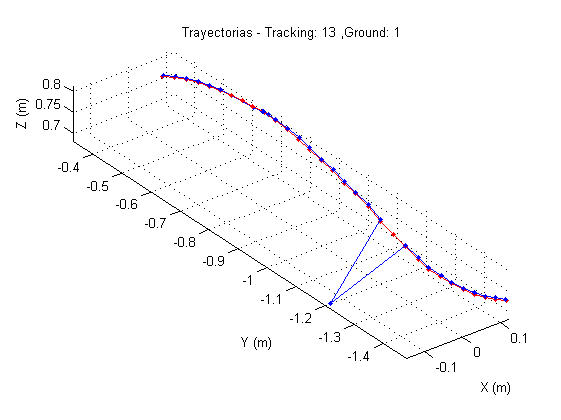
\includegraphics[width=0.5\textwidth]{img/Tracking/025_Salida_Tracking_Marker_13_8_07_100_200.png}}
  \subfloat[Velocidad,Aceleración,Variación Ac.]{
   \label{vel_acc_vacc_m13}
    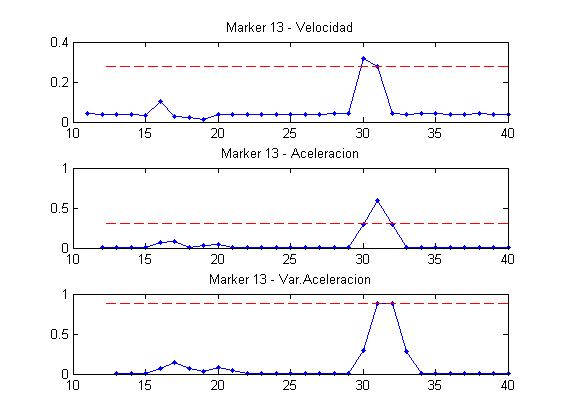
\includegraphics[width=0.5\textwidth]{img/Tracking/020_Salida_Tracking_Marker_13_8_07_100_200.png}}
 \caption{Ejemplo de discontinuidad en un marcador, por punto mal reconstruido. La figura \ref{track_m13} presenta en azul la trayectoria reconstruida, en rojo el ground truth}
 \label{discontinuidad_tracking}
\end{figure}

Se establece un umbral a partir del estudio de la distribución de la aceleración de cada marcador (figura \ref{distribucion_aceleracion} ) para encontrar la aceleración que presenta un salto abrupto, y detectar los frames donde se supera dicho umbral para corregir el marcador. El procedimiento para estimar los marcadores en estos casos, es el mismo que se verá al momento de inventario de trayectorias. 

Como opción mas global, se implementó una alternativa que en vez de calcular un umbral para cada trayectoria, establece un umbral global, el cual es útil para detectar aceleraciones notoriamente altas sin tener que estudiar cada trayectoria. Esta opción se implementó mediante una ejecución en dos instancias del seguimiento, una primera instancia sin limites globales de aceleración en en enlazado, y una segunda con un limite establecido a un porcentaje de la distribución de la aceleración, asumiendo un nivel a priori para perdidas (en nuestras pruebas, se estableció que filtrar al nivel que cumplan el 99\% de las aceleraciones de todos los marcadores enlazados arroja buenos resultados). Si durante la segunda instancia, un enlace global supera este umbral, se descarta y se procede con la recuperación de trayectoria.

\begin{figure}[H]
 \centering
  \subfloat[Función de distribución de la Aceleración]{
	\label{distribucion_aceleracion}
	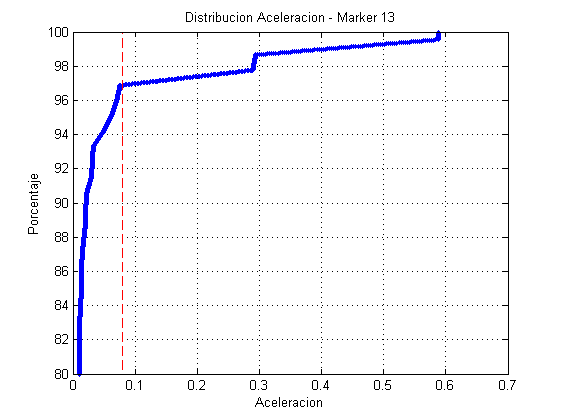
\includegraphics[width=0.5\textwidth]{img/Tracking/03_Distribucion_Aceleracion_Marker_13_8_07_100_200.png}}
  \subfloat[]{
   \label{track_m13_fix}
    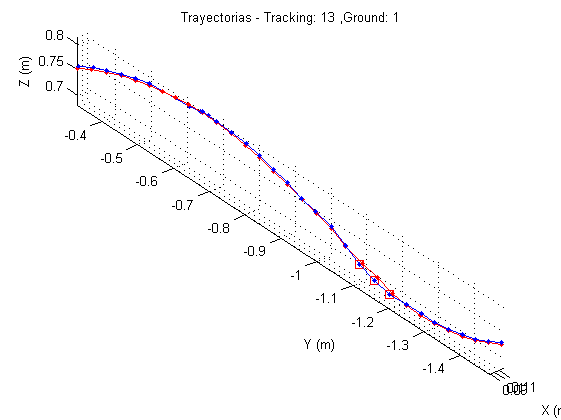
\includegraphics[width=0.5\textwidth]{img/Tracking/026_Salida_Tracking_Marker_13_8_07_100_200.png}}
 \caption{Ejemplo Resultado de Umbral y Corrección En Trayectoria}
% Figura tomada de la reconstruccion 8_07_100_200
\label{distro_acc_track_m13_fix}
\end{figure}
\item \textbf{Inventario de Trayectorias}: Durante el enlazado en un frame, se tienen marcadores en [f] que no lograron enlazarse en [f+1], pero cuya trayectoria podría estar enlazada hasta este frame.
Estos puntos deben ser identificados, mediante la comparación de la segunda columna de la matriz de enlaces [f][f+1] (actual) y la tercer columna de la matriz de enlaces [f-1][f] (anterior), ya que ambas tienen información de los marcadores en el mismo frame, pero enlazan hacia atrás y adelante.
Los elementos que se encuentren en la matriz [f-1][f] , pero no hayan sido enlazados en [f][f+1], son agregados a una lista que  contiene hasta que momento el frame mantenía el enlace (ultima vez que se tuvo información de la trayectoria a la cual pertenece), y que indice de marcador tenia en ese momento (pasar de indice en un frame, a trayectoria a la cual pertenece es trivial consultando las etiquetas de marcador que se van heredando de frame a frame).

Una vez actualizada la lista de las trayectorias perdidas en [f][f+1], se deben tratar de enlazar los puntos de [f+1] que no entraron en el enlazado regular, con las trayectorias perdidas hasta [f-1]. Todos los puntos que sobraron en el enlazado regular, son evaluados contra la lista de trayectorias perdidas, y se revisan dos condiciones:

\begin{enumerate}
  \item \textbf{Distancia con respecto a una estimación lineal}, prolongando el movimiento tomando el ultimo punto como inicio, y los últimos frames de la trayectoria conocida como desplazamiento. El desplazamiento es repetido tantas veces como tiempo perdido tiene el marcador: si una trayectoria estaba definida hasta [f-1] y se buscan enlaces con elementos de [f+1], el desplazamiento es repetido dos veces, como puede observarse en el ejemplo de la figure \ref{track_m8_recover}. 
 
\begin{figure}[H]
 \centering
  \subfloat[Salida de Código durante perdida y recuperación de trayectoria]{
	\label{track_m8_recover_code}
	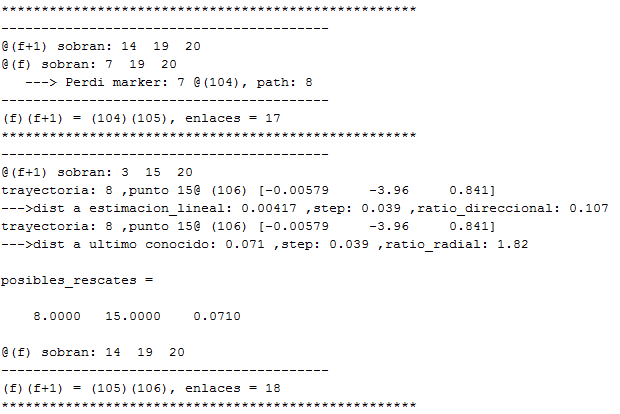
\includegraphics[scale=0.7]{img/Tracking/035_Salida_Codigo_Recuperacion.png}}\hspace{3 mm}
	
  \subfloat[Trayectoria]{
   \label{track_m8_recover}
\includegraphics[scale=0.7]{img/Tracking/030_Inventario_trayectoria_direccional.png}}
\caption{Trayectoria perdida en frame 104, con posible candidato de recuperación en frame 106 por cercanía con la estimación por desplazamiento}
% Figura tomada de la reconstruccion 8_07_100_200
\label{inventario_trayectoria_direccional}
\end{figure} 
  
  \item \textbf{Distancia radial con respecto al ultimo punto conocido}. En algunos casos, la perdida del enlazado puede suceder cuando la trayectoria está en reposo (por ejemplo, un pie apoyado antes de volver a despegarse del suelo), o en transición (en el medio de una curva), por lo cual la estimación lineal anterior es invalida. Para ello, es útil relevar la distancia entre el ultimo punto conocido de una trayectoria trunca, y los puntos que no se enlazaron en [f+1]. Esta distancia, en caso de una posible recuperación, deberá ser proporcional al ultimo traslado conocido, por la diferencia temporal de frames entre el ultimo punto, y el posible candidato.
 
El procedimiento de validación indica que marcadores son inválidos, tanto usando el umbral global, como el individual, pero esta validación puede truncar una trayectoria durante el enlazado que luego debe ser estimada en caso de recuperación, o debe ser filtrado para el caso de post-procesamiento. Se debe establecer un procedimiento para tratar de recuperar estos marcadores, tratando de cumplir con las restricciones impuestas.
 
  
\end{enumerate} 

\end{itemize}

\subsubsection{Estimación de Marcadores Perdidos Durante Enlazado}

Si se encuentra algún punto que cumpla alguna de las condiciones de recuperación de trayectorias, es considerado para continuar la trayectoria, y deben estimarse los puntos intermedios para completar la trayectoria.

Esta estimación es realizada mediante mínimos cuadrados, donde las condiciones iniciales dependen de cuantos puntos de la trayectoria se tenían hasta el momento, la condición final es el punto encontrado en [f+1], las incógnitas son los puntos intermedios que se quieren encontrar, y las múltiples ecuaciones a cumplir son las planteadas en (\ref{track_var_acc}) y (\ref{track_acc}).

Sea $X_{[f+1]}$ un punto candidato por las condiciones anteriores, y el ultimo punto conocido en [f-1] de un trayectoria que pretende continuar, verifica [f-1]$\geq$3, entonces las ecuaciones que el punto a estimar $\boldsymbol{\tilde{X}_{[f]}}$ deberá cumplir, (observar que las ecuaciones de variación de aceleración son combinación lineal de las ecuaciones de aceleración)

\begin{equation}
\left\{
\begin{matrix}
X_{[f-3]} &-3.X_{[f-2]} &+3.X_{[f-1]} &-\boldsymbol{\tilde{X}_{[f]}} & &=0 \\
 &X_{[f-2]} &-3.X_{[f-1]} &+3.\boldsymbol{\boldsymbol{\tilde{X}_{[f]}}} &-X_{[f+1]} &=0 \\
 &X_{[f-2]} &-2.X_{[f-1]} &+\boldsymbol{\boldsymbol{\tilde{X}_{[f]}}} & &=0 \\
 & &X_{[f-1]} &-2.\boldsymbol{\boldsymbol{\tilde{X}_{[f]}}} &+X_{[f+1]} &=0 \\
\end{matrix}
\right.
\label{ecuaciones_estimacion_01}
\end{equation}

, escribiendo de forma matricial, separando los datos en incógnitas y condiciones,

\begin{equation}
\begin{split}
&\begin{pmatrix}
1 &-3 &3 &-1&0\\
0 &1 &-3 &3 &-1\\
0 &1 &-2 &1 &0\\
0 &0 &1 &-2 &1\\
\end{pmatrix}
\begin{pmatrix}
X_{[f-3]}\\
X_{[f-2]}\\
X_{[f-1]}\\
\boldsymbol{\tilde{X}_{[f]}}\\
X_{[f+1]}\\
\end{pmatrix} =
\begin{pmatrix}
1 &-3 &3\\
0 &1 &-3\\
0 &1 &-2\\
0 &0 &1\\
\end{pmatrix}
\begin{pmatrix}
X_{[f-3]}\\
X_{[f-2]}\\
X_{[f-1]}\\
\end{pmatrix}+
\begin{pmatrix}
-1\\
3\\
1\\
-2\\
\end{pmatrix}
\boldsymbol{\tilde{X}_{[f]}}+
\begin{pmatrix}
0\\
-1\\
0\\
1\\
\end{pmatrix}
X_{[f+1]} = 
\begin{pmatrix}
0\\
0\\
0\\
0\\
\end{pmatrix} \\
&\Rightarrow
\underbrace{
\begin{pmatrix}
-1\\
3\\
1\\
-2\\
\end{pmatrix}
}_{A_{[f]}}\boldsymbol{\tilde{X}_{[f]}} = \underbrace{- \begin{pmatrix}
1 &-3 &3\\
0 &1 &-3\\
0 &1 &-2\\
0 &0 &1\\
\end{pmatrix}
\begin{pmatrix}
X_{[f-3]}\\
X_{[f-2]}\\
X_{[f-1]}\\
\end{pmatrix} - \begin{pmatrix}
0\\
-1\\
0\\
1\\
\end{pmatrix}
X_{[f+1]}}_{B_{[f]}} \\
&\Rightarrow \boldsymbol{\tilde{X}_{[f]}} = \left( A_{[f]}^{t}.A_{[f]}\right)^{-1}.A_{[f]}^{t}.B_{[f]}
\end{split}
\label{matrices_estimacion_01}
\end{equation}

El procedimiento presentado para aproximación de puntos es análogo para el caso de tener $n$ frames a estimar entre el ultimo momento $f_{i}$ de una trayectoria, y su posible continuación en $f_{j}$, con $n+1=f_{j}-f_{i}$. Si $f_{i} \geq 3$ , se plantearán $n+1$ ecuaciones para variación de aceleración, y $n+1$ ecuaciones para variación de velocidad (aceleración), las cuales se resuelven de la misma forma. 

\begin{equation}
\left\{
\begin{matrix}
X_{[f_{i}-2]} &-3.X_{[f_{i}-1]} &+3.X_{[f_{i}]} &-\boldsymbol{\tilde{X}_{[f_{i}+1]}} & & & &=0 \\
& X_{[f_{i}-1]} &-3.X_{[f_{i}]} &+3.\boldsymbol{\tilde{X}_{[f_{i}+1]}} &-\boldsymbol{\tilde{X}_{[f_{i}+2]}} & & &=0 \\
& & X_{[f_{i}]} &-3.\boldsymbol{\tilde{X}_{[f_{i}+1]}} &+3.\boldsymbol{\tilde{X}_{[f_{i}+2]}} &-\boldsymbol{\tilde{X}_{[f_{i}+3]}}& &=0 \\
& & & \ddots & \ddots & \ddots & \ddots & \\
& & & \boldsymbol{\tilde{X}_{[f_{j}-3]}} &-3.\boldsymbol{\tilde{X}_{[f_{i}-j]}} &+3.\boldsymbol{\tilde{X}_{[f_{j}-1]}} &-X_{[f_{j}]} &=0 \\
\end{matrix}
\right.
\label{ecuaciones_estimacion_n}
\end{equation}

En caso que la información previa a la perdida es menor, con $f_{i} \geq 2$, se plantea una ecuación menos, aquella que plantea la variación de aceleración de aceleración con el primer elemento incógnita que es la única que precisaría tres elementos previos, las otras ecuaciones no tienen problemas para plantearse.

Esta metodología de estimación de puntos intermedios es retomada para la validación en trayectoria, donde las incógnitas pasan a ser lo puntos que deben ser regularizados debido a presentar aceleración excesiva y discontinua para el marcador ( como fue establecido al principio de esta sección).




\subsection{Resultados y Análisis}

El objetivo del bloque de seguimiento es identificar los puntos reconstruidos, presentarlos como trayectorias, y corregirlos si es necesario. Por esta razón, es esperable que para una misma secuencia, los resultados sean similares a la reconstrucción, siendo las únicas leves diferencias las correcciones realizadas sobre trayectorias particulares, y la posibilidad de medir el error por marcador individual ya que a esta altura del algoritmo ya están identificados las distintas trayectorias. Los siguientes resultados fueron probados sobre una captura sintética de 113 frames, 14 marcadores, a lo largo de 17 cámaras.

\begin{figure}[hbt]
\begin{center}
\includegraphics[width=\linewidth]{img/Tracking/040_Salida_Tracking_Esqueleto_Trayectoria.png}
\end{center}
\caption{Tracking sobre captura sintética, 113 frames, 17 cámaras, 14 marcadores}
\label{Tracking_Esqueleto_Trayectoria}
\end{figure}

El filtrado y validación por trayectorias, permite reducir el error máximo y mejorar el promedio de trayectorias especificas (marcador 8 en figura), pero al aplicar global mente puede perjudicar a aquellas trayectorias que tengan naturalmente discontinuidades en aceleración debido a variaciones abruptas de movimiento (Tabla \ref{tablaerrortrack}). Para todos los marcadores, el error promedio se encuentra por debajo de 0.5 cm para la reconstrucción sobre vídeos sintéticos de la secuencia CMU-8-07-100-200 con 17 cámaras, y con el filtrado por aceleración individual de marcadores. En otras capturas, los comportamientos son similares con promedios inferiores a 0.5 cm, y errores máximos por debajo de 3 cm, para el caso de reconstrucción con 17 cámaras.Mas adelante se estudiará el impacto de cambiar los conjunto de cámaras en marcadores   

\begin{table}[h]
\begin{tabular}{|c|c|c|c|c|c|c|}
\hline
\begin{tabular}[c]{@{}c@{}}Marker\\ Track\end{tabular} & \begin{tabular}[c]{@{}c@{}}Marker\\ Ground\end{tabular} & \begin{tabular}[c]{@{}c@{}}Name\\ Ground\end{tabular}       & \begin{tabular}[c]{@{}c@{}}Error\\ Promedio(cm)\end{tabular} & \begin{tabular}[c]{@{}c@{}}Percentil\\ 99\%(cm)\end{tabular} & \begin{tabular}[c]{@{}c@{}}Error Promedio\\ (filtrado)(cm)\end{tabular} & \begin{tabular}[c]{@{}c@{}}Percentil 99\%\\ (filtrado)(cm)\end{tabular} \\ \hline
12       & 1         & LeftUpLeg          & 0,3671                                                       & 0,5158                                                       & 0,4042                                                                  & 2,0371                                                                  \\ \hline
3        & 2         & LeftLeg            & 0,367                                                        & 0,5411                                                       & 0,5456                                                                  & 2,7576                                                                  \\ \hline
2        & 3         & LeftFoot           & 0,372                                                        & 0,558                                                        & 0,377                                                                   & 0,7558                                                                  \\ \hline
6        & 4         & RightUpLeg         & 0,3714                                                       & 0,5879                                                       & 0,4033                                                                  & 1,6849                                                                  \\ \hline
4        & 5         & RightLeg           & 0,378                                                        & 0,586                                                        & 0,446                                                                   & 2,1396                                                                  \\ \hline
14       & 6         & RightFoot          & 0,4212                                                       & 1,8483                                                       & 0,4447                                                                  & 1,8483                                                                  \\ \hline
9        & 7         & Spine              & 0,404                                                        & 0,6043                                                       & 0,4103                                                                  & 0,7652                                                                  \\ \hline
7        & 8         & Head               & 0,3867                                                       & 0,9063                                                       & 0,3923                                                                  & 1,2422                                                                  \\ \hline
8        & 9         & LeftArm            & 0,3666                                                       & 0,7997                                                       & 0,3617                                                                  & 0,594                                                                   \\ \hline
13       & 10        & LeftForeArm        & 0,3873                                                       & 0,9056                                                       & 0,3961                                                                  & 1,1897                                                                  \\ \hline
10       & 11        & LeftHand           & 0,4007                                                       & 1,1722                                                       & 0,4128                                                                  & 1,4842                                                                  \\ \hline
1        & 12        & RightArm           & 0,4025                                                       & 1,4771                                                       & 0,3866                                                                  & 0,944                                                                   \\ \hline
11       & 13        & RightForeArm       & 0,3844                                                       & 0,781                                                        & 0,3945                                                                  & 0,8591                                                                  \\ \hline
5        & 14        & RightHand          & 0,3816                                                       & 0,7728                                                       & 0,411                                                                   & 1,1087                                                                  \\ \hline
         &           & \textbf{Secuencia} & \textbf{0,35686}                                             & \textbf{0,81266}                                             & \textbf{0,38305}                                                        & \textbf{1,6747}                                                         \\ \hline
\end{tabular}
\caption{Medida de error de tracking en captura de la base de datos sintética.}
\label{tablaerrortrack}
\end{table}

\begin{figure}[H]
 \centering
  \subfloat[Trayectoria sin Corregir Por Aceleración]{
	\label{Salida_Tracking_Original}
	\includegraphics[scale=0.5]{img/Tracking/036_Salida_Tracking_Original.png}}
  \subfloat[Trayectoria Corregida Por Aceleración]{
   \label{Salida_Tracking_Filtrado}
\includegraphics[scale=0.5]{img/Tracking/037_Salida_Tracking_Filtrado.png}}
\hspace{3 mm}
  \subfloat[Error de Marcador, sin Corregir]{
	\label{Salida_Tracking_Original}
	\includegraphics[scale=0.5]{img/Tracking/038_Salida_Tracking_Error_Marker_8_original.png}}
  \subfloat[Error de Marcador, Corregido]{
   \label{Salida_Tracking_Filtrado}
\includegraphics[scale=0.5]{img/Tracking/039_Salida_Tracking_Error_Marker_8_filtrado.png}}
\caption{Corrección por variación de aceleración, medidas de error antes y después de corregir}
% Figura tomada de la reconstruccion 8_07_100_200
\label{Tracking_Original_Filtrado_Errores}
\end{figure}


Al tener las etiquetas constantes para las trayectorias, es posible visualizar la relación entre marcadores, quedando pendientes medidas adicionales para robustecer el sistema, como imponer restricciones al movimiento entre marcadores en un mismo miembro, por imponer no solo continuidad en aceleración de marcadores sino ángulos de articulaciones y huesos. Esta continuidad debe tener cierta tolerancia debido a que los marcadores son representativos de articulaciones, y no se mueven completamente solidarios por lo que existen leves variaciones en las distancias entre marcadores, como se observa en la figura \ref{distancia_angulo_marcadores_piernas}, correspondiente a los marcadores asociados a la pierna en la captura 8\_03\_100\_100. En este caso se observa la continuidad y periodicidad de el angulo entre marcadores así como la constancia de la distancia, salvo momentos ocasionales, asociados a momentos específicos de la captura (cuando el pie rompe el reposo por ejemplo, antes de dar otro paso) ,sin ser mayor a los pocos centímetros en momentos puntuales y recuperables en régimen.

\begin{figure}[H]
 \centering
  \subfloat[Trayectorias de marcadores de pierna]{\includegraphics[scale=0.45]{img/Tracking/050_Salida_Tracking_13_14_10.png} %\label{trayectorias_marcadores_piernas}
   }	
  \subfloat[Distancia y Angulo entre marcadores de la pierna]{\includegraphics[scale=0.45]{img/Tracking/051_Salida_Angulo_Distancia_13_14_10.png}\label{distancia_angulo_marcadores_piernas}}
\caption{Ejemplos de Posibles restricciones en angulo y distancia, para el caso de la pierna en marcha}
\label{restricciones_tracking}
\end{figure}
